% Much taken from the MemCAD project:
%     https://github.com/Antique-team/memcad
% thanks to Dr. Xavier Rival
%
\documentclass[oneside,openany,a4paper,10pt]{book}
% From the MemCAD project
% https://github.com/Antique-team/memcad
%
% Packages
\RequirePackage[T1]{fontenc}
\RequirePackage{amsfonts}
\RequirePackage{amsmath}
\RequirePackage{amssymb}
\RequirePackage{amstext}
\RequirePackage{amsthm}
\RequirePackage{booktabs}
\RequirePackage{calc}
\RequirePackage{color}
\RequirePackage{fancyhdr}
\RequirePackage{float}
\RequirePackage{graphicx}
% \RequirePackage{hyperref}
\RequirePackage{listings}
% \RequirePackage{mathrsfs}
\RequirePackage{mathtools}
\RequirePackage{multicol}
\RequirePackage{multind}
\RequirePackage{paralist}
\RequirePackage{relsize}
\RequirePackage{stmaryrd}
\RequirePackage{subfigure}
\RequirePackage{syntax}
\RequirePackage{tabularx}
\RequirePackage{url}
\RequirePackage{xspace}

%-----------------------------------------%
% Layout                                  %
%-----------------------------------------%
% Paper size and page organization
% Size of the paper
\setlength{\paperwidth}{210mm}
\setlength{\paperheight}{297mm}
% Global layout
\setlength{\textwidth}{180mm}
\setlength{\textheight}{235mm}
\setlength{\hoffset}{-10mm}
\setlength{\voffset}{-10mm} % was -5mm
% Margins
\setlength{\evensidemargin}{0cm}
\setlength{\oddsidemargin}{0cm}
% No text in the margins
\setlength{\marginparsep}{0mm}
\setlength{\marginparwidth}{0mm}
\setlength{\marginparpush}{0mm}
% Headers
\setlength{\topmargin}{4mm} % {0mm}
\setlength{\headheight}{15pt}
\setlength{\headsep}{6mm} % {10mm}
% Footer
\setlength{\footskip}{12mm} % {16mm}
% Starting/ending the multicol mode
\newcommand{\multibegin}{\begin{multicols}{2}}
\newcommand{\multiend}{\end{multicols}}

%-----------------------------------------%
% Typography                              %
%-----------------------------------------%
% Abbreviations
\newcommand{\eg}{e.g.\xspace}
\newcommand{\ie}{i.e.\xspace}
% References
\newcommand{\cref}[1]{Chapter~\ref{c:#1}}
\newcommand{\sref}[1]{Section~\ref{s:#1}}
% Fonts for options and such
\newcommand{\sexec}[1]{\texttt{#1}}
\newcommand{\sfile}[1]{\texttt{#1}}
\newcommand{\soption}[1]{\texttt{#1}}
\newcommand{\scommand}[1]{\texttt{#1}}
\newcommand{\sfield}[1]{\texttt{#1}}
\newcommand{\sstmt}[1]{\texttt{#1}}
\newcommand{\sanalyze}{\sexec{analyze}\xspace}
\newcommand{\sbatch}{\sexec{batch}\xspace}
% Definitions, with index entry
\newcommand{\doption}[1]{\texttt{#1}\index{options}{\texttt{#1}}}
\newcommand{\dcommand}[1]{\texttt{#1}\index{commands}{\texttt{#1@{#1}}}}
% Option markers
\newcommand{\optadv}{\textdagger}
\newcommand{\optdev}{\textdaggerdbl}
% Values for options
\newcommand{\valonoff}{\texttt{[ on | off ]}\xspace}
\newcommand{\valyesno}{\texttt{[ yes | no ]}\xspace}
\newcommand{\valint}{\texttt{Integer}\xspace}
\newcommand{\valstr}{\texttt{String}\xspace}
\newcommand{\valstrlist}{\texttt{StringList}\xspace}

%-----------------------------------------%
% Notation for grammars                   %
%-----------------------------------------%
% Generic
\newcommand{\gram}[1]{\underline{\smash{\texttt{#1}}}}
% Instances
\newcommand{\grbody}{\gram{body}}
\newcommand{\grcalloc}{\gram{calloc}}
\newcommand{\grcnum}{\gram{cnum}}
\newcommand{\grcset}{\gram{cset}}
\newcommand{\grdecl}{\gram{decl}}
\newcommand{\grenum}{\gram{enum}}
\newcommand{\greset}{\gram{eset}}
\newcommand{\grfield}{\gram{field}}
\newcommand{\grind}{\gram{ind}}
\newcommand{\grindfile}{\gram{indfile}}
\newcommand{\grintpars}{\gram{intpars}}
\newcommand{\grloc}{\gram{loc}}
\newcommand{\grmem}{\gram{mem}}
\newcommand{\grpars}{\gram{pars}}
\newcommand{\grpred}{\gram{pred}}
\newcommand{\grptrpars}{\gram{ptrpars}}
\newcommand{\grrule}{\gram{rule}}
\newcommand{\grsetpars}{\gram{setpars}}
\newcommand{\grside}{\gram{side}}
\newcommand{\grst}{\gram{st}}
\newcommand{\grsvars}{\gram{svars}}
\newcommand{\grtype}{\gram{type}}

%-----------------------------------------%
% Classical mathematical stuffs           %
%-----------------------------------------%
% Logical relations
\newcommand{\logor}{\mathrel{\vee}}
\newcommand{\logand}{\mathrel{\wedge}}

% Abstraction
% Offsets names, fields, etc
\newcommand{\offset}{\mathbf{offset}}
\newcommand{\field}[1]{\mathtt{#1}}
\newcommand{\fldf}{\field{f}}
\newcommand{\fldg}{\field{g}}
\newcommand{\flddata}{\field{data}}
\newcommand{\fldnext}{\field{next}}
\newcommand{\fldprev}{\field{prev}}
% Inductive definition names, etc
\newcommand{\inddef}[1]{\mathtt{#1}}
\newcommand{\indi}{\iota}
\newcommand{\indelt}{\inddef{elt}}
\newcommand{\inddll}{\inddef{dll}}
\newcommand{\indtree}{\inddef{tree}}
% Inductive definitions applications
\newcommand{\icallzz}[1]{#1}
\newcommand{\icallpz}[2]{#1 \cdot #2}
\newcommand{\icallzp}[2]{#1( #2 )}
\newcommand{\icallpp}[3]{#1 \cdot #2( #3 )}
% Empty region
\newcommand{\emp}{{\bf emp}}
% Separating conjuction
\newcommand{\aster}{\mathbin{\mbox{\relsize{1}\raisebox{-0.1ex}{$\ast$}}}}
\newcommand{\lsep}{\mathrel{\mathord{\aster}}}
\newcommand{\clsep}{\mathrel{\mathord{\varoast}}}
% Points-to edges
\newcommand{\relpt}[1]{\stackrel{#1}{\mapsto}}
\newcommand{\pt}{\relpt{}}

% Unsorted macros
\newcommand{\safe}{SAFE\xspace}

% Indexes
\makeindex{commands}
\makeindex{options}




%\DeclareMathAlphabet{\mathpzc}{OT1}{pzc}{m}{it}

\newcommand{\commentout}[1]{}

\newcommand{\embox}[1]{\ensuremath{\mbox{\emph{#1}}}}
\begin{document}
%--------------------------------------------------------------------
% Title and table of contents
%--------------------------------------------------------------------
\begin{titlepage}
    \vspace*{15em}
    \centering
    {\bfseries\Huge
        SAFE 2.0 User Manual\\
    }    
        \vskip2cm
       {\Large
 Jihyeok Park, Youngseo Choi, Jaemin Hong, Joonyoung Park, and Sukyoung Ryu}\\
~\\
\large
\begin{tabular}{c}
                        \copyright\ KAIST
\end{tabular}

\includegraphics[width=2cm]{plrg-logo.png}
\end{titlepage}

\multibegin
\raggedcolumns

%--------------------------------------------------------------------
% Foreword: audience, authors, license, installation
%--------------------------------------------------------------------
%--------------------------------------------------------------------
% Foreword: audience, authors, license, installation
%--------------------------------------------------------------------
\chapter{Foreword}
\label{c:1:foreword}

\section{Audience}
This document is for users of \safe (Scalable Analysis Framework for ECMAScript)
2.0, a scalable and pluggable analysis framework for JavaScript web applications.
General information on the \safe project is available at an invited talk at ICFP 2016~\cite{safeicfp16}:
\begin{center}
  \url{https://www.youtube.com/watch?v=gEU9utf0sxE}
\end{center}
and the source code and publications are available at:
\begin{center}
  \url{https://github.com/sukyoung/safe}
\end{center}
For more information, please contact the main developers of \safe
at \texttt{safe [at] plrg.kaist.ac.kr}.

SAFE has been used by:
\begin{itemize}
\itemsep-.1em
\item JSAI~\cite{jsai} @ UCSB
\item ROSAEC~\cite{rosaec} @ Seoul National University
\item K framework~\cite{kjs} @ UIUC
\item Ken Cheung~\cite{emse16} @ HKUST
\item Web-based vulnerability detection~\cite{oracle} @ Oracle
\item Tizen~\cite{tizen} @ Linux Foundation
\end{itemize}

\section{Contributors}
The current developers of SAFE 2.0 are as follows:
\begin{itemize}
\itemsep-.1em
\item Jihyeok Park
\item Youngseo Choi
\item Joonyoung Park
\item Sukyoung Ryu
\end{itemize}
and the following have contributed to the source code:
\begin{itemize}
\itemsep-.1em
\item Yeonhee Ryou (SAFE 2.0 core)
\item Minsoo Kim (Built-in function modeling)
\item PLRG @ KAIST and our colleagues in S-Core and Samsung Electronics (SAFE 1.0)
\end{itemize}


\section{License}
The \safe source code is released under the BSD license:
\begin{center}
\url{github.com/sukyoung/safe/blob/master/LICENSE}
\end{center}


\section{Installation}
We assume you are using an operating system with a Unix-style shell
(for example, Mac OS X, Linux, or Cygwin on Windows).
Assuming \verb!SAFE_HOME! points to the SAFE directory,
you will need to have access to the following:
\begin{itemize}
\item J2SDK 1.8.  See
\url{http://java.sun.com/javase/downloads/index.jsp}
\item Scala 2.12.  See
\url{http://scala-lang.org/download}
\item sbt version 0.13.  See
\url{http://www.scala-sbt.org}
\item Bash version 2.5, installed at \verb!/bin/bash!.  See
\url{http://www.gnu.org/software/bash/}
\end{itemize}

In your shell startup script, add \verb!$SAFE_HOME/bin! to your path.
The shell scripts in this directory are Bash scripts.
To run them, you must have Bash accessible in \verb!/bin/bash!.

Type \verb!sbt compile! and then \verb!sbt test! to make sure that
your installation successfully finishes the tests.
Two regression test suites are provided with \safe and can be
analyzed automatically:
\begin{verbatim}
$ sbt test
$ sbt test262Test
\end{verbatim}
In addition to the \safe-specific test suite,
\safe 2.0 has been tested using Test262, the official ECMAScript (ECMA-262) conformance suite:
\begin{center}
\url{https://github.com/tc39/test262}
\end{center}
Not a single test should end in a failure.

Once you have built the framework, you can call it from any directory,
on any JavaScript file, simply by typing one of available commands at a command line
as explained in \cref{3:refman}.

\subsection{IntelliJ configuration}
[\emph{Thanks to Alexander Jordan @ Oracle Labs in Australia}]
\smallskip

IntelliJ users can use IntelliJ 2016.2.4 with the latest Scala plugin as follows:
\begin{enumerate}
\item Create a new project from existing sources (aka. \verb!Import project!).
\item Choose \verb!build.sbt! in the SAFE 2.0 root to import.
\item Choose JDK 1.8 as the project JDK.
\item Manually download \verb!xtc.jar! in to \verb!lib/!.
\item Goto \verb!Project Settings! $\rightarrow$ \verb!Modules! $\rightarrow$
\verb!root (module)! $\rightarrow$ \verb!Dependencies!.
\item Open \verb!SBT:unmanaged-jars! dependencies.
\item Remove broken entries for \verb!spray-json! and \verb!xtc!.
\item Add \verb!(+) .jars! for the two libraries above.
\item Run the \verb!buildParsers! task in SBT.
\end{enumerate}

\noindent
[\emph{Thanks to Zhen Zhang @ USTC in China}]
\smallskip

For debugging purpose, one can first add a configuration as follows:

\begin{enumerate}
\item Go to \verb!Run! $\rightarrow$ \verb!Edit Configurations!.
\item Click the \verb!+! button on the left to add a new configuration.
\item Choose \verb!Remote! in the drop-down menu.
\item Name the configuration something like \verb!remote-debugging!.
(It should work out of box and the port should be 5005.)
\item Save the configuration by clicking \verb!OK!.
\end{enumerate}

In order to debug \verb!something.js! for example,
launch \safe first with the \verb!-debug! flag as the first argument:
\verb!safe -debug analyze something.js!.
The application waits for a connection from the debugger once started,
and users can start the debugging configuration created in IntelliJ.

%--------------------------------------------------------------------
% Brief general description of the structure of the analyzer
%--------------------------------------------------------------------
%--------------------------------------------------------------------
% Brief general description of the structure of the analyzer
%--------------------------------------------------------------------
\chapter{\safe}

\section{Introduction to \safe 1.0}
\label{s:2:1:safe1}
Analyzing real-world JavaScript web applications is a challenging task.
On top of understanding the semantics of JavaScript~\cite{ecma5},
it requires modeling of web documents~\cite{W3C}, platform objects~\cite{tizen},
and interactions between them.
Not only JavaScript itself but also its usage patterns are extremely dynamic~\cite{dynamic,eval}.
Most of web applications load JavaScript code dynamically,
which makes pure static analysis approaches inapplicable.

To analyze JavaScript web applications in the wild mostly statically,
we have developed \safe and extended it with various approaches.
We first described quirky language features and semantics of JavaScript
that make static analysis difficult and designed \safe to analyze pure JavaScript
benchmarks~\cite{fool12}.  It provides a default static analyzer based on
the abstract interpretation framework~\cite{ai77},
and it supports flow-sensitive and context-sensitive analyses of stand-alone JavaScript programs.
It performs several preprocessing steps on JavaScript code
to address some quirky semantics of JavaScript such as
the \texttt{with} statement~\cite{dls13}.
The pluggable and scalable design of the framework allowed experiments with JavaScript variants
like adding a module system~\cite{oopsla12,modularity14}
and detecting code clones~\cite{emse16}.


We then extended \safe
to model web application execution environments of various browsers~\cite{ase15a} and
platform-specific library functions~\cite{fse14,safets}.  To provide a faithful (partial) model of browsers,
we support the configurability of HTML/DOM tree abstraction levels 
so that users can adjust a trade-off between analysis performance and precision 
depending on their applications.  To analyze interactions between applications
and platform-specific libraries specified in Web APIs written in Web IDLs,
we developed automatic modeling
of library functions from Web APIs and detect possible misuses of Web APIs
by web applications.  The same technique can support analysis of libraries specified
in TypeScript~\cite{ts}.  Analyzing real-world web applications requires
more scalable analysis than analyzing stand-alone JavaScript programs~\cite{ase15b,ecoop15}.


The baseline analysis is designed to be sound, which means that the properties it
computes should over-approximate the concrete behaviors of the analyzed program.
However, \safe may contain implementation bugs leading to unsound analysis results.
Moreover, some components of \safe may be intentionally unsound, or soundy~\cite{soundy}.
To lessen the burden of analyzing the entire concrete behaviors of programs,
we may use approximate call graphs~\cite{icse13}
from WALA~\cite{wala} to analyze a fraction of them,
or utilize dynamic information statically~\cite{safehybrid}
to prune relatively unrelated code.

\section{Introduction to \safe 2.0}
\label{s:2:2:safe2}
Based on our experiments and experiences with \safe 1.0,
we now release \safe 2.0, which is aimed to be a playground for
advanced research in JavaScript web applications.
Thus, we intentionally designed it to be light-weight, highly parametric, and modular.

The important changes from \safe 1.0 include the following:
\begin{itemize}
\item \safe 2.0 has been tested using Test262, the official ECMAScript (ECMA-262) conformance suite.
\item \safe 2.0 now uses sbt instead of ant to build the framework.
\item \safe 2.0 provides a library of abstract domains that supports
parameterization and high-level specification of abstract semantics on them.
\item Most Java source files are replaced by Scala code and the only Java source code remained is the generated parser code.
\item Several components from \safe 1.0 may not be integrated into \safe 2.0. Such components include interpreter, concolic testing, clone detector, clone refactoring, TypeScript support, Web API misuse detector, and several abstract domains like the string automata domain.
\end{itemize}

We have the following roadmap for \safe 2.0:
\begin{itemize}
\item \safe 2.0 will make monthly updates.
\item The next update will include a \safe document, browser benchmarks, and more Test262 tests.
\item We plan to support some missing features from \safe 1.0 incrementally such as a bug detector, DOM modeling, and jQuery analysis.
\item Future versions of \safe 2.0 will address various analysis techniques, dynamic features of web applications, event handling, modeling framework, compositional analysis, and selective sensitivity among others.
\end{itemize}

\section{A sample use of \safe}
\label{sec:usage-example}
Let us consider a very simple JavaScript program stored in a file name ``{sample.js}'' located
in the current directory:
\begin{verbatim}
with({a: 1}) {a = 2;}
\end{verbatim}
Then, one can see how \safe desugars the \texttt{with} statement by the command below:
\begin{verbatim}
safe astRewrite sample.js
\end{verbatim}
which shows an output like the following:
{\small
\begin{verbatim}
The command 'astRewrite' took 178 ms.
  {
    <>alpha<>1 = <>Global<>toObject({
      a : 1
    });
    ("a" in <>alpha<>1 ? <>alpha<>1.a = 2 : a = 2);
  }
\end{verbatim}
}
\noindent
where the names prefixed by \verb!<>! are generated by \safe.
\safe translates the rewritten JavaScript source code to its intermediate representation
format, and one can see the result by the command below:
\begin{verbatim}
safe compile sample.js
\end{verbatim}
which shows an output like the following:
{\small
\begin{verbatim}
The command 'compile' took 382 ms.
{
  {
    <>new1<>1 = {
      a : 1
    }
    <>Global<>ignore1 = <>Global<>toObject(<>new1<>1)
    <>alpha<>2 = <>Global<>ignore1
  }
  if("a" in <>alpha<>2)
  {
    <>obj<>3 = <>Global<>toObject(<>alpha<>2)
    <>obj<>3["a"] = 2
    <>Global<>ignore2 = <>obj<>3["a"]
  }
  else
  {
    a = 2
    <>Global<>ignore2 = 2
  }
}
\end{verbatim}
}
\noindent
The \safe analysis is performed on control flow graphs of programs,
which can be built by the command below:
\begin{verbatim}
safe cfgBuild sample.js
\end{verbatim}
\noindent
resulting an output as follows:
{\small
\begin{verbatim}
The command 'cfgBuild' took 492 ms.
function[0] top-level {
  Entry[-1] -> [0]

  Block[0] -> [2], [1], ExitExc
    [0] noop(StartOfFile)
    [1] <>new1<>1 := alloc() @ #1
    [2] <>new1<>1["a"] := 1
    [3] <>Global<>ignore1 :=
          <>Global<>toObject(<>new1<>1) @ #2
    [4] <>alpha<>2 := <>Global<>ignore1

  Block[1] -> [3], ExitExc
    [0] assert("a" in <>alpha<>2)
    [1] <>obj<>3 := <>Global<>toObject(<>alpha<>2) @ #3
    [2] <>obj<>3["a"] := 2
    [3] <>Global<>ignore2 := <>obj<>3["a"]

  Block[2] -> [3], ExitExc
    [0] assert(! "a" in <>alpha<>2)
    [1] a := 2
    [2] <>Global<>ignore2 := 2

  Block[3] -> Exit
    [0] noop(EndOfFile)

  Exit[-2]

  ExitExc[-3]
}
\end{verbatim}
}
\noindent
Finally, the following command:
\begin{verbatim}
safe analyze sample.js
\end{verbatim}
analyzes the JavaScript program in the file and shows the analysis results:
{\small
\begin{verbatim}
The command 'analyze' took 1002 ms.
** heap **
#Global -> [[Class]] : "Object"
...
#1 -> [[Class]] : "Object"
      [[Extensible]] : true
      [[Prototype]] : #Object.prototype
      "a" -> [ttt] 2
      Set(a)

** context **
\end{verbatim}
\vspace*{-.6em}
\verb!##Collapsed -> [[Default]] @->! $\bot$\verb!(value)!
\vspace*{-.6em}
\begin{verbatim}
               * Outer: null
#GlobalEnv -> Top(global environment record)
              * Outer: null
              ...
this: #Global

** old address set **
mayOld: (1)
mustOld: (1)

- # of iteration: 6
- # of user functions: 1
- # of touched blocks: 6
    user blocks: 6
    modeling blocks: 0
- # of instructions: 13
\end{verbatim}
}


%--------------------------------------------------------------------
% Reference manual with description of the options
%--------------------------------------------------------------------
%--------------------------------------------------------------------
% Reference manual, with description of the options
%--------------------------------------------------------------------
\chapter{Reference manual}
\label{c:3:refman}

We describe \safe commands and their basic usage.

\section{\safe commands}
One can run a \safe command as follows:
\begin{verbatim}
safe {command} [-{option}]*
     [-{phase}:{option}[={input}]]* {filename}+
\end{verbatim}
For example, the following command analyzes JavaScript code stored in a file name
``{sample.js}'' located in the current directory without showing detailed information
from the \verb!astRewriter! phase but printing the result of the \verb!cfgBuilder!
phase into a file name ``{out}'':
\begin{verbatim}
safe analyze -astRewriter:silent
             -cfgBuilder:out=out sample.js
\end{verbatim}

Each command has its own available options.  The most common options are as follows:
\begin{itemize}
\item \verb!-{phase}:silent!

\safe does not show messages during the phase.

\item \verb!-{phase}:out={out}!

\safe writes the result of the phase to a file \verb!out!.
% \item[\doption{-{phase}:out={out}}]: \\
%   \safe writes the result of the phase to a file name \verb!out!.
\end{itemize}

The currently supported commands and their options are as follows:
\begin{itemize}
\item \verb!parse -parser:out={out}!

parses the JavaScript code in a given file.
\item \verb!astRewrite -astRewriter:silent!\\
\hspace*{5.8em}\verb!-astRewriter:out={out}!

generates a simplified Abstract Syntax Tree (AST)
of the  JavaScript code in a given file.
\item \verb!compile -compiler:silent!\\
\hspace*{4.2em}\verb!-compiler:out={out}!

generates an Intermediate Representation (IR)
of the  JavaScript code in a given file.
\item \verb!cfgBuild -cfgBuilder:silent!\\
\hspace*{4.8em}\verb!-cfgBuilder:out={out}!\\
\hspace*{4.8em}\verb!-cfgBuilder:dot={dot}!

generates a Control Flow Graph (CFG) of the  JavaScript code in a given file.

If \verb!-cfgBuilder:dot=name! is given,
\safe writes the resulting CFG in a graph visualization format
to file names \verb!name.gv! and \verb!name.pdf!.

\item \verb!analyze -analyzer:silent!\\
\hspace*{4.4em}\verb!-analyzer:out={out}!\\
\hspace*{4.4em}\verb!-analyzer:console!\\
\hspace*{4.4em}\verb!-analyzer:html={html}!

analyzes the  JavaScript code in a given file.

If \verb!-analyzer:console! is given,
\safe enables a user to debug analysis results by investigating the intermediate
status of the analysis.

If \verb!-analyzer:html=name! is given,
\safe writes the resulting CFG with states that can be investigated to
file name \verb!name.html!.

We describe these facilities in the next section.

\item \verb!help! shows the usage of \safe commands to the standard output.
\end{itemize}

\medskip
The \verb!parse! command parses the JavaScript code in a given file and
rewrites obvious dynamic code generation into other statements without using
dynamic code generation but with the same semantics.  For example, the following
JavaScript code
\begin{verbatim}
function f() { return 3; }
eval("f()")
\end{verbatim}
is rewritten as follows:
\begin{verbatim}
function f() { return 3; }
f();
\end{verbatim}

\medskip
The \verb!astRewrite! command parses the JavaScript code in a given file and
rewrites its AST representation into a simpler AST.
The \verb!astRewriter! phase performs three kinds of AST transformations:
\begin{itemize}
\item \verb!Hoister! lifts the declarations of functions and variables inside
programs and functions up to the beginning of them.
\item \verb!Disambiguator! checks some static restrictions and renames identifiers
to unique names.
\item \verb!WithRewriter! rewrites the \verb!with! statements that do not include
any dynamic code generation such as \verb!eval! into other statements without using
the \verb!with! statement but with the same semantics.
\end{itemize}

Note that building a graph visualization format of CFGs requires the \verb!dot! program
from Graphviz~\cite{graphviz} be in your path.
For example, the following command:
\begin{verbatim}
safe cfgBuild -cfgBuilder:dot=dot sample.js
\end{verbatim}
runs the following command:
\begin{verbatim}
dot -Tpdf dot.gv -o dot.pdf
\end{verbatim}
to produce something like the following:
\begin{figure}[H]
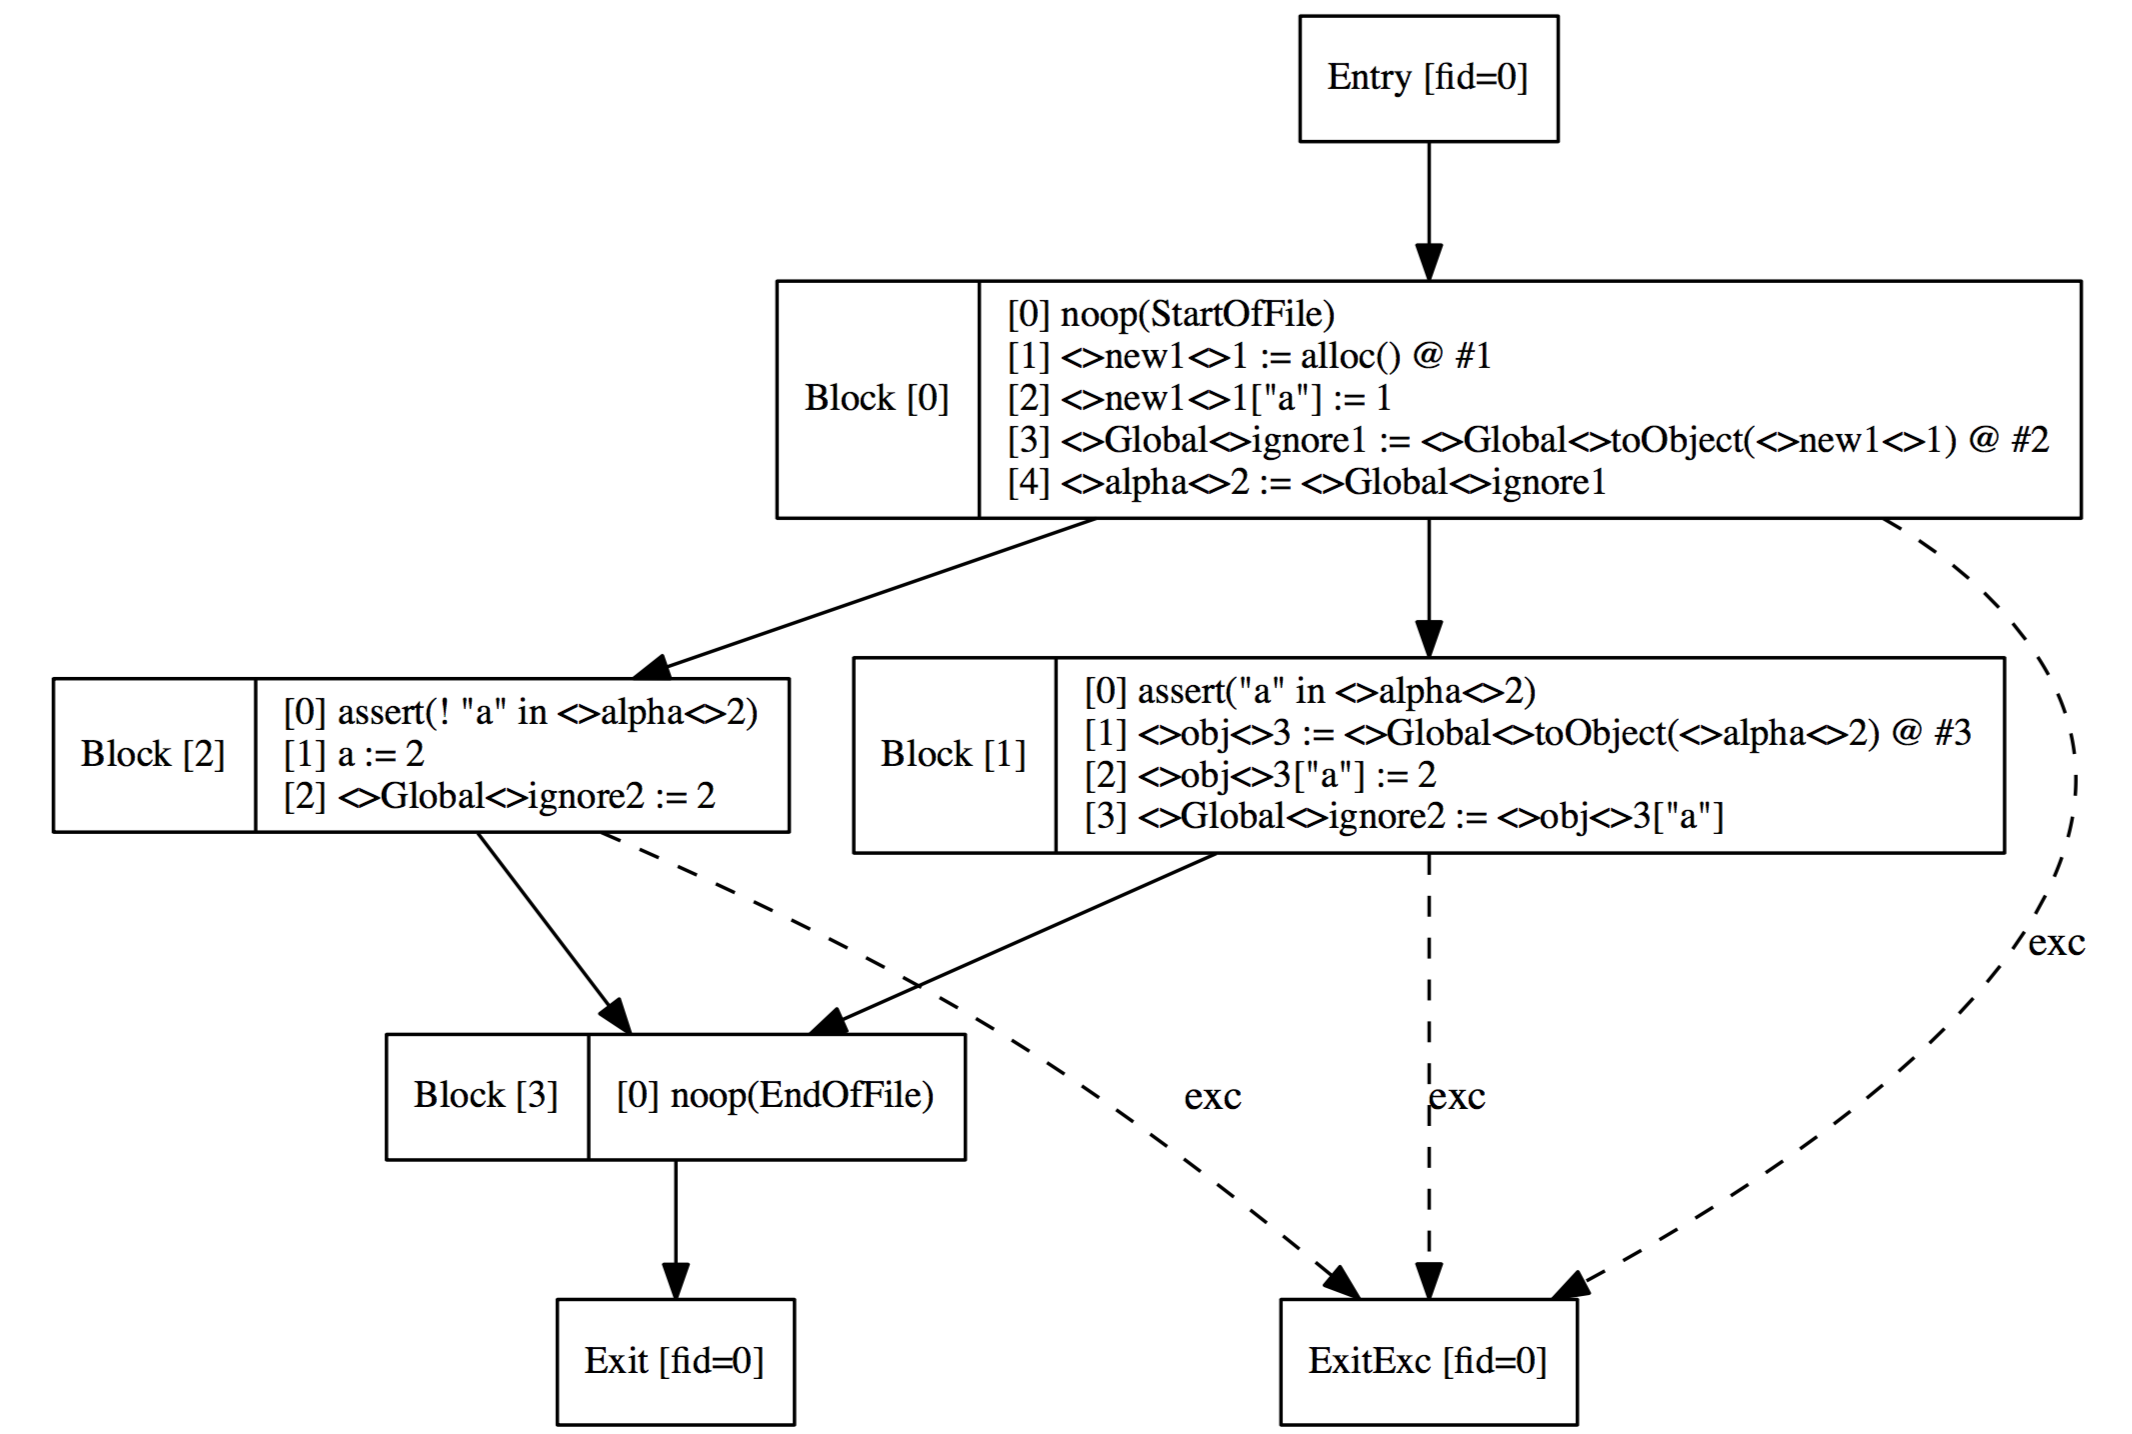
\includegraphics[width=8.75cm]{cfg.png}
\end{figure}

\section{\safe analyzer debugging}
When the \verb!-analyzer:console! option is given to the \texttt{analyze} command,
\safe provides a REPL-style console debugger.
For example, the following command:
\begin{verbatim}
safe analyze -analyzer:console test.js
\end{verbatim}
shows the list of available commands for debugging and
the starting point of the analysis:
{\small
\begin{verbatim}
Command list:
- help           
- next       jump to the next iteration. (same as "")
- jump       Continue to analyze until the given
             iteration.
- print      Print out various information.
- result     Print out various information.
- run_insts  Run instruction by instruction.
- move       Change a current position.
- home       Reset the current position.
- run        Run until meet some break point.
- break      Add a break point.
- break-list Show the list of break points.
- break-rm   Remove a break point.
For more information, see 'help <command>'.

<function[0] top-level: Entry[-1], ()> @test.js:1:1
Iter[0] > 
\end{verbatim}
}

The current status is denoted as follows:
{\small
\begin{verbatim}
<function [{fid}] {fun-name}: {block-kind}[{bid}],
 {call-context}> @{filename}:{span}
Iter[{#iteration}] >
\end{verbatim}
}
\noindent
where \verb!fid! and \verb!fun-name! are the id and the name of the current function,
respectively, \verb!block-kind! and \verb!bid!
are the kind and the id of the current block, respectively,
\verb!call-context! is the call context of the current analysis,
\verb!filename! is the name of the file being analyzed,
\verb!span! is the location of the current analysis, and
\verb!#iteration! is the iteration number of the current analysis.

A block is one of the following kinds:
\begin{itemize}
\itemsep-.1em
\item Entry: the entry block of a function
\item Block: a normal block with instructions
\item Exit: the exit block of a function
\item ExitExc: a block denoting uncaught exceptions in a function
\item Call: a block denoting a function call
\item AfterCall: a block receiving a return value of a function call
\item AfterCatch: a block receiving uncaught exceptions after a function call
\item ModelBlock: a block denoting a modeled function
\end{itemize}

The \verb!help! command displays a list of available commands and
the \verb!help <command>! command displays the usage of the \verb!<command>!.
For example:
{\small
\begin{verbatim}
<function[0] top-level: Entry[-1], ()> @test.js:1:1
Iter[0] > help print
usage: print state(-all) ({keyword})
       print block
       print loc {LocName} ({keyword})
       print fid {functionID}
       print worklist
       print ipsucc
       print trace
       print cfg
\end{verbatim}
}
\noindent
shows the usage of the \verb!print! command.

\medskip
The \verb!next! command proceeds the analysis of the current block,
which is the default command.  For example:
{\small
\begin{verbatim}
<function[0] top-level: Entry[-1], ()> @test.js:1:1
Iter[0] >

<function[0] top-level: Block[0], ()> @test.js:1:1-7:18
Iter[1] >
\end{verbatim}
}

\medskip
The \verb!jump {#iteration}! command proceeds the analysis until the given
number of iterations.  For example:
{\small
\begin{verbatim}
<function[0] top-level: Entry[-1], ()> @test.js:1:1
Iter[0] > jump 10

<function[0] top-level: Block[4], ()> @test.js:7:5-21:1
Iter[10] >
\end{verbatim}
}

\medskip
The \verb!print! command displays the status just before
analyzing the current block.  We describe it in Section~\ref{s:3:2:1:refman}.

\medskip
The \verb!result! command displays the status after analyzing
the current block:
\begin{itemize}
\item \verb!result (exc-)state(-all) ({keyword})!

It displays the state in the same way as the \verb!print! command does,
and it can additionally show the exception state generated after the analysis.
\item \verb!result (exc-)loc {LocName}!

It finds and displays the location in the same way as the \verb!print! command does,
and it can additionally find and display the location from
the exception state generated after the analysis.
\end{itemize}

\medskip
The \verb!run_insts! command shows the list of instructions in the current block,
and it enables to analyze each instruction.  It opens a sub-console, which provides 3 kinds
of commands:
\begin{itemize}
\itemsep-.1em
\item \verb!s! shows the state
\item \verb!q! quits the analysis
\item \verb!n! analyzes the next instruction; the default command
\end{itemize}
For example:
{\small
\begin{verbatim}
<function[0] top-level: Block[4], ()> @test.js:8:5-26:1
Iter[10] > run_insts 
Block[4] -> Exit, ExitExc
  [0] shift := <>Global<>ignore6
  [1] __result1 := shift !== "x"
  [2] __expect1 := false
  [3] <>obj<>10 := <>Global<>toObject(obj) @ #13
  [4] __result2 := <>obj<>10["length"] !== 1
  [5] __expect2 := false
  [6] <>obj<>11 := <>Global<>toObject(obj) @ #14
  [7] __result3 := <>obj<>11[0] !== "y"
  [8] __expect3 := false
  [9] <>obj<>12 := <>Global<>toObject(obj) @ #15
  [10] __result4 := <>obj<>12[1] !== undefined
  [11] __expect4 := false
  [12] noop(EndOfFile)

inst: [0] shift := <>Global<>ignore6
('s': state / 'q': stop / 'n','': next)
>

inst: [1] __result1 := shift !== "x"
('s': state / 'q': stop / 'n','': next)
> 
\end{verbatim}
}

\medskip
The \verb!move {fid}:{{bid}|entry|exit|exitExc}! command
moves the current block to the given block denoted by the id of a function,
the id of a block, and the kind of the block.  For example:
{\small
\begin{verbatim}
<function[0] top-level: ExitExc[-3], ()> @test.js:26:1
Iter[12] > move 0:exit
* current control point changed.

<function[0] top-level: Exit[-2], ()> @test.js:26:1
Iter[12] >
\end{verbatim}
}

\medskip
The \verb!home! command moves the current block back to the original
block to be analyzed.  For example:
{\small
\begin{verbatim}
<function[0] top-level: Exit[-2], ()> @test.js:26:1
Iter[12] > home
* reset the current control point.

<function[0] top-level: ExitExc[-3], ()> @test.js:26:1
Iter[12] >
\end{verbatim}
}

\medskip
The \verb!run! command proceeds the analysis until encountering a break
point.  A short-key for this command is Ctrl-d.  For example:
{\small
\begin{verbatim}
<function[0] top-level: Entry[-1], ()> @test.js:1:1
Iter[0] > break 0:exit

<function[0] top-level: Entry[-1], ()> @test.js:1:1
Iter[0] > run

<function[0] top-level: Exit[-2], ()> @test.js:26:1
Iter[11] >
\end{verbatim}
}

\medskip
The \verb!break! command sets up a break point at the given block.
For example:
{\small
\begin{verbatim}
<function[0] top-level: Entry[-1], ()> @test.js:1:1
Iter[0] > break 0:exit

<function[0] top-level: Entry[-1], ()> @test.js:1:1
Iter[0] > run

<function[0] top-level: Exit[-2], ()> @test.js:26:1
Iter[11] >
\end{verbatim}
}

\medskip
The \verb!break-list! command shows a list of blocks with
break points.  For example:
{\small
\begin{verbatim}
<function[0] top-level: Exit[-2], ()> @test.js:26:1
Iter[11] > break-list
* 2 break point(s).
  [0] function[0] Exit[-2]
  [1] function[0] Entry[-1]
\end{verbatim}
}

\medskip
The \verb!break-rm {break-order}! command
removes the break point of a given block
denoted by the order in the result of \verb!break-list!.
For example:
{\small
\begin{verbatim}
<function[0] top-level: Exit[-2], ()> @test.js:26:1
Iter[11] > break-list
* 2 break point(s).
  [0] function[0] Exit[-2]
  [1] function[0] Entry[-1]

<function[0] top-level: Exit[-2], ()> @test.js:26:1
Iter[11] > break-rm 0
* break-point[0] removed.
[0] function[0] Exit[-2]

<function[0] top-level: Exit[-2], ()> @test.js:26:1
Iter[11] > break-list
* 1 break point(s).
  [0] function[0] Entry[-1]
\end{verbatim}
}

\subsection{Analyzer debugging with printing}
\label{s:3:2:1:refman}
The \verb!print! command displays the status just before
analyzing the current block.

\medskip\noindent
\fbox{\texttt{print state(-all) (\{keyword\})}}\\[.2em]
The \verb!print state! command displays the current state,
and the \verb!print state-all! command
displays the current state including all system addresses.
When a keyword is given, it displays only the parts that include the keyword.
For example:
{\small
\begin{verbatim}
<function[0] top-level: Exit[-2], ()> @test.js:21:1
Iter[12] > print state result
           "__result1" -> [ttf] false
           "__result2" -> [ttf] false
           "__result3" -> [ttf] false
           Set(NaN, __result3, Function,
__EvalErrLoc, URIError, pop, JSON, Error, Number,
decodeURIComponent, __SyntaxErrProtoLoc, RangeError,
__RangeErrLoc, __ArrayConstLoc, __EvalErrProtoLoc,
Boolean, ReferenceError, __RefErrLoc, obj, __BOT,
encodeURIComponent, __TypeErrProtoLoc, Array,
EvalError, __expect1, encodeURI, eval, __expect3,
isFinite, __ErrProtoLoc, Object, __TOP, Math,
__TypeErrLoc, __URIErrProtoLoc, __result1,
parseFloat, __RangeErrProtoLoc, TypeError,
<>Global<>global, __ObjConstLoc, isNaN, __URIErrLoc,
Date, __NumTop, __expect2, decodeURI, RegExp,
__BoolTop, __UInt, parseInt, __result2, __StrTop,
Infinity, SyntaxError, __RefErrProtoLoc, __Global,
<>Global<>true, __SyntaxErrLoc, undefined, String)
\end{verbatim}
}

\medskip\noindent
\fbox{\texttt{print block}}\\[.2em]
The \verb!print block! command displays the information of
a given block.  For example:
{\small
\begin{verbatim}
<function[0] top-level: Block[0], ()> @test.js:1:1-7:18
Iter[1] > print block
Block[0] -> [1], ExitExc
  [0] noop(StartOfFile)
  [1] <>Global<>ignore1 := alloc() @ #1
  [2] obj := <>Global<>ignore1
  [3] <>obj<>1 := <>Global<>toObject(obj) @ #2
  [4] <>obj<>2 := <>Global<>toObject(Array) @ #3
  [5] <>obj<>3 :=
      <>Global<>toObject(<>obj<>2["prototype"]) @ #4
  [6] <>obj<>1["pop"] := <>obj<>3["pop"]
  [7] <>obj<>4 := <>Global<>toObject(obj) @ #5
  [8] <>obj<>4[4294967294] := "x"
  [9] <>obj<>5 := <>Global<>toObject(obj) @ #6
  [10] <>obj<>5["length"] := - 1
  [11] <>obj<>6 := <>Global<>toObject(obj) @ #7
  [12] <>arguments<>7 := allocArg(0) @ #8
  [13] <>fun<>8 :=
       <>Global<>toObject(<>obj<>6["pop"]) @ #9
\end{verbatim}
}

\medskip\noindent
\fbox{\texttt{print loc \{LocName\} (\{keyword\})}}\\[.2em]
The \verb!print loc {LocName}! command shows the object
bound at a given location in the current state.
When a keyword is given, it displays only the parts that include the keyword
in the object.  For example:
{\small
\begin{verbatim}
<function[0] top-level: ExitExc[-3], ()> @test.js:21:1
Iter[12] > print loc #1
#1 -> [[Class]] : "Object"
      [[Extensible]] : true
      [[Prototype]] : #Object.prototype
      "4294967294" -> [ttt] "x"
      "length" -> [ttt] -1
      "pop" -> [ttt] #Array.prototype.pop
      Set(pop, length, 4294967294)
\end{verbatim}
}

\medskip\noindent
\fbox{\texttt{print fid \{functionID\}}}\\[.2em]
It displays the name and the span information of
a given function id.  For example:
{\small
\begin{verbatim}
<function[0] top-level: ExitExc[-3], ()> @test.js:21:1
Iter[12] > print fid 0
* function name: top-level
* span info.   : test.js:1:1-21:1
\end{verbatim}
}

\medskip\noindent
\fbox{\texttt{print worklist}}\\[.2em]
It shows the work in the current worklist.  For example:
{\small
\begin{verbatim}
<function[42] []Array.prototype.pop: ExitExc[-3],
 (10)> @[]Array.prototype.pop:0:0
Iter[6] > print worklist
* Worklist set
(42:ExitExc[-3], (10)), (42:Exit[-2], (10)),
(0:AfterCall[2], ()), (0:ExitExc[-3], ())
\end{verbatim}
}

\medskip\noindent
\fbox{\texttt{print ipsucc}}\\[.2em]
It displays the information of the current inter-procedural successor.
For example:
{\small
\begin{verbatim}
<function[42] []Array.prototype.pop: ExitExc[-3],
 (10)> @[]Array.prototype.pop:0:0
Iter[6] > print ipsucc
* successor map
- src: FlowSensitiveCP(ExitExc[-3],(10))
- dst: FlowSensitiveCP(AfterCatch[3],()),
 mayOld: (10, 1, 8)
mustOld: (10, 1, 8)
\end{verbatim}
}

\medskip\noindent
\fbox{\texttt{print trace}}\\[.2em]
It shows the current call trace.  For example:
{\small
\begin{verbatim}
<function[42] []Array.prototype.pop: Entry[-1],
 (10)> @[]Array.prototype.pop:0:0
Iter[3] > print trace
* Call-Context Trace
Entry[-1] of function[42] []Array.prototype.pop with (10)
 1>  [0] call(<>fun<>8, <>obj<>6, <>arguments<>7) @ #10
test.js:7:11-20 @Call[1] of function[0] top-level with ()
\end{verbatim}
}

\medskip\noindent
\fbox{\texttt{print cfg}}\\[.2em]
It prints the current CFG to files \verb!cfg.gv! and \verb!cfg.pdf!.

\medskip\noindent
\fbox{\texttt{print html}}\\[.2em]
It prints the current CFG and its state to the \verb!cfg.html! file.
We describe this facility in the next section.

\subsection{Analyzer debugging with browsing}
\label{s:3:2:2:refman}
The \verb!print html! command writes the current status into an HTML file
so that a user can investigate the analysis status from a browser.
Consider the following snapshot:
\begin{figure}[H]
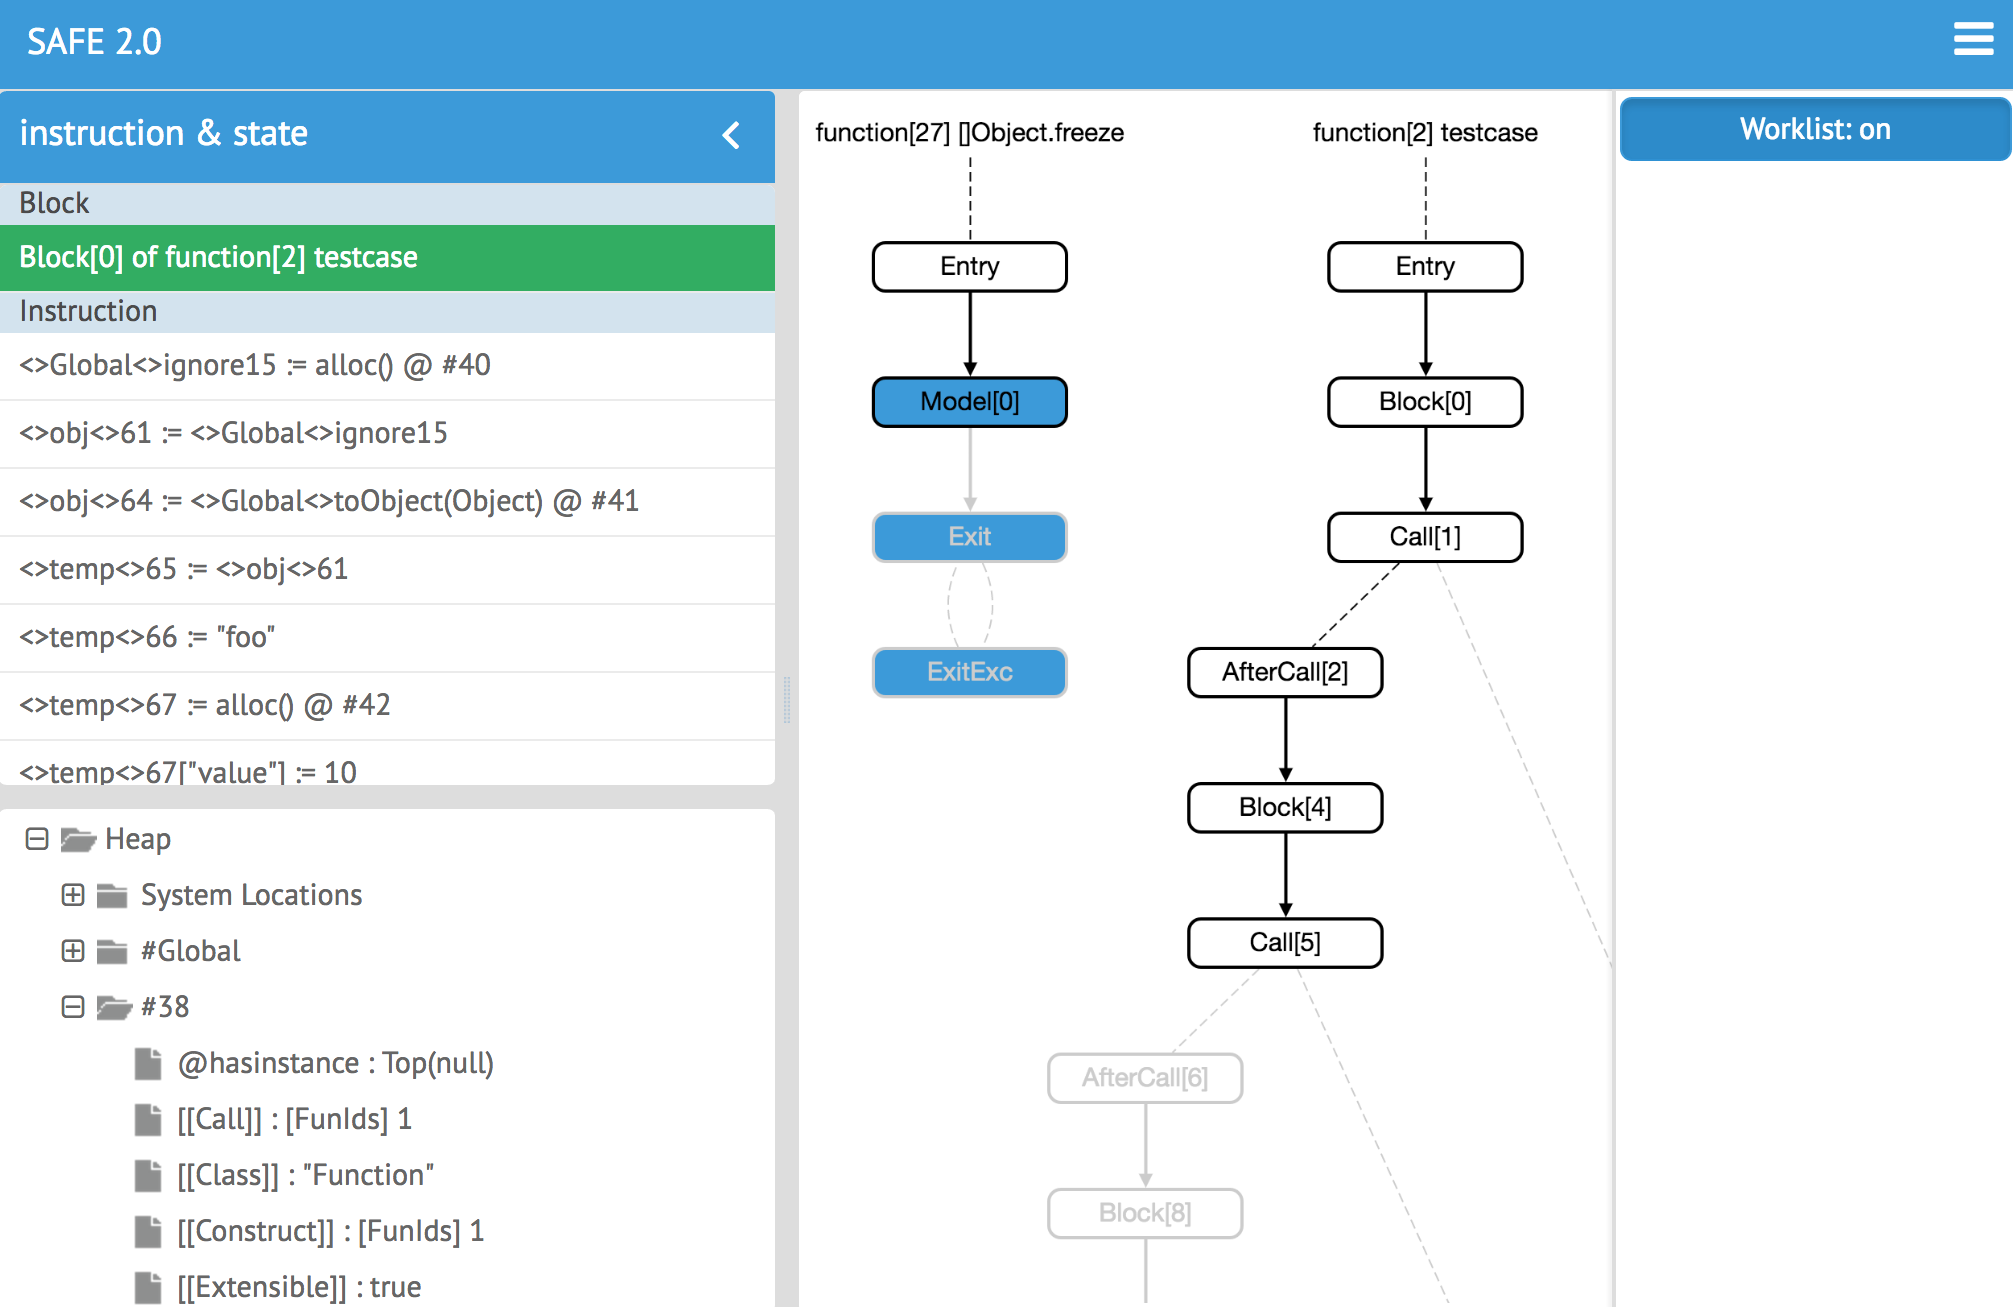
\includegraphics[width=8.75cm]{htmldebugger.png}
\end{figure}
\noindent
which shows the current CFG in the middle.
Nodes in black lines denote the blocks that are analyzed,
those in gray lines denote the blocks not yet being analyzed, and
colored nodes denote the blocks that are currently in the worklist of the analyzer.
One can toggle whether to show the nodes in the worklist by the menu button on the top right.
When a user selects a block from the CFG, the list of the instructions in the block
and the state just before analyzing the block are displayed on the left.


%--------------------------------------------------------------------
% Appendix
%--------------------------------------------------------------------
\appendix
% thicker vertical line
\newcolumntype{?}{!{\vrule width 1pt}}

% Styles
\definecolor{dkgreen}{rgb}{0,0.6,0}
\definecolor{gray}{rgb}{0.5,0.5,0.5}
\definecolor{mauve}{rgb}{0.58,0,0.82}
\lstdefinelanguage{JavaScript}{
  keywords={async, await, break, case, catch, class, const, continue, debugger,
    default, delete, do, else, enum, export, extends, false, finally, for,
    function, if, import, in, instanceof, new, null, return, super, switch, this,
    throw, true, try, typeof, var, void, while, with, yield},
  keywordstyle=\color{blue}\bfseries,
  ndkeywordstyle=\color{darkgray}\bfseries,
  identifierstyle=\color{black},
  sensitive=false,
  comment=[l]{//},
  morecomment=[s]{/*}{*/},
  commentstyle=\color{dkgreen}\ttfamily,
  stringstyle=\color{purple}\ttfamily,
  morestring=[b]',
  morestring=[b]"
}
\lstdefinestyle{myJSstyle}{
  language=JavaScript,
  numbers=left,
  stepnumber=1,
  extendedchars=true,
  basicstyle=\footnotesize\ttfamily,
  showstringspaces=false,
  showspaces=false,
  tabsize=2,
  breaklines=true,
  showtabs=false,
  captionpos=b
}

% Basic
\DeclareMathAlphabet{\mathpzc}{T1}{pzc}{m}{it}
\newcommand{\powerset}[1]{\mathcal{P}(#1)}
\newcommand{\imbox}[1]{\mbox{\small \textit{#1}}}
\newcommand{\name}[1]{\textsf{#1}}
\newcommand{\inred}[1]{{\color{red}{#1}}}
\newcommand{\todo}{\inred{TODO}}
\newcommand{\abs}[1]{{#1}^{\#}}
\newcommand{\finmap}{{\xrightarrow[]{\text{fin}}}}
\newcommand{\mapstos}{\;\dot{\mapsto}\;}
\newcommand{\Dom}{\name{Dom}}

% Tool
\newcommand{\tool}{\text{SAFE}_\name{DS}}

% Keywords
\newcommand{\jscode}[1]{\text{\lstinline[style=myJSstyle,numbers=none]!#1!}}
\newcommand{\code}[1]{\texttt{#1}}
\newcommand{\kwif}{\code{if}}
\newcommand{\kwelse}{\code{else}}
\newcommand{\kwret}{\code{ret}}
\newcommand{\kwobj}{\code{\{\}}}
\newcommand{\kwtrue}{\code{true}}
\newcommand{\kwfalse}{\code{false}}

% Notations
\newcommand{\prog}{P}
\newcommand{\labset}{\mathcal{L}}
\newcommand{\lab}{\mathpzc{l}}
\newcommand{\labdot}[1]{{{\bullet_{\lab_{#1}}}}}
\newcommand{\ilab}{\lab_\iota}
\newcommand{\labnext}{\name{next}}
\newcommand{\op}{\name{op}}
\newcommand{\ops}{\dot{\name{op}}}
\newcommand{\inst}{i}
\newcommand{\expr}{e}
\newcommand{\refer}{r}

% Numbers
\newcommand{\numset}{\mathbb{N}}

% States
\newcommand{\stset}{\mathbb{S}}
\newcommand{\st}{\sigma}
\newcommand{\istset}{\stset_\iota}
\newcommand{\ist}{\st_\iota}

% Memories
\newcommand{\memset}{\mathcal{M}}
\newcommand{\absmemset}{\abs{\memset}}
\newcommand{\mem}{M}
\newcommand{\absmem}{\abs{\mem}}

% Contexts
\newcommand{\ctxtset}{\mathbb{C}}
\newcommand{\absctxtset}{\abs{\ctxtset}}
\newcommand{\ctxt}{c}
\newcommand{\absctxt}{\abs{\ctxt}}
\newcommand{\eabsctxt}{\absctxt_\name{env}}

% Transition Relations
\newcommand{\trans}{\leadsto}
\newcommand{\rutrans}{%
            \mathrel{\raisebox{.1em}{%
            \rotatebox[origin=c]{30}{$\trans$}}}}
\newcommand{\rdtrans}{%
            \mathrel{\raisebox{.1em}{%
            \rotatebox[origin=c]{-30}{$\trans$}}}}


% Complete Lattice
\newcommand{\join}{\sqcup}
\newcommand{\meet}{\sqcap}
\newcommand{\bigjoin}{\bigsqcup}
\newcommand{\bigmeet}{\bigsqcap}
\newcommand{\order}{\sqsubseteq}

% Concrete Domains
\newcommand{\dom}{\mathbb{D}}
\newcommand{\elem}{d}
\newcommand{\ielem}{\elem_\iota}

% Abstract Domains
\newcommand{\absdom}{\abs{\dom}}
\newcommand{\abselem}{\abs{\elem}}
\newcommand{\iabselem}{\abs{\elem}_\iota}

% Concrete Semantics
\newcommand{\sem}[1]{[\![{#1}]\!]}
\newcommand{\transfer}{F}
\newcommand{\step}{\name{step}}

% Abstract Semantics
\newcommand{\abssem}[1]{\abs{\sem{#1}}}
\newcommand{\abstransfer}{\abs{\transfer}}
\newcommand{\absstep}{\abs{\step}}

% Abstract Sensitivity
\newcommand{\viewmap}{\delta}
\newcommand{\sabsdom}{\absdom_\viewmap}
\newcommand{\sabselem}{{\abselem_\viewmap}}
\newcommand{\viewset}{\Pi}
\newcommand{\view}{\pi}
\newcommand{\sabsstep}{\absstep_\viewmap}
\newcommand{\viewtrans}[2]{\abssem{#1 \rightarrow #2}}

% Flow Sensitivity
\newcommand{\fs}{\name{FS}}
\newcommand{\fsviewmap}{\viewmap^\fs}

% Locations
\newcommand{\locset}{\mathbb{L}}
\newcommand{\loc}{l}
\newcommand{\abslocset}{\abs\locset}
\newcommand{\absloc}{\abs\loc}

% Variables
\newcommand{\varset}{\mathbb{X}}
\newcommand{\varx}{\code{x}}

% Values
\newcommand{\valset}{\mathbb{V}}
\newcommand{\val}{v}
\newcommand{\pvalset}{\valset_\name{p}}
\newcommand{\pval}{\val_\name{p}}
\newcommand{\fvalset}{\mathbb{F}}
\newcommand{\fval}[2]{\lambda #1. #2}
\newcommand{\strset}{\valset_\name{str}}
\newcommand{\str}{\val_\name{str}}
\newcommand{\absvalset}{\abs{\valset}}
\newcommand{\absval}{\abs{\val}}

\newcommand{\valgamma}{\gamma_\val}

% Addresses
\newcommand{\addrset}{\mathbb{A}}
\newcommand{\eaddrset}{\addrset_\name{env}}
\newcommand{\oaddrset}{\addrset_\name{obj}}
\newcommand{\addr}{a}
\newcommand{\tladdr}{\addr_{\name{top}}}
\newcommand{\absaddrset}{\abs{\addrset}}
\newcommand{\absaddr}{\abs{\addr}}
\newcommand{\eabsaddr}{\absaddr_\name{env}}
\newcommand{\rabsaddr}{\absaddr_\name{ret}}
\newcommand{\oabsaddr}{\absaddr_\name{obj}}

% Abstract Counting
\newcommand{\abscount}{\abs{n}}
\newcommand{\inc}{\name{inc}}
\newcommand{\abscountset}{\abs{\mathbb{N}}}
\newcommand{\abszero}{\abs{0}}
\newcommand{\absone}{\abs{1}}
\newcommand{\absmany}{\abs{\geq\!\!2}}

% Sealed Symbolic Interpretation
\newcommand{\symb}{\omega}
\newcommand{\symbset}{\Omega}
\newcommand{\symbolic}[1]{{#1}_\symb}
\newcommand{\symbstset}{\symbolic{\stset}}
\newcommand{\symbst}{\symbolic{\st}}
\newcommand{\nsymbst}[1]{\st_{\symb,#1}}
\newcommand{\symbmemset}{\symbolic{\memset}}
\newcommand{\symbtrans}{\symbolic{\trans}}
\newcommand{\excst}{\bot}
\newcommand{\symbevt}{\symb_\jscode{evt}}
\newcommand{\symbint}{\symb_\jscode{int}}

% Combined Analysis
\newcommand{\comb}[1]{\widetilde{#1}}
\newcommand{\combdom}{\comb{\dom}}
\newcommand{\combelem}{\comb{\elem}}
\newcommand{\combgamma}{\comb{\gamma}}
\newcommand{\combstep}{\comb{\step}}
\newcommand{\combtransfer}{\comb{\transfer}}
\newcommand{\sgamma}{\gamma_\viewmap}
\newcommand{\converter}{\tau}
\newcommand{\saconverter}{\abs{\converter}}
\newcommand{\asconverter}{\symbolic{\converter}}
\newcommand{\combviewtrans}[2]{\sem{\comb{#1 \rightarrow #2}}}

\newcommand{\symbdom}{\symbolic{\dom}}
\newcommand{\symbelem}{\symbolic{\elem}}
\newcommand{\symbgamma}{\symbolic{\gamma}}
\newcommand{\symbstep}{\symbolic{\step}}

% Legacy
\newcommand{\scombstep}{\comb{\step}_\viewmap}
\newcommand{\scombgamma}{\combgamma_\viewmap}
\newcommand{\scombelem}{\comb{\elem}_\viewmap}

% Triage
\newcommand{\triage}{\name{triage}}
\newcommand{\atriage}{\triage_\aelem}

% Rules
\newcommand{\referrule}[3]{#1 \vdash_\refer #2 \Rightarrow  #3}
\newcommand{\exprrule}[3]{#1 \vdash_\expr #2 \Rightarrow #3}

% Abstract Semantics
\newcommand{\referabssem}[1]{\abssem{#1}_\refer}
\newcommand{\exprabssem}[1]{\abssem{#1}_\expr}

% Identity function
\newcommand{\identity}{\name{id}}

% Checker
\newcommand{\checker}{\name{checker}}

% Concerto
\newcommand{\concerto}{\textsc{Concerto}}

% Table 1
\newcommand{\myhead}[3]{
  \multicolumn{1}{c|}{\textbf{#1}} &
  \multicolumn{1}{c|@{~}}{\textbf{#2}} &
  \multicolumn{4}{@{~}c@{~}?}{\textbf{#3}} &
  \multicolumn{1}{c|}{\textbf{#1}} &
  \multicolumn{1}{c|@{~}}{\textbf{#2}} &
  \multicolumn{4}{@{~}c@{~}?}{\textbf{#3}} &
  \multicolumn{1}{c|}{\textbf{#1}} &
  \multicolumn{1}{c|@{~}}{\textbf{#2}} &
  \multicolumn{4}{@{~}c@{~}}{\textbf{#3}}\\\hline
}
\newcommand{\mydata}[6]{
  \multirow{#1}{*}{\jscode{#2}} &
  \jscode{#3} &
  \text{#4} &
  \text{/} &
  \text{#5} &
  \text{(#6\%)}
}
\newcommand{\mysucccolor}{yellow}
\newcommand{\mysucc}[6]{
  \multirow{#1}{*}{\jscode{#2}} &
  \multicolumn{1}{>{\columncolor{\mysucccolor}}l|@{~}}    {\jscode{#3}} &
  {\text{#4}} &
  {\text{/}} &
  {\text{#5}} &
  {\text{(#6\%)}}
}
\newcommand{\mymult}[6]{
  \jscode{#2} &
  \multirow{#1}{*}{\jscode{#3}} &
  \multirow{#1}{*}{\text{#4}} &
  \multirow{#1}{*}{\text{/}} &
  \multirow{#1}{*}{\text{#5}} &
  \multirow{#1}{*}{\text{(#6\%)}}
}
\newcommand{\myname}[2]{\multirow{#1}{*}{\jscode{#2}}&&&&&}
\newcommand{\mynewline}[6]{
  \\
  \cline{#1-#2}
  \cline{#3-#4}
  \cline{#5-#6}
}
\newcommand{\mylinef}  {\\\hhline{~|-----}}
\newcommand{\mylineff} {\\\hhline{~|-----~|-----}}
\newcommand{\mylinetf} {\\\hhline{------~|-----}}
\newcommand{\mylinefff}{\\\hhline{~|-----~|-----~|-----}}
\newcommand{\mylinefft}{\\\hhline{~|-----~|-----------}}
\newcommand{\mylineftf}{\\\hhline{~|-----------~|-----}}
\newcommand{\mylineftt}{\\\hhline{~|-----------------}}
\newcommand{\mylinetff}{\\\hhline{------~|-----~|-----}}
\newcommand{\mylinetft}{\\\hhline{------~|-----------}}
\newcommand{\mylinettf}{\\\hhline{------------~|-----}}
\newcommand{\mylinettt}{\\\hhline{------------------}}

% Instantiation Map
\newcommand{\imap}{m}
\newcommand{\imapset}{\mathbb{M}}
\newcommand{\absimap}{\abs{\imap}}
\newcommand{\absimapset}{\abs{\imapset}}
\newcommand{\instant}[2]{#1\!\!\mid\!\!_{#2}}
\newcommand{\imapgamma}{\gamma_\imap}

% Analysis Element
\newcommand{\aelem}{\epsilon}
\newcommand{\aelemset}{\mathbb{E}}
\newcommand{\aelemgamma}{\gamma_{\aelem}}

% Difference Set
\newcommand{\diffset}{\Delta}

\chapter{Appendix}

This appendix provides the definitions of
AST, IR, and translation rules from AST to IR in \safe.

\section{AST}
This section describes each construct of the JavaScript language
in both the BNF notation and its corresponding implementation.
The implementation of AST nodes is available at:
\begin{verbatim}
$SAFE_HOME/src/main/scala/kr/ac/kaist/safe/nodes/
           ast/
\end{verbatim}
\small
\[
\begin{array}{llll}
\pgm & ::=  & \fd^*\ \vd^*\ \stmt^* \\
&& \mtt{Program(body:~TopLevel)}\\
    &&\mtt{TopLevel(fds:~List[FunDecl], vds:~List[VarDecl],}\\
&&\mtt{\phantom{TopLevel(}stmts:~List[SourceElements])}\\\\

\fd &::=& {\tt function} \ f \verb+(+(x\verb+,+)^*\verb+)+ \ \verb+{+\fd^*\ \vd^*\ \stmt^*\verb+}+\\
&& \mtt{FunDecl(ftn:~Functional, strict:~Boolean)}\\
&& \mtt{Functional(fds:~List[FunDecl],}\\
&&\mtt{\phantom{Functional(}vds:~List[VarDecl],}\\
&&\mtt{\phantom{Functional(}stmts:~SourceElements, name:~Id,}\\
&&\mtt{\phantom{Functional(}params:~List[Id], body:~String)}\\\\

\vd &::=& x \ ({\tt =} \ \expr)^? \\
&& \mtt{VarDecl(name:~Id, expr:~Option[Expr],}\\
&& \mtt{\phantom{VarDecl(}strict:~Boolean)}\\\\

\stmt &::=& \verb+{+\stmt^*\verb+}+ \\
&& \mtt{ABlock(stmts:~List[Stmt], internal:~Boolean)}\\
& \mid & {\tt var} \ \vd(\verb+,+ \vd)^* \verb+;+ \\
&& \mtt{VarStmt(vds:~List[VarDecl])}\\
& \mid & \verb+;+ \\
&& \mtt{EmptyStmt()}\\
& \mid & \expr \verb+;+ \\
&& \mtt{ExprStmt(expr:~Expr, internal:~Boolean)}\\
& \mid & {\tt if} \ \verb+(+\expr\verb+)+ \ \stmt \ ({\tt else} \ \stmt)^?\\
&& \mtt{If(cond:~Expr, trueBranch:~Stmt,}\\
&&\mtt{\phantom{If(}falseBranch:~Option[Stmt])}\\
\end{array}
\]

\[
\begin{array}{llll}
& \mid &  {\tt switch} \ \verb+(+\expr\verb+)+ \ \verb+{+\cc^* \ ({\tt default} \verb+:+ \stmt^{*})^? \ \cc^* \verb+}+\\
&& \mtt{Switch(cond:~Expr, frontCases:~List[Case],}\\
&&\mtt{\phantom{Switch(}defopt:~Option[List[Stmt]],}\\
&&\mtt{\phantom{Switch(}backCases:~List[Case])}\\
& \mid & {\tt do} \ \stmt \ {\tt while} \ \verb+(+\expr\verb+)+ \verb+;+ \\
&& \mtt{DoWhile(body:~Stmt, cond:~Expr)}\\
  &\mid& {\tt while} \ \verb+(+\expr\verb+)+ \ \stmt \\
&& \mtt{While(cond:~Expr, body:~Stmt)}\\
  &\mid& {\tt for} \ \verb+(+\expr^?\verb+;+ \expr^?\verb+;+ \expr^? \verb+)+ \ \stmt\\
&& \mtt{For(init:~Option[Expr], cond:~Option[Expr],}\\
&&\mtt{\phantom{For(}action:~Option[Expr], body:~Stmt)}\\
  &\mid& {\tt for} \ \verb+(+ \lhs \ {\tt in} \ \expr \verb+)+ \ \stmt \\
&&\mtt{ForIn(lhs:~LHS, expr:~Expr, body:~Stmt)}\\
  &\mid& {\tt for} \ \verb+(+{\tt var} \ \vd(\verb+,+ \vd)^*\verb+;+ \expr^?\verb+;+ \expr^?\verb+)+ \ \stmt\\
&& \mtt{ForVar(vars:~List[VarDecl], cond:~Option[Expr],}\\
&&\mtt{\phantom{ForVar(}action:~Option[Expr], body:~Stmt)}\\
&\mid& {\tt for} \ \verb+(+{\tt var} \ \vd \ {\tt in} \ \expr \verb+)+ \ \stmt \\
&& \mtt{ForVarIn(vd:~VarDecl, expr:~Expr, body:~Stmt)}\\
& \mid & {\tt continue} \  \myid^{?} \verb+;+ \\
&& \mtt{Continue(target:~Option[Label])}\\
& \mid & {\tt break} \  \myid^{?} \verb+;+ \\
&& \mtt{Break(target:~Option[Label])}\\
& \mid & {\tt return} \ \expr^? \verb+;+ \\
&& \mtt{Return(expr:~Option[Expr])}\\
& \mid & {\tt with} \ \verb+(+\expr\verb+)+ \ \stmt \\
&& \mtt{With(expr:~Expr, stmt:~Stmt)}\\
& \mid & l \; \verb+:+ \; \stmt \\
&& \mtt{LabelStmt(label:~Label, stmt:~Stmt)}\\
& \mid & {\tt throw} \ \expr \verb+;+ \\
&& \mtt{Throw(expr:~Expr)}\\

& \mid &
{\tt try} \verb+{+\stmt^*\verb+}+ ({\tt catch} \verb+(+\myid\verb+)+ \verb+{+\stmt^*\verb+}+)^? ({\tt finally} \verb+{+\stmt^*\verb+}+)^?\\
&& \mtt{Try(body:~List[Stmt], catchBlock:~Option[Catch],}\\
&& \mtt{\phantom{Try(}fin:~Option[List[Stmt]])}\\
&& \mtt{Catch(id:~Id, body:~List[Stmt])}\\
& \mid & {\tt debugger} \verb+;+ \\
&& \mtt{Debugger()}\\\\

\cc &::=& {\tt case} \ \expr \; \verb+:+ \; \stmt^{*} \\
&& \mtt{Case(cond:~Expr, body:~List[Stmt])}\\\\

\expr &::=& \expr\verb+,+ \ \expr \\
&& \mtt{ExprList(exprs:~List[Expr])}\\
  &\mid& \expr \ \verb+?+ \ \expr \ \verb+:+ \ \expr \\
&& \mtt{Cond(cond:~Expr, trueBranch:~Expr,}\\
&& \mtt{\phantom{Cond(}falseBranch:~Expr)}\\
  &\mid& \expr \ \inop \ \expr \\
&& \mtt{InfixOpApp(left:~Expr, op:~Op, right:~Expr)}\\
  &\mid& \preop \ \expr \\
&& \mtt{PrefixOpApp(op:~Op, right:~Expr)}\\
  &\mid& \lhs \ \postop \\
&& \mtt{UnaryAssignOpApp(lhs:~LHS, op:~Op)}\\
  &\mid& \lhs \ \aop \ \expr \\
&& \mtt{AssignOpApp(lhs:~LHS, op:~Op, right:~Expr)}\\
  &\mid& \lhs \\
&& \mtt{LHS()}\\\\
\end{array}
\]

\[
\begin{array}{llll}
\lhs &::=& \lit \\
&& \mtt{Literal()}\\
 &\mid& \myid \\
&& \mtt{VarRef(id:~Id)}\\
 &\mid& \verb+[+ (\expr^?\verb+,+)^* \ \verb+]+ \\
&& \mtt{ArrayExpr(elements:~List[Option[Expr]])}\\
 &\mid& \verb+{+ (\member\verb+,+)^* \verb+}+ \\
&& \mtt{ObjectExpr(members:~List[Member]}\\
 &\mid& \verb+(+ \expr \verb+)+ \\
&& \mtt{Parenthesized(expr:~Expr)}\\
 & \mid & {\tt function} \ \myid^?  \verb+(+(\myid\verb+,+)^*\verb+)+ \ \verb+{+\fd^*\ \vd^*\ \stmt^*\verb+}+ \\
&&\mtt{FunExpr(ftn:~Functional)}\\
 &\mid& \lhs \verb+[+ \expr \verb+]+ \\
&& \mtt{Bracket(obj:~LHS, index:~Expr)}\\
 &\mid& \lhs \verb+.+ \myid \\
&& \mtt{Dot(obj:~LHS, member:~Id)}\\
 &\mid& {\tt new} \ \lhs \\
&& \mtt{New(lhs:~LHS)}\\
 &\mid& \lhs \verb+(+ (\expr\verb+,+)^* \verb+)+ \\
&& \mtt{FunApp(fun:~LHS, args:~List[Expr])} \\ \\
\lit &::=& {\tt this} \\
&& \mtt{This()}\\
 &\mid& {\tt null} \\
&& \mtt{Null()}\\
 &\mid& {\tt true} \\
&& \mtt{Bool(bool:~Boolean)}\\
 &\mid& {\tt false} \\
&& \mtt{Bool(bool:~Boolean)}\\
 &\mid& \num \\
&& \mtt{DoubleLiteral(text:~String, num:~Double)}\\
&&\mtt{IntLiteral(intVal:~BigInteger, radix:~Integer)}\\
 &\mid& \str \\
&& \mtt{StringLiteral(quote:~String, escaped:~String)}\\
 &\mid& \reg \\
&& \mtt{RegularExpression(body:~String, flag:~String)}\\ \\

\member &::=& \prop \ \verb+:+ \ \expr \\
&& \mtt{Field(prop:~Property, expr:~Expr)}\\
 &\mid& {\tt get}\ \prop \verb+() {+ \fd^*\ \vd^*\ \stmt^* \verb+}+ \\
&& \mtt{GetProp(prop:~Property, ftn:~Functional)}\\
 &\mid& {\tt set}\ \prop \verb+(+ \myid \verb+) {+ \fd^*\ \vd^*\ \stmt^* \verb+}+\\
&& \mtt{SetProp(prop:~Property, ftn:~Functional)}\\ \\

\prop &::= & \myid \\
&& \mtt{PropId(id:~Id)}\\
 &\mid& \str \\
&& \mtt{PropStr(str:~String)}\\
 &\mid& \num \\
&& \mtt{PropNum(num:~NumberLiteral)}\\
\end{array}
\]

\[
\begin{array}{l@{\;}l@{\;}l@{\;}l@{\;}l@{\;}l@{\;}l@{\;}l@{\;}l@{\;}l@{\;}l@{\;}l@{\;}l@{\;}l@{\;}l@{\;}l@{\;}l@{\;}l@{\;}l@{\;}l@{\;}l@{\;}l@{\;}l@{\;}l@{\;}l@{\;}l@{\;}l@{\;}l@{\;}l@{\;}l@{\;}l@{\;}l@{\;}l@{\;}l@{\;}l@{\;}l@{\;}l@{\;}l@{\;}l@{\;}l@{\;}l@{\;}l@{\;}l@{\;}l@{\;}l@{\;}l@{\;}l}
\aop &::=&
\verb+=+ & \mid &
\verb+*=+ & \mid &
\verb+/=+ & \mid &
\verb+%=+ & \mid &
\verb!+=! & \mid &
\verb+-=+ & \mid &
\verb+[[=+ & \mid &
\verb+>>=+ & \mid &
\verb+>>>=+ & \mid &
\verb+&=+ & \mid &
\verb+^=+ & \mid &
\verb+|=+
\\

\inop &::=& \verb+&&+ & \mid & \verb+||+ & \mid & \verb+|+ & \mid & \verb+&+ & \mid & \verb+^+ & \mid & \verb+[[+ & \mid & \verb+>>+ & \mid & \verb+>>>+ 
 & \mid & \verb!+! & \mid & \verb+-+ & \mid & \verb+*+ & \mid & \verb+/+ \\
 & \mid & \verb+%+
 &\mid& \verb+==+ & \mid & \verb+!=+ & \mid & \verb+===+ & \mid & \verb+!==+ & \mid & \verb+[+ & \mid & \verb+>+ & \mid & \verb+[=+
 & \mid & \verb+>=+ \\
 & \mid &
\lefteqn{
 {\tt instanceof} \ \mid \ {\tt in} }\\

\preop &::=& \verb!++! & \mid & \verb+--+ & \mid & \verb+~+ & \mid & \verb+!+ & \mid & \verb!+! & \mid & \verb+-+ & \mid &
\lefteqn{
 {\tt delete} \ \mid \ {\tt void} \ \mid \ {\tt typeof} }\\

\postop &::=& \verb!++! & \mid & \verb+--+\\[1em]

\end{array}
\]

Note that after the \verb!Hoister! transformation of the \verb!astRewriter! phase,
ASTs should have the following invariants:
\begin{itemize}
\item The {\tt expr} field of {\tt VarDecl} should be {\tt None}.
\item {\tt VarStmt}, {\tt ForVar}, and {\tt ForVarIn} should be removed.
\item {\tt StmtUnit} is an internally generated statement unit.
\end{itemize}

\section{IR}
This section describes each construct of the \safe IR
in both the BNF notation and its corresponding implementation.
The implementation of IR nodes is available at:
\begin{verbatim}
$SAFE_HOME/src/main/scala/kr/ac/kaist/safe/nodes/ir/
\end{verbatim}
\small
\[
\begin{array}{llll}
\ir\pgm & ::= & \ir\stmt^* \\
&& \mtt{IRRoot(val fds:~List[IRFunDecl],}\\
&&\mtt{\phantom{IRRoot(}val vds:~List[IRVarStmt],}\\
&&\mtt{\phantom{IRRoot(}val irs:~List[IRStmt])}\\\\

\ir\stmt & ::= & \irid \ \verb+=+ \ \ir\expr \\
&& \mtt{IRExprStmt(val lhs:~IRId, val right:~IRExpr,}\\
&&\mtt{\phantom{IRExprStmt(}val ref:~Boolean)}\\
&\mid& \irid \ \verb+=+ \ {\sf delete}\ \irid\\
&& \mtt{IRDelete(val lhs:~IRId, val id:~IRId)}\\
&\mid& \irid \ \verb+=+ \ {\sf delete}\ \irid\verb+[+\irid\verb+]+\\
&& \mtt{IRDeleteProp(val lhs:~IRId, val obj:~IRId,}\\
&&\mtt{\phantom{IRDeleteProp(}val index:~IRExpr)}\\
&\mid& \irid\verb+[+\irid\verb+] =+ \ \irexpr \\
&& \mtt{IRStore(val obj:~IRId, val index:~IRExpr,}\\
&&\mtt{\phantom{IRStore(}val rhs:~IRExpr)}\\
 &\mid& \irid \ \verb+=+ \ \verb+{+ (\ir\member\verb+,+)^* \verb+}+\\
&& \mtt{IRObject(val lhs:~IRId, val members:~List[IRMember],}\\
&&\mtt{\phantom{IRObject(}val proto:~Option[IRId])}\\
 &\mid& \irid \ \verb+=+ \ \verb+[+ (\irexpr\verb+,+)^* \verb+]+ \\
&& \mtt{IRArray(val lhs:~IRId,}\\
&&\mtt{\phantom{IRArray(}val elements:~List[Option[IRExpr]])}\\
&&\mtt{IRArgs(val lhs:~IRId,}\\
&&\mtt{\phantom{IRArray(}val elements:~List[Option[IRExpr]])}\\
 &\mid& \irid \ \verb+=+ \ \irid\verb+(+\irid\verb+,+\irid\verb+)+\\
&& \mtt{IRCall(val lhs:~IRId, val fun:~IRId,}\\
&&\mtt{\phantom{IRCall(}val thisB:~IRId, val args:~IRId)}\\
 &\mid& \irid \ \verb+=+ \ \irid\verb+(+\irid(\verb+,+\irid)^?\verb+)+\\
&& \mtt{IRInternalCall(val lhs:~IRId, val fun:~IRId,}\\
&&\mtt{\phantom{IRInternalCall(}val first:~IRExpr,}\\
&&\mtt{\phantom{IRInternalCall(}val second:~Option[IRId])}\\
&&{\inblue \mtt{toObject}, \mtt{toNumber}, \mtt{isObject},
\mtt{getBase}, \mtt{iteratorInit},}\\
&&{\inblue \mtt{iteratorHasNext}, \mtt{iteratorKey}}\\

 &\mid& \irid \ \verb+=+ \ {\sf new}\ \irid\verb+(+(\irid\verb+,+)^*\verb+)+\\
&& \mtt{IRNew(val lhs:~IRId, val fun:~IRId,}\\
&&\mtt{\phantom{IRNew(}val args:~List[IRId])}\\
 &\mid& \irid \ \verb+=+ \ {\sf function} \ \ir{f} \verb+(+\irid\verb+,+\irid\verb+) {+ \ir\stmt^* \verb+}+\\
&& \mtt{IRFunExpr(val lhs:~IRId, val fun:~IRFunctional)}\\
&&\mtt{IRFunctional(val fromSource:~Boolean,}\\
&&\mtt{\phantom{IRFunctional(}val name:~IRId,}\\
&&\mtt{\phantom{IRFunctional(}val params:~List[IRId],}\\
&&\mtt{\phantom{IRFunctional(}val args:~List[IRStmt],}\\
&&\mtt{\phantom{IRFunctional(}val fds:~List[IRFunDecl],}\\
&&\mtt{\phantom{IRFunctional(}val vds:~List[IRVarStmt],}\\
&&\mtt{\phantom{IRFunctional(}val body:~List[IRStmt])}\\
 &\mid& {\sf function} \ \ir{f} \verb+(+\irid\verb+,+\irid\verb+) {+ \ir\stmt^* \verb+}+\\
&& \mtt{IRFunDecl(val ftn:~IRFunctional)}
\end{array}
\]

\[
\begin{array}{llll}
 &\mid& \irid \ \verb+=+ \ {\sf eval}\verb+(+\ir\expr\verb+)+ \\
&& \mtt{IREval(val lhs:~IRId, val arg:~IRExpr)}\\
 &\mid& {\sf break} \ \irid \\
&& \mtt{IRBreak(val label:~IRId)}\\
 &\mid& {\sf return} \ \irexpr^?\\
&& \mtt{IRReturn(val expr:~Option[IRExpr])}\\
 &\mid& {\sf with} \ \verb+(+\irid\verb+)+ \ \ir\stmt\\
&& \mtt{IRWith(val id:~IRId, val stmt:~IRStmt)}\\
 & \mid & \ir{l} \; \verb+: {+ \; \ir\stmt \; \verb+}+\\
 && \mtt{IRLabelStmt(val label:~IRId, val stmt:~IRStmt)}\\
 &\mid& {\sf var} \ \irid\\
&& \mtt{IRVarStmt(val lhs:~IRId, val fromParam:~Boolean)}\\
 &\mid& {\sf throw} \ \irexpr\\
&& \mtt{IRThrow(val expr:~IRExpr)}\\
 &\mid& {\ir\stmt}^*\\
&& \mtt{IRSeq(val stmts:~List[IRStmt])}\\
 &\mid& {\sf if} \ \verb+(+\irexpr\verb+)+\ {\sf then} \ \ir\stmt \ ({\sf else} \ \ir\stmt)^?\\
&& \mtt{IRIf(val expr:~IRExpr, val trueB:~IRStmt,}\\
&&\mtt{\phantom{IRIf(}val falseb:~Option[IRStmt])}\\
 &\mid& {\sf while} \ \verb+(+\irexpr\verb+)+\ \ir\stmt\\
&& \mtt{IRWhile(val cond:~IRExpr, val body:~IRStmt)}\\
%
 &\mid& {\sf try} \ \verb+{+ \ir\stmt \verb+}+ \
({\sf catch} \ \verb+(+\irid\verb+){+ \ir\stmt \verb+}+)^? ({\sf finally} \ \verb+{+ \ir\stmt \verb+}+)^?\\
&& \mtt{IRTry(val body:~IRStmt, val name:~Option[IRId],}\\
&&\mtt{\phantom{IRTry(}val catchB:~Option[IRStmt],}\\
&&\mtt{\phantom{IRTry(}finallyB:~Option[IRStmt])}\\
&\mid& \open {\ir\stmt}^* \close\\
&& \mtt{IRStmtUnit(List[IRStmt] stmts)}\\\\
\ir\expr &::=&
 \irexpr \ \inop \irexpr \\
&& \mtt{IRBin(val first:~IRExpr, val op:~IROp,}\\
&& \mtt{\phantom{IRBin(}val second:~IRExpr)}\\
 &\mid& \preop \irexpr \\
&& \mtt{IRUn(val op:~IROp, val expr:~IRExpr)}\\
 &\mid& \irid\verb+[+\ir\expr\verb+]+ \\
&& \mtt{IRLoad(val obj:~IRId, val index:~IRExpr)}\\
 &\mid& \irid\\
&& \mtt{IRUserId(val global:~Boolean, val isWith:~Boolean)}\\
 &\mid& \newvar{x}\\
&& \mtt{IRTmpId(val global:~Boolean)}\\
 &\mid& \ir\num \\
&& \mtt{IRNumber(val text:~String, val num:~Double)}\\
 &\mid& \ir\str \\
&& \mtt{IRString(val str:~String)}\\
 &\mid& {\sf true} \\
&& \mtt{IRBool(val bool:~Boolean)}\\
 &\mid& {\sf false} \\
&& \mtt{IRBool(val bool:~Boolean)}\\
 &\mid& {\sf undefined} \\
&& \mtt{IRUndef()}\\
 &\mid& {\sf null} \\
&& \mtt{IRNull()}\\
 &\mid& {\sf this} \\
&& \mtt{IRThis()}\\\\

\ir\member &::=& \irid \ \verb+:+ \ \irexpr\\
&& \mtt{IRField(val prop:~IRId, val expr:~IRExpr)}\\
 &\mid& {\tt get}\ \ir{f} \verb+(+\irid\verb+,+\irid\verb+) {+ \ir\stmt^* \verb+}+\\
&&\mtt{IRGetProp(val ftn:~IRFunctional)}\\
 &\mid& {\tt set}\ \ir{f} \verb+(+\irid\verb+,+\irid\verb+) {+ \ir\stmt^* \verb+}+\\
&&\mtt{IRSetProp(val ftn:~IRFunctional)}\\

\end{array}
\]

The \safe IR has the following assumptions and notations:
\begin{itemize}
\item We denote a list as a possibly empty, semicolon-separated sequence, enclosed by $\langle$ and $\rangle$.
\item We denote a series of list appends as superscripted $*$ such as $\stmt^*$.
\item We abuse our notations by interchanging semicolon-separated sequences and lists.
\item To denote an AST-level statement granularity in the translated IR statements,
we use {\tt IRStmtUnit} which is represented as green angle brackets {\ingreen $\open\ \close$} in this document.
\item Declarations of functions and variables are hoisted to their closest enclosing functions
or the top level via the \verb!Hoister! transformation of the \verb!astRewriter! phase.
\item Identifiers and labels that exist in the source program,
except when they appear at top level or within the {\tt with} statement,
are already disambiguated via the \verb!Disambiguator! transformation of the \verb!astRewriter! phase
so that they have unique names.
\end{itemize}

\section{AST to IR}
This section describes the \safe translation rules from AST to IR,
whose implementation is available at:
\begin{verbatim}
$SAFE_HOME/src/main/scala/kr/ac/kaist/safe/compiler/
           Translator.scala
\end{verbatim}

\begin{itemize}
\item We use $\env$ to disambiguate the generated labels and temporary variables in the AST to IR translation.
For the presentation brevity, we simply add the newly generated names to $\env$.
\begin{itemize}
\item In the actual implementation, we need to create a unique id for each generated name and
add the binding information from the general name to the unique id to $\env$.
For example, when we say ``$\env; \newvar{break}$'',
we actually create a unique id for $\newvar{break}$, say $\newvar{break}_{42}$, and add it to $\env$ as $\env; \newvar{break} \mapsto \newvar{break}_{42}$.
When we look up the environment by $\env(\newvar{break})$, the unique $\newvar{break}_{42}$ is returned.
\item In the scope when the generated name is created, we don't add it to the environment but use the unique id instead of the general name.
For example, when we say ``$\newvar{eq}\ \verb+=+\ \env(\newvar{val}) \verb+===+ \newvar{break};$'',
we create a unique id for \newvar{eq}, say $\newvar{eq}_{910157}$, and it is acually
``$\newvar{eq}_{910157}\ \verb+=+\ \env(\newvar{val}) \verb+===+ \newvar{break}_{42};$''.
\item To be clear, we use blue for the binding sites of such names and red for the use sites of such names.
\end{itemize}
\item We denote a fresh variable name as $\newvar{}$ and its variants.
\item We use the following:\\
\verb+===+, {\sf \ensuremath{\diamond}toObject}, {\sf \ensuremath{\diamond}toNumber}, {\sf \ensuremath{\diamond}isObject},
{\sf \ensuremath{\diamond}iteratorInit}, {\sf \ensuremath{\diamond}iteratorHasNext}, {\sf \ensuremath{\diamond}iteratorNext},
% {\sf startsWith},
{\sf \ensuremath{\diamond}global}, {\sf \ensuremath{\diamond}getBase}
\item To reduce the number of temporary variables, we use global variables to denote constants such as {\sf 1} and
{\sf true} which is represented in green {\ingreen\sf 1} and  {\ingreen\sf true} in this document.
\item We wrap a possibly identical assignment with a box so that the actual implementation, {\tt Translator}, can eliminate identical assignments.
\end{itemize}

Here are the types of the environment used to disambiguate the generated labels and
temporary variables and the translation functions for different language constructs:

\medskip
\small
\begin{tabular}{lll}
$\env$\ :\  \verb+Env+\\
$\atoiP$\ :\\
\verb+Program -> IRRoot+\\
$\atoiFD$\ :\\
\verb+FunDecl -> Env -> IRFunDecl+\\
$\atoiVD$\ :\\
\verb+VarDecl -> Env -> IRVarStmt+\\
$\atoiS$\ :\\
\verb+Stmt -> Env -> IRStmt+\\
$\atoiC$\ :\\
\verb!List[Case] * Option[List[Stmt]] * List[Case]!\\
\verb+     -> Env ->List[Option[Expr] * IRId] -> IRStmt+\\
$\atoiSC$\ :\\
 \verb+List[Option[Expr] * IRId] -> Env -> IRStmt+\\
$\atoiLVAL$\ :\\
\verb+Expr -> Env -> List[IRStmt] -> IRExpr -> boolean+\\
\verb+     -> List[IRStmt] * IRExpr+\\
$\atoiE$\ :\\
\verb+Expr -> Env -> IRId -> List[IRStmt] * IRExpr+\\
$\atoiLHS$\ :\\
\verb+LHS -> Env -> IRId -> List[IRStmt] * IRExpr+\\
$\atoiLIT$\ :\\
\verb+LIT -> Env -> IRId -> List[IRStmt] * IRExpr+\\
$\atoiM$\ :\\
\verb+Member -> Env -> IRId -> List[IRStmt] * IRMember+\\
$\atoiPR$\ :\\
\verb+Property -> IRId+
\end{tabular}

\[
\begin{array}{lll@{\;}l@{\;}l@{\;}l@{\;}l@{\;}l@{\;}l@{\;}l@{\;}l@{\;}l@{\;}l@{\;}l@{\;}l@{\;}l@{\;}l@{\;}l@{\;}l@{\;}l@{\;}l@{\;}l@{\;}l@{\;}l@{\;}l@{\;}l@{\;}l@{\;}l@{\;}l@{\;}l@{\;}l@{\;}l@{\;}l@{\;}l@{\;}l@{\;}l@{\;}l@{\;}l@{\;}l@{\;}l@{\;}l@{\;}l@{\;}l@{\;}l@{\;}l@{\;}l@{\;}l}
\aop &::=&
\verb+*+ & \mid &
\verb+/+ & \mid &
\verb+%+ & \mid &
\verb!+! & \mid &
\verb+-+ & \mid &
\verb+[[+ & \mid &
\verb+>>+ & \mid &
\verb+>>>+ & \mid &
\verb+&+ & \mid &
\verb+^+ & \mid &
\verb+|+
\\

\preop &::=& \verb+~+ & \mid & \verb+!+ & \mid & \verb!+! & \mid & \verb+-+ & \mid &
\lefteqn{
 {\tt delete} \ \mid \ {\tt void} \ \mid \ {\tt typeof} }\\

\inop &::=& \verb+|+ & \mid & \verb+&+ & \mid & \verb+^+ & \mid & \verb+[[+ & \mid & \verb+>>+ & \mid & \verb+>>>+ 
 & \mid & \verb!+! & \mid & \verb+-+ & \mid & \verb+*+ & \mid & \verb+/+ & \mid & \verb+%+
&\mid& \verb+==+\\
& \mid & \verb+!=+ 
& \mid & \verb+===+ & \mid & \verb+!==+ & \mid & \verb+[+ & \mid & \verb+>+ & \mid & \verb+[=+
 & \mid & \verb+>=+ & \mid & \lefteqn{ {\tt instanceof} \ \mid \ {\tt in}}
\end{array}
\]

\[
\begin{array}{l}
\atoiPf{\fd^*\ \vd^*\ \stmt^*}\ =\\
\langle (\atoiFDf{\fd}{\emptyenv})^*\ (\atoiVDf{\vd}{\emptyenv})^*\ (\atoiSf{\stmt}{\emptyenv})^* \rangle
\\[1em]

\atoiFD\lbr{ {\tt function} \ f \verb+(+(x\verb+,+)^*\verb+)+ \ \verb+{+ \fd^* \vd^* \stmt^* \verb+}+}\rbr(\env)\ =\\
{\sf function} \ \ir{f} \verb+(+{\inblue\newvar{this}}\verb+,+\ {\inblue\newvar{arguments}}\verb+)+
\verb+{+\\
\quad
(\atoiFDfd{\fd})^*\\
\quad
({\sf var}\ \ir{x_i})^*\\
\quad
(\atoiVDf{\vd}\env)^*\\
\quad
(\ir{x_i} = {\inred\newvar{arguments}}\verb+["i"]+)^*\\
\note{where \ir{x_i} is not the name of any of \mbox{fd}}\\
\quad
(\atoiSf{\stmt}{\env; {\inred\newvar{this}}; {\inred\newvar{arguments}}})^*
\verb+}+
\\
\note{
A function always receives explicit ``this'' and ``arguments''}\\
\note{arguments so that the desugaring of {\tt this} and {\tt arguments}}\\
\note{is correct.  Currently, ``arguments'' denotes copies of the}\\
\note{arguments instead of their aliases.}\\[1em]

% var
\atoiVD\lbr {\tt var} \ x \rbr(\env)\ =\\
 {\sf var}\ \ir{x}\\[1em]

% block
\atoiS\lbr \verb+{+\stmt^*\verb+}+ \rbr(\env)
\ =\\ \open(\atoiSfd{\stmt})^*\close\\[.5em]

% empty
\atoiS\lbr \verb+;+ \rbr(\env)
\ =\\ \open \close\\[.5em]
\end{array}
\]

\[
\begin{array}{lll}
% expr stmt
\atoiS\lbr e\verb+;+ \rbr(\env)
\ =\\
\mbox{LET\ } (\ir\stmt^*, \ir\expr) = \atoiEfd{e}({\inred\newvar{\_}})\\
\mbox{IN}\hspace*{1.2em}
\open\ir\stmt^*\verb+;+\ \fbox{{\inred\newvar{\_}}\ {\tt =} \ \irexpr}\close\\[1em]

%\open\atoiEfd{e}({\inblue\newvar{\_}})\close

% % if &&
% \emph{\inblue Candidate for optimization}
% \\
% \atoiS\lbr {\inblue\verb+if+ \ \verb+(+e_1 \verb+&&+ e_2\verb+)+\ s_1\ (\verb+else+\ s_2)^? }\rbr(\env)
% &=& \mbox{LET\ } (\irstmt_1^*, \irexpr_1) = \atoiEfd{e_1}({\inblue\newva})\\
% & & \phantom{\mbox{LET\ }} (\irstmt_2^*, \irexpr_2) = \atoiEfd{e_2}({\inblue\newvb})\\
% & & \mbox{IN}\hspace*{1.2em}
% \open\irstmt_1^*\verb+;+\
% \\
% & & \phantom{\mbox{IN}\hspace*{1.2em}\open}
% {\inblue \newvar{label}} \; \verb+:+ \; \verb+{+\\
% & & \phantom{\mbox{IN}\hspace*{1.2em}\open}\quad
% {\sf if\ (}{\irexpr_1}{\sf )}
% \\
% & & \phantom{\mbox{IN}\hspace*{1.2em}\open}\quad
% {\sf then}\ \langle \irstmt_2^*\verb+;+\
% {\sf if\ (} {\irexpr_2} {\sf )\ then\ } \verb+{+\atoiSfd{s_1}\verb+;+\
% {\sf break}\ {\inred\newvar{label}}\verb+}+\rangle\verb+;+
% \\
% & & \phantom{\mbox{IN}\hspace*{1.2em}\open}\quad
% (\atoiSfd{s_2})^?
% \verb+}+\close\\

% % label : {
% %   if (e1) {
% %     if (e2) {
% %       s_1
% %       break label
% %     }
% %   }
% %   s_2
% % }

% if &&
%\emph{\inblue Candidate for optimization}\\
\atoiS\lbr {\inblue\verb+if+ \ \verb+(+e_1 \verb+&&+ \cdots \verb+&&+ e_n\verb+)+\ s_1\ (\verb+else+\ s_2)^? }\rbr(\env)
\ =\\ \mbox{LET\ } (\irstmt_i^*, \irexpr_i) = \atoiEfd{e_i}({\inblue\newvar{new_i}})
\quad\note{where $1 \le i \le n$}\\
%& & \phantom{\mbox{LET\ }} (\irstmt_2^*, \irexpr_2) = \atoiEfd{e_2}({\inblue\newvb})\\
\mbox{IN}\hspace*{1.2em}
\open\irstmt_1^*\verb+;+\
\\
\phantom{\mbox{IN}\hspace*{1.2em}\open}
{\inblue \newvar{label}} \; \verb+:+ \; \verb+{+\\
\phantom{\mbox{IN}\hspace*{1.2em}\open}\quad
{\sf if\ (}{\irexpr_1}{\sf )}\\
%
\phantom{\mbox{IN}\hspace*{1.2em}\open}\quad
{\sf then}\ \langle \irstmt_2^*\verb+;+\ \cdots\ \verb+;+\\
\phantom{\mbox{IN}\hspace*{1.2em}\open\quad{\sf then}\ \langle }
{\sf if\ (} {\irexpr_{n-1}} {\sf )}\\
\phantom{\mbox{IN}\hspace*{1.2em}\open\quad{\sf then}\ \langle }
{\sf then}\ \langle \irstmt_n^*\verb+;+\\
\phantom{\mbox{IN}\hspace*{1.2em}\open\quad{\sf then}\ \langle {\sf then}\ \langle}
{\sf if\ (} {\irexpr_{n}} {\sf )}
\\
\phantom{\mbox{IN}\hspace*{1.2em}\open\quad{\sf then}\ \langle {\sf then}\ \langle}
{\sf then\ } \verb+{+\atoiSfd{s_1}\verb+;+\
{\sf break}\ {\inred\newvar{label}}\verb+}+\rangle\cdots\rangle\verb+;+
\\
%
\phantom{\mbox{IN}\hspace*{1.2em}\open}\quad
(\atoiSfd{s_2})^?
\verb+}+\close\\[1em]

% label : {
%   if (e1) {
%     if (e2) {
%       s_1
%       break label
%     }
%   }
%   s_2
% }

% if ||
\emph{\inblue Candidate for optimization}
\\
\atoiS\lbr {\inblue\verb+if+ \ \verb+(+e_1 \verb+||+ e_2\verb+)+\ s_1\ (\verb+else+\ s_2)^? }\rbr(\env)
\ =\\ \mbox{LET\ } (\irstmt_1^*, \irexpr_1) = \atoiEfd{e_1}({\inblue\newva})\\
\phantom{\mbox{LET\ }} (\irstmt_2^*, \irexpr_2) = \atoiEfd{e_2}({\inblue\newvb})\\
\mbox{IN}\hspace*{1.2em}
\open\irstmt_1^*\verb+;+\
\\
\phantom{\mbox{IN}\hspace*{1.2em}\open}
{\inblue \newvar{label_2}} \; \verb+:+ \; \verb+{+\\
\phantom{\mbox{IN}\hspace*{1.2em}\open}\quad
{\inblue \newvar{label_1}} \; \verb+:+ \; \verb+{+\\
\phantom{\mbox{IN}\hspace*{1.2em}\open}\quad\quad
{\sf if\ (}{\irexpr_1}{\sf )}\\
\phantom{\mbox{IN}\hspace*{1.2em}\open}\quad\quad
{\sf then\ break}\ {\inred\newvar{label_1}}\verb+;+\ \irstmt_2^*\verb+;+\\
\phantom{\mbox{IN}\hspace*{1.2em}\open}\quad\quad
{\sf if\ (} {\irexpr_2} {\sf )\ then\ } {\sf break}\ {\inred\newvar{label_1}}\verb+;+\\
\phantom{\mbox{IN}\hspace*{1.2em}\open}\quad\quad
(\atoiSfd{s_2}\verb+;+\ {\sf break})^?\ {\inred\newvar{label_2}}\\
\phantom{\mbox{IN}\hspace*{1.2em}\open}\quad
\verb+};+\ \atoiSfd{s_1}\verb+}+\close\\[1em]

% label2: {
%   label1: {
%     if (e1) {
%       break label1
%     }
%     if (e2) {
%       break label1
%     }
%     s_2
%     break label2
%   }
%   s_1
% }

% if
\atoiS\lbr \verb+if+ \ \verb+(+e \verb+)+\ s_1\ (\verb+else+\ s_2)^? \rbr(\env)
\ =\\
\mbox{LET\ } (\irstmt^*, \irexpr) = \atoiEfd{e}({\inblue\newvar{new}})\\
 \mbox{IN}\hspace*{1.2em}
\open\irstmt^*\verb+;+\
{\sf if\ (} {\irexpr} {\sf )\ then\ } \atoiSfd{s_1}\ ({\sf else\ } \atoiSfd{s_2})^?
\close\\[1em]

% \open
% \atoiEfd{e}({\inblue\newva})\\
% &&
% \phantom{\langle}
% {\inblue\newvb}\ \verb+=+\ {\sf \ensuremath{\diamond}toBoolean({\inred\newva});}
% \\
% &&
% \phantom{\langle}
% {\sf if (} {\inred\newvb} {\sf )\ then\ } {\sf IRSeq(}\ \atoiSfd{s_1}\ {\sf )}\
% ({\sf else\ } {\sf IRSeq(}\ \atoiSfd{s_2}\ {\sf )})^?
% \close
% \\

%% 2nd trial
%%
% %% switch
% \atoiS\lbr \verb+switch(+e \verb+){+\cc_1^*\ (\verb+default:+s)^?\ \cc_2^* \verb+}+ \rbr(\env)
% &=&\langle
% {\inblue\newvar{break}} \; \verb+:+ \; \verb+{+ \ {\sf IRSeq(} \langle
% \\&&
% \quad
% \atoiEfd{e}({\inblue\newvar{val}}) \verb+;+\
% {\inblue\newvar{found}}\ \verb+=+ \ {\sf false} \verb+;+\
% {\inblue\newvar{default}}\ \verb+=+ \ {\sf false} \verb+;+
% \\&&
% \quad
% (\atoiCCf{\cc_1}{\env; \newvar{break}; \newvar{val}; \newvar{found}; \newvar{default}})^*
% \\&&
% \quad
% (
% {\sf if\ (} {\inred\newvar{found}} {\sf )\ then}\ {\sf IRSeq(} \langle
% \atoiSf{\stmt}{\env; \newvar{break}}\verb+;+\
% {\inred\newvar{default}}\ \verb+=+ \ {\sf true}
% \rangle{\sf)})^?
% \\&&\quad
% (\atoiCCf{\cc_2}{\env; \newvar{break}; \newvar{val}; \newvar{found}; \newvar{default}})^*
% \\&&
% \quad
% {\inblue\newvar{cond}}\ \verb+=+ \ {\inred\newvar{default}}\ \verb+||+ {\inred\newvar{found}}\verb+;+
% \\&&
% \quad
% (
% {\sf if\ (} {\inred\newvar{cond}} {\sf )\ then}\ {\sf IRSeq(} \emptyenv{\sf)}
% \\&&\quad\phantom{(}
% {\sf else\ IRSeq(} \langle
% \atoiSf{\stmt}{\env; \newvar{break}}\verb+;+\
% {\inred\newvar{default}}\ \verb+=+ \ {\sf true}\verb+;+
% \\&&\quad\phantom{({\sf else\ IRSeq(} \langle}
% (\atoiCCf{\cc_2}{\env; \newvar{break}; \newvar{val}; \newvar{found}; \newvar{default}})^*
% \rangle{\sf)})^?
% \\&&
% \rangle
% {\sf )}\verb+}+\rangle
% \\

% \atoiCC\lbr {\tt case} \ \expr \; \verb+:+ \; \stmt^{*} \rbr(\env)
% &=&\langle
% {\inblue\newvar{cond_1}}\ \verb+=+ \ \env(\newvar{default})\ \verb+||+ \env(\newvar{found})\verb+;+
% \\&&\phantom{\langle}
% {\sf if\ (}{\inred\newvar{cond_1}}{\sf)\ then\ IRSeq(}\emptyenv{\sf)}\\
% &&\phantom{\langle}
% {\sf else\ IRSeq(}\langle\ \atoiEfd{\expr}({\inblue\newvar{cond_2}})\verb+;+\\
% &&\phantom{\langle{\sf else\ IRSeq(}\langle\ }
% {\inblue\newvar{eq}}\ \verb+=+\ \env(\newvar{val}) \verb+===+ {\inred\newvar{cond_2}}\verb+;+\\
% &&\phantom{\langle{\sf else\ IRSeq(}\langle\ }
% {\sf if\ ({\inred\newvar{eq}})\ then}\ \env(\newvar{found}) \verb+=+ {\sf true}\ \rangle{\sf)}\verb+;+\\
% &&\phantom{\langle}
% {\inred\newvar{cond_1}}\ \verb+=+ \ \env(\newvar{default})\ \verb+||+ \env(\newvar{found})\verb+;+
% \\&&\phantom{\langle}
% {\sf if\ (}{\inred\newvar{cond_1}}{\sf)\ then\ IRSeq(}\langle\
% (\atoiSfd{\stmt})^*\ \rangle{\sf )}\rangle
% \\


%% 1st trial
%%
% switch
% \atoiS\lbr \verb+switch(+e \verb+){+\cc_1^*\ (\verb+default:+s)^?\ \cc_2^* \verb+}+ \rbr(\env)
% &=&\langle
% {\inblue\newvar{break}} \; \verb+:+ \; \verb+{+ \ {\sf IRSeq(} \langle
% \\&&
% \quad
% \atoiEfd{e}({\inblue\newvar{val}}) \verb+;+
% {\inblue\newvar{testing}}\ \verb+=+ \ {\sf true} \verb+;+
% {\inblue\newvar{keepgoing}}\ \verb+=+ \ {\sf true} \verb+;+
% \\&&
% \quad
% (\atoiCCf{\cc_1}{\env; \newvar{break}; \newvar{val}; \newvar{testing}})^*
% \\&&
% \quad
% ({\sf while\ (} {\inred\newvar{keepgoing}} {\sf )}
% \\&&
% \quad\quad
% {\sf IRSeq(}\langle\
%   {\sf if\ (} {\inred\newvar{testing}} {\sf )\ then}\
%   {\inblue\newvar{\_}}\; \verb+=+ \; {\tt undefined}\
%   {\sf else}\ {\sf IRSeq(}\ \atoiSfd{s}\ {\sf )}
% \verb+;+
% \\&&
% \quad\quad\quad\quad\quad
% \phantom{\langle}
%   (\atoiCCf{\cc_2}{\env; \newvar{break}; \newvar{val}; \newvar{testing}})^*
% \\&&
% \quad\quad\quad\quad\quad
% \phantom{\langle}
%   {\sf if\ (} {\inred\newvar{testing}} {\sf )\ then}\
%   {\inred\newvar{testing}}\; \verb+=+ \; {\sf false}\
%   {\sf else}\ {\inred\newvar{keepgoing}}\ \verb+=+ {\sf false}
% \rangle
% {\sf )}
% )^?
% \\&&
% \rangle
% {\sf )}\verb+}+\rangle
% \\


% \atoiCC\lbr {\tt case} \ \expr \; \verb+:+ \; \stmt^{*} \rbr(\env)
% &=&
% \langle
% {\sf if\ (}\env(\newvar{testing}){\sf)}\\
% &&
% \phantom{\langle}
% {\sf then\ IRSeq(}\langle
% \atoiEfd{\expr}({\inblue\newvar{cond}});\\
% &&
% \phantom{\langle{\sf then\ IRSeq(}\langle}
% {\inblue\newvar{eq}}\ \verb+=+\ \env(\newvar{val}) \verb+===+ {\inred\newvar{cond}};\\
% &&
% \phantom{\langle{\sf then\ IRSeq(}\langle}
% {\sf if\ ({\inred\newvar{eq}})\ then\ \env(\newvar{testing}) \verb+=+ false} \rangle{\sf);}\\
% &&
% \phantom{\langle}
% {\sf if\ (}\env(\newvar{testing}){\sf)\ then\ {\inblue\newvar{\_}} \verb+=+ undefined\
% else\ IRSeq(}\ (\atoiSfd{\stmt})^*\ {\sf )}
% \rangle
% \\

% \lefteqn{\note{
% We introduce one label \newvar{break} and two variables, \newvar{testing} and \newvar{keepgoing},
% to denote the current status.}}\\
% \lefteqn{\note{
% Initially \newvar{testing} is {\sf true} meaning that the conditions are to be
% evaluated,}}\\
% \lefteqn{\note{
% and \newvar{keepgoing} is also {\sf true} meaning that the {\tt default}
% case is to be evaluated.
% }}\\
% \lefteqn{\note{
% \newvar{testing} is set to {\sf false} when a matching case is found, or no matching case is found
% after the lexically last case.
% }}\\
% \lefteqn{\note{
% In the latter case, the control flow moves back to the start of the {\tt default} case, if any,
% via {\sf while}.
% }}\\
% \lefteqn{\note{
% When \newvar{testing} is {\sf false} and the control flow reaches the end of {\tt switch},
% \newvar{keepgoing} is set to {\sf false} so that the {\sf while} loop terminates.
% }}\\

%% switch
\atoiS\lbr \verb+switch (+e \verb+) {+\cc_1^*\ (\verb+default:+s^*)^?\ \cc_2^* \verb+}+ \rbr(\env)
\ =\\ \mbox{LET\ } (\irstmt^*, \irexpr) = \atoiEfd{e}({\inblue\newvar{val}})\\
\mbox{IN}\hspace*{1.2em}
\open
{\inblue\newvar{break}} \; \verb+:+ \; \verb+{+\\
\phantom{\mbox{IN}\hspace*{1.2em}\open\quad}
\irstmt^*\verb+;+\ \fbox{{\inred\newvar{val}} \; {\tt =} \; \irexpr{\tt;}}
\\
\phantom{\mbox{IN}\hspace*{1.2em}\open\quad}
 \atoiC\lbr({\sf rev}\ \cc_2^*) (s^*)^? ({\sf rev}\  \cc_1^*)\rbr
({\env; {\inred\newvar{break}}; {\inred\newvar{val}}})\verb+}+\close
\\[1em]

%% case
\atoiC \lbr ({\tt case} \ \expr \; \verb+:+ \; \stmt_1^{*})::cc_2^{*} \ (\stmt_2^*)^?\  cc_1^{*} \rbr
(\env)(c^{*})
\ =\\
\langle
{\inblue \newvar{label}} \; \verb+:+ \; \verb+{+
  \atoiC \lbr cc_2^{*} \ (\stmt_2^*)^{?}\  cc_1^{*} \rbr(\env)(({e,\inred \newvar{label}})::c^{*}) \verb+};+\\
\phantom{\langle}
 (\atoiS\lbr \stmt_1 \rbr(\env))^{*}
\rangle
\\[1em]
\atoiC \lbr () \ (\stmt^{*})^{?}\  cc_1^{*} \rbr(\env)(c^{*})
\ =\\
\langle
{\inblue \newvar{label}} \; \verb+:+ \; \verb+{+
  \atoiC \lbr () \ ()\  cc_1^{*} \rbr(\env)(c^{*}@[({(),\inred \newvar{label}})])\verb+};+
\\
\phantom{\langle}
 ((\atoiS\lbr \stmt \rbr(\env))^{*})^{?}
\rangle
\\[1em]

\atoiC \lbr () \ () \ ({\tt case} \ \expr \; \verb+:+ \; \stmt^{*})::cc_1^{*} \rbr(\env)(c^{*})
\ =\\
\langle
{\inblue \newvar{label}} \; \verb+:+ \; \verb+{+
  \atoiC \lbr () \ ()\  cc_1^{*} \rbr(\env)(({e,\inred \newvar{label}})::c^{*}) \verb+};+
\\
\phantom{\langle}
 (\atoiS\lbr \stmt \rbr(\env))^{*}
\rangle
\\[1em]

\atoiC \lbr () \ () \ () \rbr(\env)((e, \ir{l})^{*})
\ =\\
\langle
  \atoiSC \lbr (e,\ir{l})^{*} \rbr(\env)\verb+;+
\\
\phantom{\langle}
   {\sf break}\ \env(\newvar{break})
 \rangle\\[1em]

\atoiSC \lbr (e,\ir{l})::(c^{*}) \rbr(\env)
\ =\\
\mbox{LET\ } (\irstmt^*, \irexpr) = \atoiEfd{e}({\inblue\newvar{cond}})\\
\mbox{IN}\hspace*{1.2em}
\langle\irstmt^*\verb+;+\
\\
\phantom{\mbox{IN}\hspace*{1.2em}\open}
 {\sf if\ (}\env(\newvar{val}) \; \verb+===+ \; \irexpr
{\sf)\ then\ break}\ \ir{l}\ {\sf else\ }\atoiSC\lbr c^{*}\rbr(\env)\rangle
\end{array}
\]

\[
\begin{array}{lll}
\atoiSC \lbr [((),\ir{l})] \rbr(\env)
\ =\\
\langle
 {\sf break}\ \ir{l}\rangle\\[1em]

\atoiSC \lbr () \rbr(\env)
\ =\\
\langle\rangle
\\
\lefteqn{\note{
Where $c$ is either $(\expr, \ir{l})$ or $((), \ir{l})$.
}}\\[1em]

%% do-while
\atoiS\lbr \verb+do+\ s\  \verb+while (+ e \verb+);+ \rbr(\env)
\ =\\ \mbox{LET\ } (\irstmt^*, \irexpr) = \atoiEfd{e}({\inblue\newva})\\
\mbox{IN}\hspace*{1.2em}
\open
{\inblue\newvar{break}} \; \verb+:+ \; \verb+{+
\\
% &&
% \qquad\qquad
% {\inblue\newvar{cond}}\ \verb+=+\ {\sf true;}
% \\
\qquad\qquad
{\inblue\newvar{continue}} \; \verb+:+ \;
\verb+{+ \atoiSf{s}{\env;{\inred\newvar{break}};{\inred\newvar{continue}}} \verb+};+
\\
\qquad\qquad
\irstmt^*\verb+;+
%\fbox{{\inred\newva} {\tt =} \irexpr}
\\
\qquad\qquad
{\sf while\ (}\irexpr{)}\ \verb+{+
\\
\qquad\qquad\quad
{\inblue\newvar{continue}} \; \verb+:+ \;
\verb+{+ \atoiSf{s}{\env;{\inred\newvar{break}};{\inred\newvar{continue}}} \verb+};+
\\
\qquad\qquad\quad
\irstmt^*\verb+;+
%\fbox{{\inred\newva} {\tt =} \irexpr}
\\
\qquad\qquad
\verb+}+
\\\phantom{\mbox{IN}\hspace*{1.2em}\open}
\verb+}+\close
\\[1em]

%% while
\atoiS\lbr  \verb+while (+ \expr \verb+)+\ s\rbr(\env)
\ =\\
\mbox{LET\ } (\irstmt^*, \irexpr) = \atoiEfd{e}({\inblue\newva})\\
\mbox{IN}\hspace*{1.2em}
\open
{\inblue\newvar{break}} \; \verb+:+ \; \verb+{+
\\
\qquad\qquad
\irstmt^*\verb+;+
%%%\fbox{{\inred\newva} {\tt =} \irexpr}
%\atoiEfd{\expr}({\inblue\newva}) \verb+;+
% \\&&\quad
% {\inblue\newvb}\ \verb+=+\ {\sf \ensuremath{\diamond}toBoolean({\inred\newva});}
\\
\qquad\qquad
{\sf while\ (}\irexpr{)} \;\verb+{+
\\
\qquad\qquad\quad
{\inblue\newvar{continue}} \; \verb+:+ \;
\verb+{+ \atoiSf{s}{\env;{\inred\newvar{break}};{\inred\newvar{continue}}}\verb+};+
\\
\qquad\qquad\quad
\irstmt^*\verb+;+
%%%\fbox{{\inred\newva} {\tt =} \irexpr}
% \\&&
% \qquad\qquad\quad
% \atoiEfd{e}({\inred\newva}) \verb+;+
% \\&&\quad\quad
% {\inred\newvb}\ \verb+=+\ {\sf \ensuremath{\diamond}toBoolean({\inred\newva})}
\\
\qquad\qquad\verb+}+
\\\phantom{\mbox{IN}\hspace*{1.2em}\open}
\verb+}+\close
\\[1em]

%% for-none
\atoiS\lbr  \verb+for (+ e_1^? \verb+;+ \verb+;+e_3^? \verb+)+\ s\rbr(\env)
\ =\\ \mbox{LET\ } ((\irstmt_1^*, \irexpr_1) = \atoiEfd{e_1}({\inred\newvar{\_}}))^?\\
\phantom{\mbox{LET\ }} ((\irstmt_3^*, \irexpr_3) = \atoiEfd{e_3}({\inred\newvar{\_}}))^?\\
\mbox{IN}\hspace*{1.2em}
\open
{\inblue\newvar{break}} \; \verb+:+ \; \verb+{+
\\
\qquad\qquad
(\irstmt_1^*\verb+;+
\fbox{{\inred\newvar{\_}} {\tt =} $\irexpr_1$})^?
\\
\qquad\qquad
{\sf while\ ({\ingreen true})} \; \verb+{+
\\
\qquad\qquad\quad
{\inblue\newvar{continue}} \; \verb+:+ \;
\verb+{+ \atoiSf{s}{\env;{\inred\newvar{break}};{\inred\newvar{continue}}}\verb+};+
\\
\qquad\qquad\quad
(\irstmt_3^*\verb+;+
\fbox{{\inred\newvar{\_}} {\tt =} $\irexpr_3$})^?
%(\atoiEfd{e_3}({\inblue\newvar{\_}}) \verb+;+)^?
\\\qquad\qquad
\verb+}+
\\\phantom{\mbox{IN}\hspace*{1.2em}\open}
\verb+}+\close
\\[1em]

%% for-some
\atoiS\lbr  \verb+for (+ e_1^? \verb+;+e_2 \verb+;+e_3^? \verb+)+\ s\rbr(\env)
\ =\\ \mbox{LET\ } ((\irstmt_1^*, \irexpr_1) = \atoiEfd{e_1}({\inred\newvar{\_}}))^?\\
\phantom{\mbox{LET\ }} (\irstmt_2^*, \irexpr_2) = \atoiEfd{e_2}({\inblue\newvb})\\
\phantom{\mbox{LET\ }} ((\irstmt_3^*, \irexpr_3) = \atoiEfd{e_3}({\inred\newvar{\_}}))^?\\
\mbox{IN}\hspace*{1.2em}
\open
{\inblue\newvar{break}} \; \verb+:+ \; \verb+{+
\\
\qquad\qquad
(\irstmt_1^*\verb+;+
\fbox{{\inred\newvar{\_}} {\tt =} $\irexpr_1$})^?
\\
\qquad\qquad
\irstmt_2^*\verb+;+
%%%\fbox{{\inred\newvb} {\tt =} $\irexpr_2$}\verb+;+
%\atoiEfd{e_2}({\inblue\newvb}) \verb+;+
% \\&&\quad
% {\inblue\newvc}\ \verb+=+\ {\sf \ensuremath{\diamond}toBoolean({\inred\newvb});}
\\
\qquad\qquad
{\sf while\ (}\irexpr_2{)} \; \verb+{+
\\
\qquad\qquad\quad
{\inblue\newvar{continue}} \; \verb+:+ \;
\verb+{+ \atoiSf{s}{\env;{\inred\newvar{break}};{\inred\newvar{continue}}} \verb+};+
\\
\qquad\qquad\quad
(\irstmt_3^*\verb+;+
\fbox{{\inred\newvar{\_}} {\tt =} $\irexpr_3$})^?
%(\atoiEfd{e_3}({\inblue\newvc}) \verb+;+)^?
\\
\qquad\qquad\quad
\irstmt_2^*\verb+;+
%%%\fbox{{\inred\newvb} {\tt =} $\irexpr_2$}\verb+;+
%\atoiEfd{e_2}({\inred\newvb}) \verb+;+
% \\&&\quad\quad
% {\inred\newvc}\ \verb+=+\ {\sf \ensuremath{\diamond}toBoolean({\inred\newvb});}
\\
\qquad\qquad
\verb+}+
\\\phantom{\mbox{IN}\hspace*{1.2em}\open}
\verb+}+\close
\end{array}
\]

\[
\begin{array}{l@{}l@{~}l}
%% for-in
\atoiS\lbr  \verb+for (+ \lhs\ \verb+in+\ e \verb+)+\ s\rbr(\env)
\ =\\
 \mbox{LET\ } (\irstmt^*, \irexpr) = \atoiEfd{e}({\inblue\newva})\\
\mbox{IN}\hspace*{1.2em}
\open
{\inblue\newvar{break}} \; \verb+:+ \; \verb+{+
\\\qquad\qquad
\irstmt^*\verb+;+
%%%\fbox{{\inred\newva} {\tt =} \irexpr}
\\\qquad\qquad
  {\inblue\newvar{obj}} \ \verb+=+\ {\sf \ensuremath{\diamond}toObject}\verb+(+\irexpr\verb+)+\verb+;+\\
\qquad\qquad
  {\inblue\newvar{iterator}} \ \verb+=+ \ {\sf \ensuremath{\diamond}iteratorInit(}{\inred\newvar{obj}}{\sf)}\verb+;+
\\\qquad\qquad
  {\inblue\newvar{cond_1}} \ \verb+=+ \ {\sf \ensuremath{\diamond}iteratorHasNext(}{\inred\newvar{obj}}\verb+,+ {\inred\newvar{iterator}}{\sf)}\verb+;+
\\
\qquad\qquad
  {\sf while} \ \verb+(+{\inred\newvar{cond_1}}\verb+) {+\\
\qquad\qquad\quad
    {\inblue\newvar{key}} \ \verb+=+ \ {\sf \ensuremath{\diamond}iteratorNext(}{\inred\newvar{obj}}\verb+,+ {\inred\newvar{iterator}}{\sf)}\verb+;+
\\\qquad\qquad\quad
      \atoiLVALf{\lhs}{\env}(;\ {\inred\newvar{key}})({\rm false}).\_1\verb+;+\\
\qquad\qquad\quad
      {\inblue\newvar{continue}}\verb+:{+ \atoiSf{\stmt}{\env;{\inred\newvar{break}};{\inred\newvar{continue}}} \verb+};+\\
\qquad\qquad\quad
  {\inred\newvar{cond_1}} \ \verb+=+ \ {\sf \ensuremath{\diamond}iteratorHasNext(}{\inred\newvar{obj}}\verb+,+ {\inred\newvar{iterator}}{\sf)}\verb+;+
\\
\qquad\qquad
\verb+}+
\\\phantom{\mbox{IN}\hspace*{1.2em}\open}
\verb+}+\close
\\[1em]

% 
% \atoiS\lbr  \verb+for (var+ \ (vd,)^*\verb+,+e_1^? \verb+,+e_2^? \verb+)+\ s\rbr(\env)
% &=&
% 
% \langle
% (\atoiVDfd{vd})^*\verb+;+\
% \atoiS\lbr  \verb+for (+ \verb+,+e_1^? \verb+,+e_2^? \verb+)+\ s\rbr(\env)
% \rangle
% \\


% \atoiS\lbr
% \verb+for (var+ \ x \ \verb+in+ \ \expr \verb+)+ \ \stmt
% \rbr(\env)
% &=&
% \atoiS\lbr
% \verb+for (+ x \ \verb+in+ \ \expr \verb+)+ \ \stmt
% \rbr(\env)
% \\

% \atoiS\lbr
% \verb+for (var+ \ x \ \verb+=+ \ \expr \ \verb+in+ \ \expr' \verb+)+ \ \stmt
% \rbr(\env)
% &=&
% \atoiS\lbr
% \verb+{+ \
% x \ \verb+=+ \ \expr \verb+;+ \
% \verb+for (+ x \ \verb+in+ \ \expr' \verb+)+ \ \stmt
% \ \verb+}+
% \rbr(\env)
% \\

% continue 1
\atoiS\lbr  \verb+continue;+ \rbr(\env)
\ =\\\open
{\sf break}\ \env(\newvar{continue})
\close\\[1em]

% continue 2
\atoiS\lbr  \verb+continue+ \ l\verb+;+ \rbr(\env)
\ =\\\open
%{\sf break}\ \env(\newvar{continue})
{\sf break}\ \env(\ir{l})
\close\\[1em]

%% break 1
\atoiS\lbr  \verb+break;+\rbr(\env)
\ =\\\open
{\sf break}\ \env(\newvar{break})
\close\\[1em]

%% break 2
\atoiS\lbr  \verb+break+ \ l\verb+;+ \rbr(\env)
\ =\\\open
{\sf break}\ \ir{l}
\close\\[1em]

%% return 1
\atoiS\lbr  \verb+return;+ \rbr(\env)
\ =\\\open
{\sf return}
\close\\[1em]

%% return 2
\atoiS\lbr  \verb+return+ \ e \verb+;+ \rbr(\env)
\ =\\ \mbox{LET\ } (\irstmt^*, \irexpr) = \atoiEfd{e}({\inblue\newva})\\
\mbox{IN}\hspace*{1.2em}
\langle\irstmt^*\verb+;+\
{\sf return}\ \irexpr
\close\\[1em]

%
% \atoiS\lbr  \verb+with(+ e \verb+)+\ s \rbr(\env)
% &=&\langle
% \atoiEfd{e}(\newva) \verb+;+
% \\&&
% \phantom{\langle}
% \newvb\ \verb+=+\ {\sf \ensuremath{\diamond}toObject(\newva);}
% \\&&
% \phantom{\langle}
% \atoiS\lbr s\rbr(\env\verb+;+\;\newvb)\rangle
% \\

%% with
\atoiS\lbr  \verb+with (+ e \verb+)+\ s \rbr(\env)
\ =\\ \mbox{LET\ } (\ir\stmt^*, \ir\expr) = \atoiEfd{e}({\inblue\newva})\\
\mbox{IN}\hspace*{1.2em}
\open\ir\stmt^*\verb+;+\
\\ \phantom{\mbox{IN}\hspace*{1.2em}\open}
{\inblue\newvb}\ \verb+=+\ {\sf \ensuremath{\diamond}toObject(}\irexpr{\sf);}
\\ \phantom{\mbox{IN}\hspace*{1.2em}\open}
{\sf with\ (}{\inred\newvb}{\sf)}\
\atoiS\lbr s\rbr(\env)
\close
\\[1em]

%% labelled statement
\atoiS\lbr  l\ \verb+:+\ s \rbr(\env)
\ =\\ \open
\ir{l}\ \verb+:+\ \verb+{+\ \atoiSf{s}{\env;{\inred \ir{l}}} \ \verb+}+\close
\\[1em]

%% throw
\atoiS\lbr \verb+throw+\ e \verb+;+ \rbr(\env)
\ =\\ \mbox{LET\ } (\irstmt^*, \ir\expr) = \atoiEfd{e}({\inblue\newva})\\
\mbox{IN}\hspace*{1.2em}
\open\ir\stmt^*\verb+;+\
{\sf throw}\ \irexpr
\close
\\[1em]

%% try
\atoiS\lbr \verb+try {+s_1^* \verb+}+\
  (\verb+catch(+x \verb+){+s_2^* \verb+}+)^?
  (\verb+finally {+s_3^* \verb+}+)^? \rbr(\env)
\ =\\\open
{\sf try} \ \verb+{+ (\atoiSfd{s_1})^* \verb+}+
\\\phantom{\langle}
(\verb+catch(+\ir{x} \verb+){+ (\atoiSfd{s_2})^* \verb+}+)^?
\\\phantom{\langle}
(\verb+finally {+ (\atoiSfd{s_3})^* \verb+}+)^?
\close
\\[1em]

\atoiS\lbr \verb+debugger;+ \rbr(\env)
\ =\\\langle\rangle
\end{array}
\]

\[
\begin{array}{l@{}l@{~}l}
%%% Definitions of LVAL
\atoiLVAL\lbr \verb+(+\expr\verb+)+\rbr(\env)(\ir{\stmt}^*; \ir{\expr}')(\kold)
\ =\\
\atoiLVAL\lbr \expr\rbr(\env)(\ir{\stmt}^*; \ir{\expr}')(\kold)
\\[1em]

\atoiLVAL\lbr x \rbr(\env)(\ir{\stmt}^*; \ir{\expr})(\kold)
\ =\\\mbox{IF keepOld THEN\ }
(\langle
{\inblue\newvar{old}}\ \verb+=+\ \ir{x}\verb+;+\
\ir{\stmt}^*\verb+;+\
\ir{x}\ \verb+=+\ \ir{\expr}
\rangle, \ir{x})
\\
\mbox{ELSE\ }
\langle
\ir{\stmt}^*\verb+;+\
\ir{x}\ \verb+=+\ \ir{\expr}
\rangle
\\[1em]

\atoiLVAL\lbr \lhs\verb+.+x \rbr(\env)(\ir{\stmt}^*; \ir{\expr})(\kold)
\ =\\
\atoiLVAL\lbr \lhs\verb+["+x\verb+"]+ \rbr(\env)(\ir{\stmt}^*; \ir{\expr})(\kold)
\\[1em]

%% LVAL Load
\atoiLVAL\lbr \lhs\verb+[+\expr\verb+]+ \rbr(\env)(\ir{\stmt}^*; \ir{\expr}')(\kold)
\ =\\ \mbox{LET\ } (\irstmt_1^*, \irexpr_1) = \atoiLHSfd{\lhs}({\inblue\newvar{obj_1}})\\
\phantom{\mbox{LET\ }} (\irstmt_2^*, \irexpr_2) = \atoiEfd{e}({\inblue\newvar{field_1}})\\
\mbox{IN}\hspace*{1.2em}
\mbox{IF keepOld}\\
\phantom{\mbox{IN}\hspace*{1.2em}}
\mbox{THEN\ }
(\langle
\irstmt_1^*\verb+;+{\inblue\newvar{obj}}\ \verb+=+\ {\sf \ensuremath{\diamond}toObject(}\irexpr_1{\sf)} \verb+;+
\irstmt_2^*\verb+;+
\\ \phantom{\mbox{IN}\hspace*{1.2em}\mbox{THEN\ }(\langle}
%%{\inblue\newvar{val}}\ \verb+=+\ \ir{\expr}'\verb+;+\
 {\inblue{\newvar{old}}}\ \verb+=+\ {\inred\newvar{obj}}\verb+[+\irexpr_2\verb+];+
\ir{\stmt}^*\verb+;+
{\inred\newvar{obj}}\verb+[+\irexpr_2\verb+] =+\ \ir{\expr}'
\rangle, 
\\
\phantom{\mbox{IN}\hspace*{1.2em}\mbox{THEN\ }\langle}
{\inred\newvar{obj}}\verb+[+\irexpr_2\verb+]+)
\\
 \phantom{\mbox{IN}\hspace*{1.2em}}
\mbox{ELSE\ }
(\langle
\irstmt_1^*\verb+;+{\inblue\newvar{obj}}\ \verb+=+\ {\sf \ensuremath{\diamond}toObject(}\irexpr_1{\sf)} \verb+;+
 \irstmt_2^*\verb+;+\\
%{\inblue\newvar{field}}\ \verb+=+\ {\sf \ensuremath{\diamond}toString(}\irexpr_2{\sf)} \verb+;+\\
 \phantom{\mbox{IN}\hspace*{1.2em}\mbox{ELSE\ }(\langle}
\ir{\stmt}^*\verb+;+
{\inred\newvar{obj}}\verb+[+\irexpr_2\verb+] =+\ \ir{\expr}'
\rangle,
 {\inred\newvar{obj}}\verb+[+\irexpr_2\verb+]+)
\\[1em]

\atoiLVAL\lbr \expr \rbr(\env)(\ir{\stmt}^*; \ir{\expr})(\kold)
\ =\\ \mbox{\inred Warning: ReferenceError!}
\\[1em]

%% expression sequence
\atoiE\lbr e_1\verb+,+\ e_2 \rbr(\env)(\ir{x})
\ =\\ \mbox{LET\ } (\irstmt_1^*, \irexpr_1) = \atoiEfd{e_1}({\inblue\newvar{y}})\\
\phantom{\mbox{LET\ }} (\irstmt_2^*, \irexpr_2) = \atoiEfd{e_2}(\ir{x})\\
\mbox{IN}\hspace*{1.2em}
(\irstmt_1^*\verb+;+
{\inred\newvar{y}}\ \verb+=+\ \irexpr_1\verb+;+
\irstmt_2^*, \irexpr_2)
%\open\ir\stmt^*\verb+;+\ \fbox{{\inred\newvar{\_}}\ {\tt =} \ \irexpr}\close
\\[1em]

%% ternary &&
\emph{\inblue Candidate for optimization}
\\
\atoiE\lbr {\inblue e_a \verb+&&+ e_b\ \verb+?+\ e_2\ \verb+:+\ e_3}\rbr(\env)(\ir{x})
\ =\\ \mbox{LET\ } (\irstmt_a^*, \irexpr_a) = \atoiEfd{e_a}({\inblue\newvar{new_a}})\\
\phantom{\mbox{LET\ }} (\irstmt_b^*, \irexpr_b) = \atoiEfd{e_b}({\inblue\newvar{new_b}})\\
\phantom{\mbox{LET\ }} (\irstmt_2^*, \irexpr_2) = \atoiEfd{e_2}(\ir{x})\\
\phantom{\mbox{LET\ }} (\irstmt_3^*, \irexpr_3) = \atoiEfd{e_3}(\ir{x})\\
\mbox{IN}\hspace*{1.2em}
(\irstmt_a^*\verb+;+\
% \irstmt_b^*\verb+;+
\\
\phantom{\mbox{IN}\hspace*{1.2em}\open}
{\inblue \newvar{label}} \; \verb+:+ \; \verb+{+\\
\phantom{\mbox{IN}\hspace*{1.2em}\open}\quad
{\sf if\ (}\irexpr_a{\sf )}\\
\phantom{\mbox{IN}\hspace*{1.2em}\open}\quad
{\sf then}\
\langle\irstmt_b^*\verb+;+\
{\sf if\ (} {\irexpr_b} {\sf )\ then\ }
\verb+{+\irstmt_2^*\verb+;+ \ \fbox{\ir{x} {\tt =} $\irexpr_2$}\verb+;+\
{\sf break}\ {\inred\newvar{label}}\verb+}+\rangle\verb+;+
\\
\phantom{\mbox{IN}\hspace*{1.2em}\open}\quad
\irstmt_3^*\verb+;+ \ \fbox{\ir{x} {\tt =} $\irexpr_3$} \verb+}+,\ir{x})
\\[1em]

%% ternary ||
\emph{\inblue Candidate for optimization}
\\
\atoiE\lbr {\inblue e_a \verb+||+ e_b\ \verb+?+\ e_2\ \verb+:+\ e_3}\rbr(\env)(\ir{x})
\ =\\ \mbox{LET\ } (\irstmt_a^*, \irexpr_a) = \atoiEfd{e_a}({\inblue\newvar{new_a}})\\
 \phantom{\mbox{LET\ }} (\irstmt_b^*, \irexpr_b) = \atoiEfd{e_b}({\inblue\newvar{new_b}})\\
 \phantom{\mbox{LET\ }} (\irstmt_2^*, \irexpr_2) = \atoiEfd{e_2}(\ir{x})\\
 \phantom{\mbox{LET\ }} (\irstmt_3^*, \irexpr_3) = \atoiEfd{e_3}(\ir{x})\\
 \mbox{IN}\hspace*{1.2em}
(\irstmt_a^*\verb+;+\
\\
 \phantom{\mbox{IN}\hspace*{1.2em}\open}
{\inblue \newvar{label_2}} \; \verb+:+ \; \verb+{+\\
 \phantom{\mbox{IN}\hspace*{1.2em}\open}\quad
{\inblue \newvar{label_1}} \; \verb+:+ \; \verb+{+\\
 \phantom{\mbox{IN}\hspace*{1.2em}\open}\quad\quad
{\sf if\ (}\irexpr_a{\sf )}
\\
 \phantom{\mbox{IN}\hspace*{1.2em}\open}\quad\quad
{\sf then\ break}\ {\inred\newvar{label_1}}\verb+;+ \irstmt_b^*\verb+;+\\
 \phantom{\mbox{IN}\hspace*{1.2em}\open}\quad\quad
{\sf if\ (} {\irexpr_b} {\sf )\ then\ } {\sf break}\ {\inred\newvar{label_1}}\verb+;+\\
 \phantom{\mbox{IN}\hspace*{1.2em}\open}\quad\quad
\irstmt_3^*\verb+;+ \ \fbox{\ir{x} {\tt =} $\irexpr_3$}\verb+;+\
{\sf break}\ {\inred\newvar{label_2}}\\
 \phantom{\mbox{IN}\hspace*{1.2em}\open}\quad
\verb+};+\ \irstmt_2^*\verb+;+ \ \fbox{\ir{x} {\tt =} $\irexpr_2$}\verb+}+,\ir{x})
\end{array}
\]

\[
\begin{array}{l@{~}l@{~}l}
%% ternary
\atoiE\lbr e_1\ \verb+?+\ e_2\ \verb+:+\ e_3\rbr(\env)(\ir{x})
\ =\\ \mbox{LET\ } (\irstmt_1^*, \irexpr_1) = \atoiEfd{e_1}({\inblue\newva})\\
 \phantom{\mbox{LET\ }} (\irstmt_2^*, \irexpr_2) = \atoiEfd{e_2}(\ir{x})\\
 \phantom{\mbox{LET\ }} (\irstmt_3^*, \irexpr_3) = \atoiEfd{e_3}(\ir{x})\\
 \mbox{IN}\hspace*{1.2em}
(\irstmt_1^*\verb+;+
{\sf if} \ \verb+(+{\irexpr_1}\verb+)+ \
{\sf then} \ \verb+{+\irstmt_2^*\verb+;+ \ \fbox{\ir{x} {\tt =} $\irexpr_2$} \verb+}+\
{\sf else} \ \verb+{+\irstmt_3^*\verb+;+ \ \fbox{\ir{x} {\tt =} $\irexpr_3$} \verb+}+,
\ir{x})
\\[1em]

\atoiE\lbr\lhs\ \verb+=+\ \expr\rbr(\env)(\ir{x})
\ =\\ \mbox{LET\ } (\irstmt^*, \irexpr) = \atoiEfd{e}(\ir{x})\\
 \mbox{IN}\hspace*{1.2em}
\mbox{IF\ $\irexpr$ contains $\lhs$}\\
 \phantom{\mbox{IN}\hspace*{1.2em}}
\mbox{THEN\ }
    \atoiLVALf{\lhs}{\env}(\ \irstmt^*;\ \irexpr \ )({\rm false})
\\
 \phantom{\mbox{IN}\hspace*{1.2em}}
\mbox{ELSE\ }
    (\atoiLVALf{\lhs}{\env}(\ \irstmt^*;\ \irexpr \ )({\rm false}).\_1, \irexpr)
\\[1em]

\atoiE\lbr{\lhs \aop\verb+=+\ \expr}\rbr(\env)(\ir{x})
\ =\\ \mbox{LET\ } (\irstmt^*, \irexpr) = \atoiEfd{e}({\inblue\newvar{y}})\\
% & & \mbox{IN}\hspace*{1.2em}
%     (\atoiLVALf{\lhs}{\env}(\ \irstmt^*;\ {\inblue{\newvar{new}}}\ \verb+=+\ {\inred{\newvar{old}}} \inop \irexpr;\ {\inred\newvar{new}})\verb+;+
%      \ir{x} \; {\tt =} \; {\inred\newvar{new}}, \ir{x})
% \\
 \mbox{IN}\hspace*{1.2em}
    (\atoiLVALf{\lhs}{\env}(\ \irstmt^*;\ {\inred{\newvar{old}}} \aop \irexpr)({\rm true}).\_1,
{\inred{\newvar{old}}} \aop \irexpr)
\\[1em]

\atoiE\lbr{\verb!++! \expr}\rbr(\env)(\ir{x})
% &=&
% (\atoiLVAL\lbr \expr \rbr(\env)(
% {\inblue\newvar{new}}\ \verb+=+\ {\sf \ensuremath{\diamond}toNumber(}{\inred\newvar{old}}{\sf)};\
% {\inblue\newvar{new_2}}\ \verb+=+\ {\inred{\newvar{new}}}\ \verb!+! {\sf\ingreen 1};\ {\inred\newvar{new_2}})\verb+;+
% \ir{x} \; {\tt =} \; {\inred\newvar{new_2}}, \ir{x})
% \\
\ =\\
(\atoiLVAL\lbr \expr \rbr(\env)(
{\inblue\newvar{new}}\ \verb+=+\ {\sf \ensuremath{\diamond}toNumber(}{\inred\newvar{old}}{\sf)};\\
\phantom{(\atoiLVAL\lbr \expr \rbr(\env)(}
{\inred{\newvar{new}}}\ \verb!+! {\sf\ingreen 1})({\rm true}).\_1,
{\inred{\newvar{new}}}\ \verb!+! {\sf\ingreen 1})
% ;\
% {\inred{\newvar{old}}}\ \verb!+! {\sf\ingreen 1})({\rm true}).\_1,
% {\inred{\newvar{old}}}\ \verb!+! {\sf\ingreen 1})
\\[1em]

\atoiE\lbr{\verb!--! \expr}\rbr(\env)(\ir{x})
\ =\\
(\atoiLVAL\lbr \expr \rbr(\env)(
{\inblue\newvar{new}}\ \verb+=+\ {\sf \ensuremath{\diamond}toNumber(}{\inred\newvar{old}}{\sf)};\\
\phantom{(\atoiLVAL\lbr \expr \rbr(\env)(}
{\inred{\newvar{new}}}\ \verb!-! {\sf\ingreen 1})({\rm true}).\_1,
{\inred{\newvar{new}}}\ \verb!-! {\sf\ingreen 1})
% ;\
% {\inred{\newvar{old}}}\ \verb!-! {\sf\ingreen 1})({\rm true}).\_1,
% {\inred{\newvar{old}}}\ \verb!-! {\sf\ingreen 1})
\\[1em]
% &=& (\atoiLVAL\lbr \expr \rbr(\env)(
% {\inblue\newvar{new}}\ \verb+=+\ {\sf \ensuremath{\diamond}toNumber(}{\inred\newvar{old}}{\sf)};\
% {\inblue\newvar{new_2}}\ \verb+=+\ {\inred{\newvar{new}}}\ \verb!-! {\sf\ingreen 1};\ {\inred\newvar{new_2}})\verb+;+
% \ir{x} \; {\tt =} \; {\inred\newvar{new_2}}, \ir{x})
% \\

\atoiE\lbr{\sf delete}\ x\rbr(\env)(\ir{y})
\ =\\(\langle\ir{y}\ \verb+= + {\sf delete}\ x\rangle, \ir{y})\\[1em]

\atoiE\lbr{\sf delete}\ \verb+(+x\verb+)+\rbr(\env)(\ir{y})
\ =\\(\langle\ir{y}\ \verb+= + {\sf delete}\ x\rangle, \ir{y})\\[1em]

\atoiE\lbr{\sf delete}\ \lhs\verb+.+x\rbr(\env)(\ir{y})
\ =\\ \atoiE\lbr{\sf delete}\ \lhs\verb+["+x\verb+"]+\rbr(\env)(\ir{y})
\\[1em]

\atoiE\lbr{\sf delete}\ \lhs\verb+[+e\verb+]+\rbr(\env)(\ir{x})
\ =\\ \mbox{LET\ } (\irstmt_1^*, \irexpr_1) = \atoiLHSfd{\lhs}({\inblue\newvar{obj_1}})\\
 \phantom{\mbox{LET\ }} (\irstmt_2^*, \irexpr_2) = \atoiEfd{e}({\inblue\newvar{field_1}})\\
 \mbox{IN}\hspace*{1.2em}
(\irstmt_1^*\verb+;+{\inblue\newvar{obj}}\ \verb+=+\ {\sf \ensuremath{\diamond}toObject(}\irexpr_1{\sf)} \verb+;+
\irstmt_2^*\verb+;+
%{\inblue\newvar{field}}\ \verb+=+\ {\sf \ensuremath{\diamond}toString(}\irexpr_2{\sf)} \verb+;+
\\
 \phantom{\mbox{IN}\hspace*{1.2em}(}
 \ir{x}\ \verb+= + {\sf delete}\ {\inred\newvar{obj}}\verb+[+\irexpr_2\verb+]+, \ir{x})
\\[1em]

\atoiE\lbr{\sf delete}\ e\rbr(\env)(\ir{x})
\ =\\ \mbox{LET\ } (\irstmt^*, \irexpr) = \atoiEfd{e}({\inblue\newvar{y}})\\
 \mbox{IN}\hspace*{1.2em}
(\irstmt^*\verb+;+
{\inred\newvar{\_}}\ \verb+= + \ir{e}, {\sf true})
\\[1em]

\atoiEfd{\preop e}(\ir{x})
\ =\\ \mbox{LET\ } (\irstmt^*, \irexpr) = \atoiEfd{e}({\inblue\newvar{y}})\\
 \mbox{IN}\hspace*{1.2em}
% (\irstmt^*\verb+;+\ \ir{x} \ \verb+=+ \ \preop \irexpr, \ir{x})
(\irstmt^*, \preop \irexpr)
\\[1em]

\atoiE\lbr \lhs \verb!++!\rbr(\env)(\ir{x})
\ =\\
(\atoiLVAL\lbr \lhs \rbr(\env)(
{\inblue\newvar{new}}\ \verb+=+\ {\sf \ensuremath{\diamond}toNumber(}{\inred\newvar{old}}{\sf)};\\
\phantom{(\atoiLVAL\lbr \lhs \rbr(\env)(}
{\inred{\newvar{new}}}\ \verb!+! {\sf\ingreen 1})({\rm true}).\_1,
{\inred\newvar{new}})
% ;\
% {\inred{\newvar{old}}}\ \verb!+! {\sf\ingreen 1})({\rm true}).\_1,
% {\inred\newvar{old}})
\\[1em]
% (\atoiLVAL\lbr \lhs \rbr(\env)(
% {\inblue\newvar{new}}\ \verb+=+\ {\sf \ensuremath{\diamond}toNumber(}{\inred\newvar{old}}{\sf)};\
% {\inblue\newvar{new_2}}\ \verb+=+\ {\inred{\newvar{new}}}\ \verb!+! {\sf\ingreen 1};\ {\inred\newvar{new_2}})\verb+;+
% \ir{x} \; {\tt =} \; {\inred\newvar{new}}, \ir{x})
% \\

\atoiE\lbr \lhs \verb!--!\rbr(\env)(\ir{x})
\ =\\
(\atoiLVAL\lbr \lhs \rbr(\env)(
{\inblue\newvar{new}}\ \verb+=+\ {\sf \ensuremath{\diamond}toNumber(}{\inred\newvar{old}}{\sf)};\\
\phantom{(\atoiLVAL\lbr \lhs \rbr(\env)(}
{\inred{\newvar{new}}}\ \verb!-! {\sf\ingreen 1})({\rm true}).\_1,
{\inred\newvar{new}})
% ;\
% {\inred{\newvar{old}}}\ \verb!-! {\sf\ingreen 1})({\rm true}).\_1,
% {\inred\newvar{old}})
\\
% (\atoiLVAL\lbr \lhs \rbr(\env)(
% {\inblue\newvar{new}}\ \verb+=+\ {\sf \ensuremath{\diamond}toNumber(}{\inred\newvar{old}}{\sf)};\
% {\inblue\newvar{new_2}}\ \verb+=+\ {\inred{\newvar{new}}}\ \verb!-! {\sf\ingreen 1};\ {\inred\newvar{new_2}})\verb+;+
% \ir{x} \; {\tt =} \; {\inred\newvar{new}}, \ir{x})
% \\
\end{array}
\]

\[
\begin{array}{l@{~}l@{~}l}
% binary operation &&
\emph{\inblue Candidate for optimization}
\\
 \atoiE\lbr{{\inblue e_1 \verb+&&+ e_2}}\rbr(\env)(\ir{x})
\ =\\ \mbox{LET\ } (\irstmt_1^*, \irexpr_1) = \atoiEfd{e_1}({\inblue\newvar{y}})\\
 \phantom{\mbox{LET\ }} (\irstmt_2^*, \irexpr_2) = \atoiEfd{e_2}({\inblue\newvar{z}})\\
 \mbox{IN}\hspace*{1.2em}
(\irstmt_1^*\verb+;+
{\sf if\ (}\irexpr_1)\
{\sf then\ }\irstmt_2^*\verb+;+\ \ir{x}\ \verb+=+\ {\irexpr_2}\
{\sf else\ }\ir{x}\ \verb+=+\ {\irexpr_1},
\ir{x})
\\[1em]

 % &=& \langle
 % \atoiEfd{e_1}({\inblue\ir{y}})\verb+;+\\
 % &&\phantom{\langle}
 % {\inblue\newvar{y_1}}\ \verb+=+\ {\sf \ensuremath{\diamond}toBoolean(}{\inred\ir{y}}{\sf)}\verb+;+\\
 % &&\phantom{\langle}

% binary operation ||
\emph{\inblue Candidate for optimization}
\\
 \atoiE\lbr{{\inblue e_1 \verb+||+ e_2}}\rbr(\env)(\ir{x})
\ =\\ \mbox{LET\ } (\irstmt_1^*, \irexpr_1) = \atoiEfd{e_1}({\inblue\newvar{y}})\\
 \phantom{\mbox{LET\ }} (\irstmt_2^*, \irexpr_2) = \atoiEfd{e_2}({\inblue\newvar{z}})\\
 \mbox{IN}\hspace*{1.2em}
(\irstmt_1^*\verb+;+
{\sf if\ (}\irexpr_1)\
{\sf then\ }\ir{x}\ \verb+=+\ {\irexpr_1}
{\sf else\ }\irstmt_2^*\verb+;+\ \ir{x}\ \verb+=+\ {\irexpr_2},
\ir{x})
\\[1em]

 % &=& \langle
 % \atoiEfd{e_1}({\inblue\ir{y}})\verb+;+\\
 % &&\phantom{\langle}
 % {\inblue\newvar{y_1}}\ \verb+=+\ {\sf \ensuremath{\diamond}toBoolean(}{\inred\ir{y}}{\sf)}\verb+;+\\
 % &&\phantom{\langle}
 % {\sf if\ ({\inred{\newvar{y_1}}})\ then}\
 % {\sf IRSeq(}\langle\ \ir{x}\ \verb+=+\ {\inred\ir{y}}\verb+;+ \rangle{\sf)}\
 % {\sf else}\
 % \atoiEfd{e_2}({\ir{x}})\rangle\\

% ast2ir_e[e1&&e2])(sigma)(x) = [ast2ir_e[e1](sigma)(y); y1=\ensuremath{\diamond}toBoolean(y); if y1 then x=y else ast2ir_e[e2](sigma)(x)>
% ast2ir_e[e1||e2])(sigma)(x) = [ast2ir_e[e1](sigma)(y); y1=\ensuremath{\diamond}toBoolean(y); if y1 then ast2ir_e[e2](sigma)(x) else x=y >

\note{
In order to preserve the semantics when the evaluation}\\
\note{
of $\irexpr_1$ throws an exception,
we force to evaluate $\irexpr_1$ before}\\
\note{
evaluating $\irstmt_2^*$ by introducing an assignment ``{\inred$\newvar{new_1}$}\ {\tt =} $\irexpr_1$''}\\
\note{
to avoid any side effects by $\irstmt_2^*$.
Note that we add the}\\
\note{
assignment only when $\irstmt_2^*$ is not empty for a simple}\\
\note{
optimization.
}\\[1em]

% binary operation
\emph{\inblue Candidate for optimization}
\\
\atoiEfd{{\inblue e_1 \inop e_2}}(\ir{x})
\ =\\ \mbox{LET\ } (\irstmt_1^*, \irexpr_1) = \atoiEfd{e_1}({\inblue\newvar{y}})\\
 \phantom{\mbox{LET\ }} (\irstmt_2^*, \irexpr_2) = \atoiEfd{e_2}({\inblue\newvar{z}})\\
 \mbox{IN}\hspace*{1.2em}
%(\irstmt_1^*\verb+;+\irstmt_2^*, \irexpr_1 \inop \irexpr_2)
\mbox{IF\ $\irstmt_2^*$ is empty}\\
 \phantom{\mbox{IN}\hspace*{1.2em}}
\mbox{THEN\ }(\irstmt_1^*, \irexpr_1 \inop \irexpr_2)
\\
 \phantom{\mbox{IN}\hspace*{1.2em}}
\mbox{ELSE\ }(\irstmt_1^*\verb+;+\
{\inred\newvar{y}}\ \verb+=+\ \irexpr_1\verb+;+\
\irstmt_2^*, {\inred\newvar{y}} \inop \irexpr_2)
\\[1em]

%% lhs
\atoiEfd{\lhs}(\ir{x})
\ =\\ \atoiLHSfd{\lhs}(\ir{x})
\\[1em]

%% literal
\atoiLHSfd{lit}(\ir{x})
\ =\\ \atoiLITfd{lit}(\ir{x})
\\[1em]

%% arguments
\atoiLHS\lbr\verb+arguments+\rbr(\env)(\ir{x})
\ =\\ (\emptyenv, \env(\newvar{arguments}))
\\[1em]

%% variable reference
\atoiLHSfd{x}(\ir{y})
\ =\\ (\langle\rangle, \ir{x})\\[1em]

%% array expression
\emph{\inblue Candidate for optimization}
\\
\atoiLHS \lbr{\inblue \verb+[+(e^?\verb+,+)^* \verb+]+ }\rbr(\env)(\ir{x})
\ =\\
\mbox{LET\ } ((\irstmt^*, \irexpr) = \atoiEfd{e}({\inblue\newvar{elem}}))^*
\\
 \mbox{IN}\hspace*{1.2em}
((\ir{s}^*\verb+;+\ {\inred\newvar{elem}}\ \verb+=+\ \irexpr)^* \verb+;+\
\irid \ \verb+=+ \ \verb+[+ ({\inred\newvar{elem}}\verb+,+)^* \verb+]+, \ir{x})
\\[1em]

%% object expressions
\atoiLHS \lbr \verb+{+(m\verb+,+)^* \verb+}+ \rbr(\env)(\ir{x})
\ =\\
\mbox{LET\ } ((\irstmt^*, \ir{\emph mem}) = \atoiMfd{m}({\inblue\newvar{member}}))^*
\\
 \mbox{IN}\hspace*{1.2em}
((\ir{s}^*)^* \verb+;+\
\irid \ \verb+=+ \ \verb+{+ (\ir{\emph mem}\verb+,+)^* \verb+}+, \ir{x})
\\[1em]

%% parenthesized expression
\atoiLHS \lbr \verb+(+e \verb+)+ \rbr(\env)(\ir{x})
\ =\\ \atoiEfd{e}(\ir{x})
\\[1em]

%% function expression
\atoiLHS\lbr{ {\tt function} \ f^? \verb+(+(x\verb+,+)^*\verb+)+ \ \verb+{+ \fd^* \vd^* \stmt^* \verb+}+}\rbr(\env)(\ir{y})
\ =\\
(\langle\ir{y}\ \verb+=+\
{\sf function} \ \ir{f}^? \verb+(+{\inblue\newvar{this}}\verb+,+\ {\inblue\newvar{arguments}}\verb+)+
\verb+{+\\
\quad\quad\quad(\atoiFDfd{\fd})^*\\
\quad\quad\quad
({\sf var}\ \ir{x_i})^*\\
\quad\quad\quad(\atoiVDf{\vd}\env)^*\\
\quad\quad\quad
(\ir{x_i} = {\inred\newvar{arguments}}\verb+["i"]+)^*\\
\quad\quad\note{where \ir{x_i} is not the name of any of \mbox{fd}}\\
\quad\quad\quad(\atoiSf{\stmt}{\env; {\inred\newvar{this}}; {\inred\newvar{arguments}}})^*
\verb+}+\rangle,
\ir{y})
\end{array}
\]

\[
\begin{array}{l@{~}l@{~}l}
\atoiLHS \lbr \lhs\verb+.+x \rbr(\env)(\ir{y})
\ =\\ \atoiLHS \lbr \lhs\verb+["+x\verb+"]+ \rbr(\env)(\ir{y})
\\[1em]

%% property access by string
\atoiLHS \lbr \lhs\verb+["+x \verb+"]+ \rbr(\env)(\ir{y})
\ =\\ \mbox{LET\ } (\irstmt_1^*, \irexpr_1) = \atoiLHSfd{\lhs}({\inblue\newvar{obj_1}})\\
 \mbox{IN}\hspace*{1.2em}
(\irstmt_1^*\verb+;+
{\inblue\newvar{obj}}\ \verb+=+\ {\sf \ensuremath{\diamond}toObject(}\irexpr_1{\sf)},
{\inred\newvar{obj}}\verb+["x"]+)
\\[1em]

%% property access
\atoiLHS \lbr \lhs\verb+[+e \verb+]+ \rbr(\env)(\ir{x})
\ =\\ \mbox{LET\ } (\irstmt_1^*, \irexpr_1) = \atoiLHSfd{\lhs}({\inblue\newvar{obj_1}})\\
 \phantom{\mbox{LET\ }} (\irstmt_2^*, \irexpr_2) = \atoiEfd{\expr}({\inblue\newvar{field_1}})\\
 \mbox{IN}\hspace*{1.2em}
(\irstmt_1^*\verb+;+
{\inblue\newvar{obj}}\ \verb+=+\ {\sf \ensuremath{\diamond}toObject(}\irexpr_1{\sf)} \verb+;+
\irstmt_2^*,
%{\inblue\newvar{field}}\ \verb+=+\ {\sf \ensuremath{\diamond}toString(}\irexpr_2{\sf)}
{\inred\newvar{obj}}\verb+[+\irexpr_2\verb+]+)
\\[1em]

%% new fun app
\emph{\inblue Candidate for optimization}
\\
\atoiLHS \lbr {\inblue \verb+new+\ \lhs\verb+(+(e,)^* \verb+)+} \rbr(\env)(\ir{x})
\ =\\ \mbox{LET\ } (\irstmt_l^*, \irexpr_l) = \atoiLHSfd{\lhs}({\inblue\newvar{fun_1}})\\
 \phantom{\mbox{LET\ }} ((\irstmt^*, \irexpr) = \atoiEfd{\expr}({\inblue\newvar{y}}))^*\\
 \mbox{IN}\hspace*{1.2em}
(\irstmt_l^*\verb+;+
{\inblue\newvar{fun}}\ \verb+=+\ {\sf \ensuremath{\diamond}toObject(}\irexpr_l{\sf)} \verb+;+\
%(\irstmt^*)^*\verb+;+
(\irstmt^*\verb+;+\ {\inred\newvar{y}}\ \verb+=+\ \irexpr)^*\verb+;+
\\
\phantom{\mbox{IN}\hspace*{1.2em}(}
{\inblue\newvar{arguments}}\ \verb+= [+({\inred\newvar{y_i}}\verb+,+)^*\verb+];+
\\\phantom{\mbox{IN}\hspace*{1.2em}(}
% %%%%%%%
% % proto = fun["prototype"]
{\inblue\newvar{proto}} = {\inred\newvar{fun}}\verb+["prototype"];+
\\\phantom{\mbox{IN}\hspace*{1.2em}(}
{\inblue\newvar{obj}}\ \verb+= {[[Prototype]] = +{\inred\newvar{proto}}\verb+};+
\\\phantom{\mbox{IN}\hspace*{1.2em}(}
{\inblue\newvar{newObj}}\ \verb+=+\
{\sf new}\
{\inred\newvar{fun}}\verb+(+{\inred\newvar{obj}}\verb+, + {\inred\newvar{arguments}}\verb+);+
\\\phantom{\mbox{IN}\hspace*{1.2em}(}
{\inblue\newvar{cond}}\ \verb+=+\ {\sf \ensuremath{\diamond}isObject({\inred\newvar{newObj}})}\verb+;+
\\\phantom{\mbox{IN}\hspace*{1.2em}(}
{\sf if (} {\inred\newvar{cond}} {\sf )\ then}\
\ir{x}\ \verb+=+\ {\inred\newvar{newObj}}\ {\sf \ else}\
\ir{x}\ \verb+=+\ {\inred\newvar{obj}}, \ir{x})
\\[1em]

%% new
\atoiLHS \lbr \verb+new+\ \lhs \rbr(\env)(\ir{x})
\ =\\ \mbox{LET\ } (\irstmt^*, \irexpr) = \atoiLHSfd{\lhs}({\inblue\newvar{fun_1}})\\
 \mbox{IN}\hspace*{1.2em}
(\irstmt^*\verb+;+
{\inblue\newvar{fun}}\ \verb+=+\ {\sf \ensuremath{\diamond}toObject(}\irexpr{\sf)} \verb+;+\\
\phantom{\mbox{IN}\hspace*{1.2em}(}
{\inblue\newvar{arguments}}\ \verb+= [];+
\\\phantom{\mbox{IN}\hspace*{1.2em}(}
% %%%%%%%
% % proto = fun["prototype"]
{\inblue\newvar{proto}} = {\inred\newvar{fun}}\verb+["prototype"];+
\\\phantom{\mbox{IN}\hspace*{1.2em}(}
{\inblue\newvar{obj}}\ \verb+= {[[Prototype]] = +{\inred\newvar{proto}}\verb+};+
\\\phantom{\mbox{IN}\hspace*{1.2em}(}
{\inblue\newvar{newObj}}\ \verb+=+\
{\sf new}\
{\inred\newvar{fun}}\verb+(+{\inred\newvar{obj}}\verb+, + {\inred\newvar{arguments}}\verb+);+
\\\phantom{\mbox{IN}\hspace*{1.2em}(}
{\inblue\newvar{cond}}\ \verb+=+\ {\sf \ensuremath{\diamond}isObject({\inred\newvar{newObj}})}\verb+;+
\\\phantom{\mbox{IN}\hspace*{1.2em}(}
{\sf if (} {\inred\newvar{cond}} {\sf )\ then}\
\ir{x}\ \verb+=+\ {\inred\newvar{newObj}}\ {\sf \ else}\
\ir{x}\ \verb+=+\ {\inred\newvar{obj}}, \ir{x})
\\[1em]

%% eval
\atoiLHS \lbr {\emph eval} \verb+(+e \verb+)+ \rbr(\env)(\ir{x})
\ =\\ \mbox{LET\ } (\irstmt^*, \irexpr) = \atoiEfd{\expr}({\inblue\newva})\\
 \mbox{IN}\hspace*{1.2em}
(\irstmt^*\verb+;+
\irid \ \verb+=+ \ {\sf eval}\verb+(+\irexpr\verb+)+, \irid)
\\[1em]

\atoiLHS \lbr \verb+(+f \verb+)(+(e,)^* \verb+)+ \rbr(\env)(\ir{x})
\ =\\
\atoiLHS \lbr f \verb+(+(e,)^* \verb+)+ \rbr(\env)(\ir{x})
\\[1em]

\emph{\inblue Candidate for optimization}
\\
%% function id call
\atoiLHS \lbr {\inblue f \verb+(+(e,)^* \verb+)+} \rbr(\env)(\ir{x})
\ =\\ \mbox{LET\ } ((\irstmt^*, \irexpr) = \atoiEfd{\expr}({\inblue\newvar{y}}))^*\\
 \mbox{IN}\hspace*{1.2em}
({\inblue\newvar{obj}}\ \verb+=+\ {\sf \ensuremath{\diamond}toObject(}\ir{f}{\sf)} \verb+;+\
(\irstmt^*\verb+;+\ {\inred\newvar{y}}\ \verb+=+\ \irexpr)^*\verb+;+
%(\irstmt^*)^*\verb+;+
\\\phantom{\mbox{IN}\hspace*{1.2em}(}
{\inblue\newvar{arguments}}\ \verb+= [+({\inred\newvar{y_i}}\verb+,+)^*\verb+];+
\\\phantom{\mbox{IN}\hspace*{1.2em}(}
{\inblue\newvar{fun}}\ \verb+=+\ \newvar{getBase}\verb+(+\ir{f}\verb+);+
\\\phantom{\mbox{IN}\hspace*{1.2em}(}
\ir{x}\ \verb+=+\ {\inred\newvar{obj}}\verb+(+{\inred\newvar{fun}}, {\inred\newvar{arguments}}\verb+)+,
\ir{x})
\\[1em]

%% property access call
\atoiLHS \lbr \verb+(+\lhs\verb+.+x \verb+)(+(e,)^* \verb+)+ \rbr(\env)(\ir{y})
\ =\\ \atoiLHS \lbr \lhs\verb+["+x\verb+"]+\verb+(+(e,)^* \verb+)+ \rbr(\env)(\ir{y})
\\[1em]

\atoiLHS \lbr \lhs\verb+.+x \verb+(+(e,)^* \verb+)+ \rbr(\env)(\ir{y})
\ =\\ \atoiLHS \lbr \lhs\verb+["+x\verb+"]+\verb+(+(e,)^* \verb+)+ \rbr(\env)(\ir{y})
\\[1em]

% \atoiLHSfd{\lhs}(\newvar{constr}) \verb+;+
% \\
% &&\phantom{\langle}
% (\atoiEfd{\expr}(\ir{y}))^*
% \\
% &&\phantom{\langle}
% \newvar{arguments}\ \verb+= {+(\verb+"i" : +\ir{y_i})^*\verb+};+
% \\
% &&\phantom{\langle}
% \newvar{obj}\ \verb+= {+ \newvar{proto}\verb+:+ \newvar{constr}\verb+["prototype"]}+
% \\
% &&\phantom{\langle}
% \ir{x}\ \verb+=+\ \newvar{constr}\verb+(+\newvar{obj}\verb+, + \newvar{arguments}\verb+);+
% \\
% &&\phantom{\langle}
% \newvar{obj}
% \\

\atoiLHS \lbr \verb+(+\lhs\verb+[+e' \verb+])+\verb+(+(e,)^* \verb+)+ \rbr(\env)(\ir{x})
\ =\\
\atoiLHS \lbr \lhs\verb+[+e' \verb+]+\verb+(+(e,)^* \verb+)+ \rbr(\env)(\ir{x})
\end{array}
\]

\[
\begin{array}{l@{~}l@{~}l}
%% property access call
\emph{\inblue Candidate for optimization}
\\
\atoiLHS \lbr {\inblue\lhs\verb+[+e' \verb+]+\verb+(+(e,)^* \verb+)+} \rbr(\env)(\ir{x})
\ =\\ \mbox{LET\ } (\irstmt_l^*, \irexpr_l) = \atoiLHSfd{\lhs}({\inblue\newvar{obj_1}})\\
 \phantom{\mbox{LET\ }} (\irstmt'^*, \irexpr') = \atoiEfd{\expr'}({\inblue\newvar{field_1}})\\
 \phantom{\mbox{LET\ }} ((\irstmt^*, \irexpr) = \atoiEfd{\expr}({\inblue\newvar{y}}))^*\\
 \mbox{IN}\hspace*{1.2em}
(\irstmt_l^*\verb+;+
{\inblue\newvar{obj}}\ \verb+=+\ {\sf \ensuremath{\diamond}toObject(}\irexpr_l{\sf)} \verb+;+
\irstmt'^*\verb+;+
\\
\phantom{\mbox{IN}\hspace*{1.2em}(}
%{\inblue\newvar{field}}\ \verb+=+\ {\sf \ensuremath{\diamond}toString(}\irexpr'{)} \verb+;+\
(\irstmt^*\verb+;+\ {\inred\newvar{y}}\ \verb+=+\ \irexpr)^*\verb+;+
%(\irstmt^*)^*\verb+;+
\\
\phantom{\mbox{IN}\hspace*{1.2em}(}
{\inblue\newvar{arguments}}\ \verb+= [+({\inred\newvar{y_i}}\verb+,+)^*\verb+];+
\\
\phantom{\mbox{IN}\hspace*{1.2em}(}
{\inblue\newvar{fun}}\ \verb+=+\ {\sf \ensuremath{\diamond}toObject(}{\inred\newvar{obj}}\verb+[+\irexpr'\verb+]+{\sf)} \verb+;+
\\
\phantom{\mbox{IN}\hspace*{1.2em}(}
\ir{x}\ \verb+=+\ {\inred\newvar{fun}}\verb+(+{\inred\newvar{obj}}\verb+, + {\inred\newvar{arguments}}\verb+)+,
\ir{x})
\\[1em]

%% function call
\emph{\inblue Candidate for optimization}
\\
\atoiLHS \lbr {\inblue\lhs \verb+(+(e,)^* \verb+)+} \rbr(\env)(\ir{x})
\ =\\ \mbox{LET\ } (\irstmt_l^*, \irexpr_l) = \atoiLHSfd{\lhs}({\inblue\newvar{obj_1}})\\
 \phantom{\mbox{LET\ }} ((\irstmt^*, \irexpr) = \atoiEfd{\expr}({\inblue\newvar{y}}))^*\\
 \mbox{IN}\hspace*{1.2em}
(\irstmt_l^*\verb+;+
{\inblue\newvar{obj}}\ \verb+=+\ {\sf \ensuremath{\diamond}toObject(}\irexpr_l{\sf)} \verb+;+\
(\irstmt^*\verb+;+\ {\inred\newvar{y}}\ \verb+=+\ \irexpr)^*\verb+;+
%(\irstmt^*)^*\verb+;+
\\
\phantom{\mbox{IN}\hspace*{1.2em}(}
{\inblue\newvar{arguments}}\ \verb+= [+({\inred\newvar{y_i}}\verb+,+)^*\verb+];+
\\
\phantom{\mbox{IN}\hspace*{1.2em}(}
\ir{x}\ \verb+=+\ {\inred\newvar{obj}}\verb+(+\newvar{global}\verb+, + {\inred\newvar{arguments}}\verb+)+, \ir{x})
\\[1em]

\atoiLITfd {{\tt this}}(\ir{x})
\ =\\
(\emptyenv, \env(\newvar{this}))\\[1em]

\atoiLITfd{{\tt null}}(\ir{x})
\ =\\
(\emptyenv, {\sf null})\\[1em]

\atoiLITfd{{\tt true}}(\ir{x})
\ =\\
(\emptyenv, {\sf true})\\[1em]

\atoiLITfd{{\tt false}}(\ir{x})
\ =\\
(\emptyenv, {\sf false})\\[1em]

\atoiLITfd{num}(\ir{x})
\ =\\ 
(\emptyenv, \ir\num)\\[1em]

\atoiLITfd {str}(\ir{x})
\ =\\ 
(\emptyenv, \ir\str)\\[1em]

\inred\atoiLITfd { reg }\\
\mbox{\inred Regular expressions are desugared into construction of}\\
\mbox{\inred {\tt RegExp} objects by {\tt Disambiguator}}
\\[1em]

\atoiM\lbr {\prop \ \verb+:+ \ \expr}  \rbr(\env)(\ir{y})
\ =\\ \mbox{LET\ } (\irstmt^*, \irexpr) = \atoiEfd{\expr}(\ir{y})\\
 \mbox{IN}\hspace*{1.2em}
(\irstmt^*, \atoiPRfd{\prop} \ \verb+:+ \ \irexpr)
\\[1em]

\atoiM\lbr {\tt get} \ \prop \verb+(){+ \fd^* \vd^* \stmt^* \verb+}+  \rbr(\env)(\ir{x})
\ =\\ (
\langle\rangle,

{\sf get} \ \atoiPRfd{\prop} \verb+(+{\inblue\newvar{this}}\verb+,+\ {\inblue\newvar{arguments}}\verb+)+
\verb+{+\\
\quad\quad\quad(\atoiFDfd{\fd})^*\\
\quad\quad\quad(\atoiVDf{\vd}\env)^*\\
\quad\quad\quad(\atoiSf{\stmt}{\env; {\inred\newvar{this}}; {\inred\newvar{arguments}}})^*
\verb+}+
)
\\[1em]

\atoiM\lbr {\tt set} \ \prop \verb+(+x \verb+){+ \fd^* \vd^* \stmt^* \verb+}+  \rbr(\env)(\ir{y})
\ =\\ (
\langle\rangle,

{\sf set} \ \atoiPRfd{\prop} \verb+(+{\inblue\newvar{this}}\verb+,+\ {\inblue\newvar{arguments}}\verb+)+
\verb+{+\\
\quad\quad\quad(\atoiFDfd{\fd})^*\\
\quad\quad\quad{\sf var}\ \ir{x}\\
\quad\quad\quad(\atoiVDf{\vd}\env)^*\\
\quad\quad\quad
\ir{x} = {\inred\newvar{arguments}}\verb+["0"];+\\
\quad\quad\note{where \ir{x} is not the name of any of \mbox{fd}}\\
\quad\quad\quad(\atoiSf{\stmt}{\env; {\inred\newvar{this}}; {\inred\newvar{arguments}}})^*
\verb+}+
)
\end{array}
\]

\section{CFG}
This section describes each construct of the \safe CFG
in both the BNF notation and its corresponding implementation.
The implementation of CFG nodes is available at:
\begin{verbatim}
$SAFE_HOME/src/main/scala/kr/ac/kaist/safe/nodes/cfg/
\end{verbatim}

\subsection{Syntax of \CFG}
\small
\[
\begin{array}{r@{~~}r@{~~}l@{}ll}
\embox{cfg} \in \CFG & = & \powerset{\CFGFunction} & \\
\multicolumn{3}{l}{f,\ \langle B, \hookrightarrow, C \rangle \in \CFGFunction \ =}\\
\multicolumn{3}{r}{
 \powerset{\CFGBlock} \times \powerset{\CFGEdge}
\times \powerset{\CFGCallTriple}} & \\
b \in \CFGBlock & = & \multicolumn{2}{@{}l}{\Entry \mid \Exit \mid \ExitExc \mid \Call \mid \AfterCall}\\
&\mid& \multicolumn{2}{@{}l}{\AfterCatch \mid \NormalBlock \mid \ModelBlock} \\
\NormalBlock & = & \CFGInst^+ & \\
\CFGEdge & = & \CFGBlock \times \CFGBlock \times \EdgeType & \\
\EdgeType & = & \EdgeNormal \mid \EdgeExc & \\
C \in \CFGCallTriple & = & \Call \times \AfterCall \times \AfterCatch & \\

i \in \CFGInst & = & \CFGNormalInst \mid \CFGCallInst &
\\

x \in \CFGId & = & \String \times \SF{VarKind} &
\\

s \in \String &&&\\

\SF{VarKind} & ::= &
\multicolumn{2}{@{} l}{
\TT{GlobalVar} \mid \TT{PureLocalVar}}\\
&  \mid & \TT{CapturedVar} \mid \TT{CapturedCatchVar}
\\

a \in \SF{Address} & = & \SF{Integer} &
\\

v \in \SF{EJSVal} & = &
\multicolumn{2}{@{} l}{
 \SF{Number} \mid \String \mid \SF{Boolean} \mid \SF{Null}}\\
& \mid &\SF{Undefined}
\end{array}
\]

\[
\begin{array}{r@{~~}l@{~}l}
\lefteqn{\!\!\!\!\!\!\!\!\!\!\!\!
\CFGNormalInst}\\
 ::= &
x~\verb+:=+~\TT{alloc}\verb+(+ e^{?} \verb+)+ @ a
& \SF{CFGAlloc}
\\

\mid & x~\verb+:=+~\TT{allocArray}\verb+(+n\verb+)+ @ a
 & \SF{CFGAllocArray}
\\

\mid & x~\verb+:=+~\TT{allocArg}\verb+(+n\verb+)+ @ a
 & \SF{CFGAllocArg}
\\

\mid & x~\verb+:=+~\TT{enterCode}\verb+(+e\verb+)+
 & \SF{CFGEnterCode}
\\

\mid & x ~\verb+:=+~ e
 & \SF{CFGExprStmt}
\\

\mid & x ~\verb+:=+~ \TT{delete}\verb+(+e\verb+)+
 & \SF{CFGDelete}
\\

\mid & x ~\verb+:=+~ \TT{delete}\verb+(+e,e\verb+)+
 & \SF{CFGDeleteProp}
\\

\mid & e\verb+[+e\verb+]+ ~\verb+:=+~ e
 & \SF{CFGStore}
\\

\mid & e\verb+[+s\verb+]+ ~\verb+:=+~ e
 & \SF{CFGStoreStringIdx}
\\

\mid & x ~\verb+:=+~ \TT{function} ~x^{?}\verb+(+f\verb+)+ @ \verb+(+a, a(, a)^{?}\verb+)+
 & \SF{CFGFunExpr}
\\

\mid & \TT{assert}\verb+(+e\verb+)+
 & \SF{CFGAssert}
\\

\mid & \TT{catch}\verb+(+x\verb+)+
 & \SF{CFGCatch}
\\

\mid & \TT{return}\verb+(+e^{?}\verb+)+ 
 & \SF{CFGReturn}
\\

\mid & \TT{throw}\verb+(+e\verb+)+
 & \SF{CFGThrow}
\\

\mid & \TT{noop}
 & \SF{CFGNoOp}
\\

%\mid & x ~\verb+:=+~\ensuremath{\diamond}x\verb+(+e^{*}\verb+)+ @ a^{?}
\mid & x ~\verb+:=+~x\verb+(+e^{*}\verb+)+ (@ a)^{?}
 & \SF{CFGInternalCall}
\\\\

\lefteqn{\!\!\!\!\!\!\!\!\!\!\!\!
\CFGCallInst}\\
::= & \TT{call}\verb+(+e,e,e\verb+)+ @ \verb+(+a, a\verb+)+ & \SF{CFGCall}\\
\mid & \TT{construct}\verb+(+e,e,e\verb+)+ @ \verb+(+a, a\verb+)+ & \SF{CFGConstruct}
\\\\

\lefteqn{\!\!\!\!\!\!\!\!\!\!\!\!
e \in \CFGExpr}\\
::= & x & \SF{CFGVarRef}\\
\mid & e \inop e & \SF{CFGBin}\\
\mid & \preop e & \SF{CFGUn}\\
\mid & e\verb+[+e\verb+]+ & \SF{CFGLoad}\\
\mid & \TT{this} & \SF{CFGThis}\\
\mid & v  & \SF{CFGVal}
\\\\

\preop ::= & \multicolumn{2}{@{} l}{
 \TT{void} \mid \TT{typeof} \mid \TT{+} \mid \TT{-} \mid \TT{\~} \mid \TT{!}}
\\
\inop ::= &
\multicolumn{2}{@{} l}{
 \TT{instanceof} \mid \TT{in} \mid \TT{|} \mid \TT{\&}
               \mid \TT{\^} \mid \TT{<<} \mid \TT{>>} \mid \TT{>>>}
\mid \TT{+} \mid \TT{-} \mid \TT{*} \mid \TT{/} \mid \TT{\%}}\\
\mid & \multicolumn{2}{@{} l}{
\TT{==} \mid \TT{!=} \mid \TT{===}
\TT{!==} \mid \TT{<} \mid \TT{>} \mid \TT{<=} \mid \TT{>=}}
\end{array}
\]

\begin{itemize}
\item \Entry, \Exit, and \ExitExc blocks always uniquely exist for each \CFGFunction,
and an \Entry block has no predecessor, \Exit and \ExitExc blocks have no successor.
\begin{itemize}
\item $\forall \langle B, \_, \_ \rangle \in \CFGFunction.$

$\quad(\nexists\ \entry \in\Entry\cap B)$,

$\quad(\nexists\ \exit \in \Exit \cap B)$,

$\quad(\nexists\ \exitExc \in \ExitExc \cap B)$
\item $\forall \langle B, \hookrightarrow, \_ \rangle \in \CFGFunction.$
$\nexists b \in B.$ s.t.

$(b \hookrightarrow \entry) \vee (\exit \hookrightarrow b) \vee (\exitExc \hookrightarrow b)$
where $\entry \in \Entry,\ \exit \in \Exit,\ \exitExc \in \ExitExc$
\end{itemize}

\item Each edge connects 2 blocks in the same \CFGFunction.
\begin{itemize}
\item $\forall \langle B, \hookrightarrow, \_ \rangle \in \CFGFunction.\ \hookrightarrow\ \subseteq B \times B$
\end{itemize}

\item Each \CFGFunction records \Call, \AfterCall, and \AfterCatch
without any edges between them, and the triple consisting of them is unique.
\begin{itemize}
\item $\forall \langle B, \_, C \rangle \in \CFGFunction.$

$\forall \call \in \Call \cap B.\ $

$\forall \acall \in \AfterCall \cap B.\ $

$\forall \acatch \in \AfterCatch \cap B.\ $

$\quad(\call, \_, \_),\ (\_, \acall, \_),\ (\_, \_, \acatch) \in C$
\item $\forall \langle \_, \_, C \rangle \in \CFGFunction.$

\mbox{$\forall (\call, \acall, \acatch), (\call', \acall', \acatch') \in C.$}

$\quad\call = \call' \Leftrightarrow \acall = \acall'$

$\phantom{\quad\call = \call' }\Leftrightarrow \acatch = \acatch'$
\end{itemize}

\item There is no instruction after \TT{return} in a block. There is no instruction before \TT{catch} in a block.
\begin{itemize}
\item $\forall b \in \NormalBlock.$

$\quad(i_k \in b \wedge (i_k = \TT{return})) \rightarrow (\nexists i_{k'} \in b.\ k < k')$
\item $\forall b \in \NormalBlock.$

$\quad(i_k \in b \wedge (i_k = \TT{catch})) \rightarrow (\nexists i_{k'} \in b.\ k > k')$
\end{itemize}
\end{itemize}

\subsection{\CFG Implementation}
When a function $f$ expects a collection $B$ and we pass a singleton set $\{b\}$
as its argument, we abuse the notation and simply write $f(b)$ instead of $f(\{b\})$.

\subsubsection{Helper Functions}
\[
\begin{array}{l@{}l@{~}l}
\toSeq(S) & : & \powerset{\Any} \rightarrow \Any^{*}\\
& = & \text{convert a set of any elements into}\\
& & \text{a sequence of them by an arbitrary order.}\\
& & \\

\fold(A)(b)(f) & : & \Any^{*} \times \Any' \times (\Any \times \Any' \rightarrow \Any') \rightarrow \Any'\\
& = & \mbox{if}\ (\length(A) = 0)\ \mbox{then}\ b \\
& & \mbox{else}\ \fold(\tailOf(A))(f(\headOf(A),b))(f)\\
& & \\

\iter(A)(f) & : & \Any^{*} \times (\Any \rightarrow \Unit) \rightarrow \Unit\\
& = & \mbox{if}\ (\length(A) = 0)\ \mbox{then}\ \Unit \\
& & \mbox{else}\ f(\headOf(A))\\
& & \phantom{else} \iter(\tailOf(A))(f)\\
\end{array}
\]

\vspace*{-2em}
\[
\begin{array}{l@{}l@{~}l}
\iter(A)(idx)(f) & : & \Any^{*} \times \Integer \times (\Any \times \Integer \rightarrow \Unit)\\
&& \rightarrow \Unit\\
& = & \mbox{if}\ (\length(A) = 0)\ \mbox{then}\ \Unit \\
& & \mbox{else}\ f(\headOf(A), idx)\\
& & \phantom{else} \iter(\tailOf(A))(idx+1)(f)\\
& & \\

\getTail(B, \emph{f})\ & : & \CFGBlock^{*} \times  \CFGFunction \rightarrow \CFGBlock \\
& = & \mbox{if}\ (\length(B) = 0)\ \mbox{then}\\
& & \phantom{else} f.\emph{createBlock}\\
& & \mbox{else}\ \mbox{if}\ (\length(B) = 1)\ \mbox{then}\\
& & \phantom{else} \headOf(B) \\
& & \mbox{else}\ b \letval f.\emph{createBlock}\\
& & \phantom{else} \emph{cfg}.\emph{addEdge}(B, b)\\
& & \phantom{else} b\\
\end{array}
\]

\subsubsection{$\CFG$}
\[
\begin{array}{l@{}l@{~}l}
\lefteqn{\new\ \CFG \ : \ \CFGId^{*} \rightarrow \CFG} \\
\lefteqn{\new\ \CFG(\emph{globalVars})}\\
& = & \text{let } \emph{cfg} \text{ be a new } \CFG\\
& & \emph{cfg}.\emph{globalFunc} \\
& & \quad \leftarrow \new\ \CFGFunction(\emph{cfg}, ``", \Nil, \emph{globalVars}, ``\text{top-level}")\\
& & \emph{cfg}\\
& & \\
\end{array}
\]
\[
\begin{array}{@{~}r@{~}l@{}l@{~}l}
& \CFG & : &
\begin{Bmatrix*}[l]
\emph{globalFunc} & : & \SF{CFGFunction}\\
\emph{createFunction} & : & \String \times \CFGId^{*} \times \CFGId^{*} \\
&&\times\ \String \rightarrow \CFGFunction \\
\emph{addEdge} & : & \powerset{\CFGBlock} \times \powerset{\CFGBlock}\\
&& \times\ \EdgeType \rightarrow \Unit
\end{Bmatrix*}
\end{array}
\]

\[
\begin{array}{l@{}l@{~}l}
\lefteqn{\CFG.\emph{createFunction}(\emph{argsName}, \emph{argVars}, \emph{localVars}, \emph{name})}\\
& = & \new\ \CFGFunction(\this, \emph{argsName}, \emph{argVars}, \emph{localVars}, \emph{name})\\
& & \\

\lefteqn{\CFG.\emph{addEdge}(B_1, B_2, \emph{ty} = \EdgeNormal)}\\
& = & \iter(toSeq(B_1))(\lambda(b_1) \Rightarrow iter(toSeq(B_2))(\lambda(b_2) \Rightarrow \\
& & \quad b_1.\emph{succs}(\emph{ty}) \leftarrow b_1.\emph{succs}(\emph{ty}) \cup \{b_2\} \\
& & \quad b_2.\emph{preds}(\emph{ty}) \leftarrow b_2.\emph{preds}(\emph{ty}) \cup \{b_1\} \\
& & )) \\
\end{array}
\]

\subsubsection{$\CFGFunction$}
\[
\begin{array}{l@{}l@{~}l}
\lefteqn{\new \ \CFGFunction \ : \ \CFG \times \String \times \CFGId^{*} \times \CFGId^{*} \times \String}\\
\lefteqn{\phantom{\new \ \CFGFunction \ : \ }\rightarrow \CFGFunction}\\
\lefteqn{\new\ \CFGFunction(\emph{cfg}, \emph{argsName}, \emph{argVars}, \emph{localVars}, \emph{name})}\\
& = & \text{let } \emph{func} \text{ be a new } \CFGFunction\\
& & \emph{entry} \leftarrow \new\ \Entry\\
& & \emph{exitExc} \leftarrow \new\ \ExitExc\\
& & \emph{exit} \leftarrow \new\ \Exit\\
& & \emph{func}.\emph{cfg} \leftarrow \emph{cfg} \\
& & \emph{func}.\emph{argumentsName} \leftarrow \emph{argsName} \\
& & \emph{func}.\emph{argVars} \leftarrow \emph{argVars}\\
& & \emph{func}.\emph{localVars} \leftarrow \emph{localVars}\\
& & \emph{func}.\emph{entry} \leftarrow \emph{entry}\\
& & \emph{func}.\emph{exit} \leftarrow \emph{exit}\\
& & \emph{func}.\emph{exitExc} \leftarrow \emph{exitExc}\\
& & \emph{func}.\emph{blocks} \leftarrow \{ \emph{entry}, \emph{exit}, \emph{exitExc} \}
~~~~~~~~~~~~~~~~~~~~~~~~~~~~\\
& & \emph{func}.\emph{captured} \leftarrow \emptyset\\
& & \emph{func}\\
\end{array}
\]

\vspace*{-2em}
\[
\begin{array}{@{~}r@{~}l@{}l@{~}l}
& \CFGFunction & : &
\begin{Bmatrix*}[l]
\emph{cfg}  & : & \CFG \\
\lefteqn{\emph{argumentsName} \ : \ \String} \\
\emph{argVars} & : & \CFGId^{*} \\
\emph{localVars} & : & \CFGId^{*} \\
\emph{entry} & : & \Entry \\
\emph{exit} & : & \Exit \\
\emph{exitExc} & : & \ExitExc \\
\emph{blocks} & : & \powerset{\CFGBlock}
~~~~~~~~~~~~~~~~~\\
\emph{captured} & : & \powerset{\CFGId} \\
\lefteqn{\emph{createCall} \ : \ \CFGCallInst \times \CFGId \rightarrow \Call} \\
\lefteqn{\emph{createBlock} \ : \ \Unit \rightarrow \CFGBlock} \\
\lefteqn{\emph{createModelBlock} \ : \ \Any \rightarrow \ModelBlock} \\
\end{Bmatrix*}
\end{array}
\]

\hspace*{-2em}
$
\begin{array}{l}
\CFGFunction.\emph{createCall}(\emph{callInst}, \emph{retVar})\\
= \ \new\ \Call(\this, \emph{callInst}, \emph{retVar})\\\\

\CFGFunction.\emph{createBlock}\\
= \ \new\ \NormalBlock(\this)\\\\

\CFGFunction.\emph{createModelBlock}(\emph{data})\\
= \ \new\ \ModelBlock(\this, \emph{data})\\
\end{array}
$

\subsubsection{$\CFGBlock$}
$
\begin{array}{l@{}l@{~}l}
\lefteqn{\new \ \CFGBlock \ : \ \CFGFunction \rightarrow \CFGBlock} \\
\new\ \CFGBlock(\emph{func})
& = & \text{let } \emph{b} \text{ be a new } \CFGBlock\\
& & \emph{b}.\emph{func} \leftarrow \emph{func}\\
& & \emph{b}.\emph{succs} \leftarrow \emptyset\\
& & \emph{b}.\emph{preds} \leftarrow \emptyset\\
& & \emph{b}\\
\end{array}
$

\hspace*{-2em}
$\begin{array}{@{~}r@{~}l@{}l@{~}l}
& \CFGBlock & : &
\begin{Bmatrix*}[l]
\emph{func} & : & \CFGFunction \\
\emph{succs} & : & \EdgeType \mapsto \powerset{\CFGBlock} \\
\emph{preds} & : & \EdgeType \mapsto \powerset{\CFGBlock} \\
\end{Bmatrix*}\\
\end{array}
$

\subsubsection{$\Call$}
\[
\begin{array}{l@{}l@{~}l}
\lefteqn{\new \ \Call \ : \ \CFGFunction \times \CFGCallInst \times \CFGId \rightarrow \Call} \\
\lefteqn{\new\ \Call(\emph{func}, \emph{callInst}, \emph{retVar})}\\
& = & \text{let } \emph{call} \text{ be a new } \Call \text{ initialized to } \new\ \CFGBlock(\emph{func})\\
& & \emph{call}.\emph{afterCall} \leftarrow \new\ \AfterCall(\emph{func}, \emph{call}, \emph{retVar})\\
& & \emph{call}.\emph{afterCatch} \leftarrow \new\ \AfterCatch(\emph{func}, \emph{call})\\
& & \emph{call}.\emph{callInst} \leftarrow \emph{callInst}\\
& & \emph{call}\\\\
\lefteqn{ \Call \ : \
\begin{Bmatrix*}[l]
\emph{afterCall} & : & \AfterCall\\
\emph{afterCatch} & : & \AfterCatch\\
\emph{callInst} & : & \CFGCallInst\\
\end{Bmatrix*}
}
\end{array}
\]

\subsubsection{$\AfterCall$}
$
\begin{array}{l@{}l@{~}l}
\lefteqn{\new \ \AfterCall \ : \ \CFGFunction \times \Call \times \CFGId \rightarrow \AfterCall} \\
\lefteqn{\new\ \AfterCall(\emph{func}, \emph{call}, \emph{retVar})}\\
& = & \text{let } \emph{acall} \text{ be a new } \AfterCall \text{ initialized to}\\
&& \quad\ \ \new\ \CFGBlock(\emph{func})\\
& & \emph{acall}.\emph{call} \leftarrow \emph{call}\\
& & \emph{acall}.\emph{retVar} \leftarrow \emph{retVar}\\
& & \emph{acall}\\\\
\lefteqn{\AfterCall \ : \
\begin{Bmatrix*}[l]
\emph{call} & : & \Call \\
\emph{retVar} & : & \CFGId \\
\end{Bmatrix*}}
\end{array}
$

\subsubsection{$\AfterCatch$}
$
\begin{array}{l@{}l@{~}l}
\lefteqn{\new \ \AfterCatch \ : \ \CFGFunction \times \Call \rightarrow \AfterCatch}\\
\lefteqn{\new\ \AfterCatch(\emph{func}, \emph{call})}\\
& = & \text{let } \emph{acatch} \text{ be a new } \AfterCatch \text{ initialized to }\\
& & \quad\ \ \new\ \CFGBlock(\emph{func})\\
& & \emph{acatch}.\emph{call} \leftarrow \emph{call}\\
& & \emph{acatch}\\
\end{array}
$

\noindent
$
\begin{array}{@{~}r@{~}l@{}l@{~}l}
\\
& \AfterCatch & : &
\begin{Bmatrix*}[l]
\emph{call} & : & \Call \\
\end{Bmatrix*}\\
\end{array}
$

\subsubsection{$\NormalBlock$}
$
\begin{array}{l@{}l@{~}l}
\lefteqn{\new \ \NormalBlock \ : \ \CFGFunction \rightarrow \NormalBlock}\\
\lefteqn{\new\ \NormalBlock(\emph{func})}\\
& = & \text{let } \emph{b} \text{ be a new } \NormalBlock \text{ initialized to }\\
& & \quad\ \ \new\ \CFGBlock(\emph{func})\\
& & \emph{b}.\emph{insts} \leftarrow \Nil \\
& & \emph{b}\\
\end{array}
$

\noindent
$
\begin{array}{@{~}r@{~}l@{}l@{~}l}
\\
& \NormalBlock & : &
\begin{Bmatrix*}[l]
\emph{insts} & : & \CFGInst^{*} \\
\emph{createInst} & : & \CFGInst \rightarrow \Unit \\
\end{Bmatrix*}\\
\end{array}
$

\noindent
$
\begin{array}{l}
\\
\NormalBlock.\emph{createInst}(\emph{inst})\\
= \ \this.\emph{insts} \leftarrow \this.\emph{insts} :: \emph{inst}\\
\end{array}
$

\subsubsection{$\ModelBlock$}
$
\begin{array}{l@{}l@{~}l}
\lefteqn{\new \ \ModelBlock \ : \ \CFGFunction \times \Any \rightarrow \ModelBlock}\\
\lefteqn{\new\ \ModelBlock(\emph{func}, \emph{data})}\\
& = & \text{let } \emph{modelB} \text{ be a new } \ModelBlock \text{ initialized to }\\
& & \quad\ \ \new\ \CFGBlock(\emph{func})\\
& & \emph{modelB}.\emph{data} \leftarrow \emph{data} \\
& & \emph{modelB}\\
\end{array}
$

\noindent
$
\begin{array}{@{~}r@{~}l@{}l@{~}l}
\\
& \ModelBlock & : &
\begin{Bmatrix*}[l]
\emph{data} & : & \Any \\
\end{Bmatrix*}\\
\end{array}
$

\subsubsection{$\CFGId$}
$
\begin{array}{l@{}l@{~}l}
\lefteqn{\new \ \CFGId \ : \ \String \times \VarKind \rightarrow \CFGId}\\
\lefteqn{\new\ \CFGId(\emph{name}, \emph{kind})}\\
& = & \text{let } \emph{id} \text{ be a new } \CFGId\\
& & \emph{id}.\emph{name} \leftarrow \emph{name} \\
& & \emph{id}.\emph{kind} \leftarrow \emph{kind} \\
& & \emph{id}\\
\end{array}
$

\noindent
$
\begin{array}{@{~}r@{~}l@{}l@{~}l}
& \CFGId & : &
\begin{Bmatrix*}[l]
\emph{name} & : & \String\\
\emph{kind} & : & \VarKind\\
\end{Bmatrix*}\\
\end{array}
$

\section{IR to CFG}
This section describes the \safe translation rules from IR to CFG,
whose implementation is available at:
\begin{verbatim}
$SAFE_HOME/src/main/scala/kr/ac/kaist/safe/cfg_builder/
           CFGBuilder.scala
\end{verbatim}

\noindent
$
\begin{array}{l@{~~}l}
\LabelMap &: \JSLabel \mapsto \powerset{\CFGBlock}\\
\JSLabel &= \RetLabel \mid \ThrowLabel \mid \ThrowEndLabel \\
& \ \ \mid \AfterCatchLabel \mid \UserLabel\\
\UserLabel &= \String\\
\end{array}
$

\[
\begin{array}{l@{~~}l}
\transfun{-}_{\emph{root}} &: \IRRoot \rightarrow \CFG \\
\transfun{-}_{\emph{fdvars}} &: \IRFunDecl^{*} \rightarrow \CFGId^{*} \\
\transfun{-}_{\emph{vds}} &: \IRVarStmt^{*} \rightarrow \CFGId^{*} \\
\transfun{-}_{\emph{args}} &: \IRStmt^{*} \rightarrow \CFGId^{*} \\
\transfun{-}_{\emph{functional}} &: \IRFunctional \rightarrow \CFGFunction \\
\transfun{-}_{\emph{fd}} &: \IRFunDecl \times \CFGFunction \times \NormalBlock \rightarrow \Unit \\
\transfun{-}_{\emph{fd}^{*}} &: \IRFunDecl^{*} \times \CFGFunction \times \NormalBlock \rightarrow \Unit \\
\transfun{-}_{\emph{stmt}} &: \IRStmt \times \CFGFunction \times \CFGBlock^{*} \times \LabelMap\\
& \rightarrow \CFGBlock^{*} \times \LabelMap\\
\transfun{-}_{\emph{stmt}^{*}} &: \IRStmt^{*} \times \CFGFunction \times \CFGBlock^{*} \times \LabelMap\\
& \rightarrow \CFGBlock^{*} \times \LabelMap\\
\transfun{-}_{\emph{mem}} &: \IRField \times \NormalBlock \times \IRId \rightarrow \Unit \\
\transfun{-}_{\emph{elem}} &: \IRExpr \times \NormalBlock \times \IRId \times \Integer \rightarrow \Unit \\
\transfun{-}_{\emph{expr}} &: \IRExpr \rightarrow \CFGExpr \\
\transfun{-}_{\emph{id}} &: \IRId \rightarrow \CFGId \\
\end{array}
\]

We use the following global variables for describing the translation from IR to CFG:
\[
\begin{array}{lll}
*\ \emph{catchVars} &: \powerset{\String} & \text{ initialized to } \emptyset\\
*\ \emph{cfg} &: \CFG &\\
*\ \emph{cfgIdMap} &: \String \mapsto \CFGId & \text{ initialized to } [\ ]\\
*\ \emph{currentFunc} &: \CFGFunction & \\
\end{array}
\]

\[
\begin{array}{l@{}l@{~}l}
\lefteqn{\transfun{\IRRoot(\emph{fds}, \emph{vds}, \emph{stmts})}_{\emph{root}}}\\
& = & \emph{globalVars} \letval \transfun{\emph{fds}}_{\emph{fdvars}} ~\emph{++}~ \transfun{\emph{vds}}_{\emph{vds}} \\
& & \emph{cfg} \leftarrow \new\ \CFG(\emph{globalVars})\\
& & \emph{globalFunc} \letval \emph{cfg}.\emph{globalFunc}\\
& & \emph{currentFunc} \leftarrow \emph{globalFunc}\\
& & \emph{startBlock} \letval \emph{globalFunc}.\emph{createBlock}\\
& & \emph{cfg}.\emph{addEdge}(\emph{globalFunc}.\emph{entry}, \emph{startBlock})\\
& & \transfun{\emph{fds}}_{\emph{fd}^*}(\emph{globalFunc}, \emph{startBlock})\\
& & (B, L) \letval \transfun{\emph{stmts}}_{\emph{stmt}^{*}}(\emph{globalFunc}, \emph{startBlock}, [\ ])\\
& & \emph{cfg}.\emph{addEdge}(B, \emph{globalFunc}.\emph{exit})\\
& & \emph{cfg}.\emph{addEdge}(L(\TT{ThrowLabel}), \emph{globalFunc}.\emph{exitExc}, \EdgeExc)\\
& & \emph{cfg}.\emph{addEdge}(L(\TT{ThrowEndLabel}), \emph{globalFunc}.\emph{exitExc})\\
& & \emph{cfg}.\emph{addEdge}(L(\TT{AfterCatchLabel}), \emph{globalFunc}.\emph{exitExc})\\
& & \emph{cfg}\\
& & \\
\lefteqn{\transfun{\emph{fds}}_{\emph{fdvars}}}\\
 & = &
\fold(\emph{fds})(\Nil)(\lambda(\emph{vars}, \irfundeclsmall{f}{\_}{\_}{\_}{\_}{\_}{\_} \Rightarrow \emph{vars} :: \transfun{f}_{\emph{id}})\\
& & \\

\lefteqn{\transfun{\emph{vds}}_{\emph{vds}}}\\
 & = &
\fold(\emph{vds})(\Nil)(\lambda(\emph{vars}, \irvar{x})\Rightarrow \emph{vars} :: \transfun{x}_{\emph{id}})\\
& & \\

\lefteqn{\transfun{\emph{args}}_{\emph{args}}}\\
 & = &
\fold(\emph{args})(\Nil)(\lambda(\emph{args}, x = \emph{arguments}[i]) \Rightarrow \emph{args} :: \transfun{x}_{\emph{id}})\\
& & \\
\end{array}
\]

\[
\begin{array}{l@{}l@{~}l}
\lefteqn{\transfun{\irfunctionalsmall{\_}{\emph{name}}{\emph{params}}{\emph{args}}{\emph{fds}}{\emph{vds}}{\emph{body}}}_{\emph{functional}}}\\
& = & \emph{argVars} \letval \transfun{\emph{args}}_{\emph{args}}\\
& & \emph{localVars} \letval \transfun{\emph{fds}}_{\emph{fdvars}} \emph{++} \transfun{\emph{vds}}_{\emph{vds}}\\
& & \emph{argumentsName} \letval \headOf(\emph{params}).\emph{name}\\
& & \emph{nameStr} \letval \emph{name}.\emph{name}\\
& & \emph{newFunc} \letval \emph{cfg}.\emph{createFunction}(\emph{argumentsName}, \emph{argVars},\\
& & \emph{localVars}, \emph{nameStr})\\
& & \emph{oldFunc} \letval \emph{currentFunc}\\
& & \emph{currentFunc} \leftarrow \emph{newFunc}\\
& & \emph{startBlock} \letval \emph{newFunc}.\emph{createBlock}\\
& & \emph{cfg}.\emph{addEdge}(\emph{newFunc}.\emph{entry}, \emph{startBlock})\\
& & \transfun{\emph{fds}}_{\emph{fd}^{*}}(\emph{newFunc}, \emph{startBlock})\\
& & (B, L) \letval \transfun{\emph{body}}_{\emph{stmt}^{*}}(\emph{newFunc}, \emph{startBlock}, [\ ])\\
& & \emph{cfg}.\emph{addEdge}(B, \emph{newFunc}.\emph{exit})\\
& & \emph{cfg}.\emph{addEdge}(L(\TT{RetLabel}), \emph{newFunc}.\emph{exit})\\
& & \emph{cfg}.\emph{addEdge}(L(\TT{ThrowLabel}), \emph{newFunc}.\emph{exitExc}, \EdgeExc)\\
& & \emph{cfg}.\emph{addEdge}(L(\TT{ThrowEndLabel}), \emph{newFunc}.\emph{exitExc})\\
& & \emph{cfg}.\emph{addEdge}(L(\TT{AfterCatchLabel}), \emph{newFunc}.\emph{exitExc})\\
& & \emph{currentFunc} \leftarrow \emph{oldFunc}\\
& & \emph{newFunc}\\
& & \\
\lefteqn{\transfun{\IRFunDecl(\emph{functional})}_{\emph{fd}}(\emph{func}, \emph{block})}\\
& = & \emph{lhs} \letval \transfun{\emph{functional}.\emph{name}}_{\emph{id}}\\
& & \emph{newFunc} \letval \transfun{\emph{functional}}_{\emph{functional}}\\
& & (\emph{addr1}, \emph{addr2}) \letval (\new\ \Address,\ \new\ \Address)\\
& & \emph{block}.\emph{createInst}(\emph{lhs} := \TT{function}\ (\emph{newFunc}) ~@~
\TT{(}\emph{addr1},\ \emph{addr2}\TT{)})\\
& & \\

\lefteqn{\transfun{\emph{fds}}_{\emph{fd}^{*}}(\emph{func}, \emph{block})}\\
& = & \iter(\emph{fds})(\lambda(\emph{fd}) \Rightarrow \transfun{fd}_{\emph{fd}}(\emph{func}, \emph{block}))\\
& & \\

\lefteqn{\transfun{\irstmtunit{\emph{stmts}}}_{\emph{stmt}}(f, B, L)}\\
 & = &
\transfun{\emph{stmts}}_{\emph{stmt}^{*}}(f, B, L)\\
& & \\

\lefteqn{\transfun{\irseq{\emph{stmts}}}_{\emph{stmt}}(f, B, L)}\\
 & = &
\transfun{\emph{stmts}}_{\emph{stmt}^{*}}(f, B, L)\\
& & \\

\lefteqn{\transfun{\SF{IRFunExpr}(\emph{lhs}, \emph{functional})}_{\emph{stmt}}(f, B, L)}\\
& = & \emph{newFunc} \letval \transfun{\emph{functional}}_{\emph{functional}}\\
& & (\emph{addr1}, \emph{addr2}, \emph{addr3}) \letval (\new\ \Address,\ \new\ \Address,\\
& & \phantom{(\emph{addr1}, \emph{addr2}, \emph{addr3}) \letval (}\new\ \Address)\\
& & \emph{name} \letval \transfun{\emph{functional}.\emph{name}}_{\emph{id}}\\
& & \emph{tailBlock} \letval \getTail(B, f)\\
& & if\ (\emph{name}.\emph{kind} = \TT{CapturedVar}) \\
& & \phantom{if} \emph{tailBlock}.\emph{createInst}(\emph{lhs} := \TT{function}\ \emph{name}\ (\emph{newFunc}) \\
& & \phantom{if \emph{tailBlock}.\emph{createInst}(\emph{lhs} :=}
~@~ \TT{(}\emph{addr1},\ \emph{addr2}, \emph{addr3}\TT{)})\\
& & else\\
& & \phantom{if} \emph{tailBlock}.\emph{createInst}(\emph{lhs} := \TT{function}\ (\emph{newFunc}) ~@~
\TT{(} \emph{addr1},\\
& & \phantom{if \emph{tailBlock}.\emph{createInst}(\emph{lhs} := \TT{function}\ (\emph{newFunc}) ~@~ \TT{(}}\emph{addr2}\TT{)})\\
& & (\emph{tailBlock}, L)\\
& & \\
\end{array}
\]

\vspace*{-2em}
\[
\begin{array}{l@{}l@{~}l}
\lefteqn{\transfun{\irobject{x}{\emph{members}}}_{\emph{stmt}}(f, B, L)}\\
& = & \emph{tailBlock} \letval \getTail(B, f)\\
& & \emph{addr1} \letval \new\ \Address\\
& & \emph{tailBlock}.\emph{createInst}(x := \TT{alloc}() ~@~ \emph{addr1})\\
& & iter(\emph{members})(\lambda(m) \Rightarrow \transfun{m}_{\emph{mem}}(tailBlock, x))\\
& & (\emph{tailBlock}, L[\ThrowLabel \mapsto \emph{tailBlock} \cup L(\ThrowLabel)])\\
& & \\

\lefteqn{\transfun{\irobject{x}{\emph{members}, \emph{proto}}}_{\emph{stmt}}(f, B, L)}\\
& = & \emph{tailBlock} \letval \getTail(B, f)\\
& & \emph{protoId} \letval \transfun{\emph{proto}}_{\emph{expr}}\\
& & \emph{addr1} \letval \new\ \Address\\
& & \emph{tailBlock}.\emph{createInst}(x := \TT{alloc}(\emph{protoId}) ~@~ \emph{addr1})\\
& & iter(\emph{members})(\lambda(m) \Rightarrow \transfun{m}_{\emph{mem}}(tailBlock, x))\\
& & (\emph{tailBlock}, L[\ThrowLabel \mapsto \emph{tailBlock} \cup L(\ThrowLabel)])\\
& & \\

\lefteqn{\transfun{\ircfgtrycat{\emph{body}}{x}{\emph{catIR}}}_{\emph{stmt}}(f, B, L)}\\
& = & \emph{catchVars} \leftarrow \emph{catchVars} \cup \{ x.\emph{name} \}\\
& & \emph{tryB} \letval f.\emph{createBlock}\\
& & \emph{cfg}.\emph{addEdge}(B, \emph{tryB})\\
& & \emph{catB} \letval f.\emph{createBlock}\\
& & \emph{catB}.\emph{createInst}(\TT{catch}(\transfun{x}_{\emph{id}}))\\
& & (\emph{trybs}, \emph{trylmap}) \letval \transfun{\emph{body}}_{\emph{stmt}}(f, \emph{tryB}, [\ ])\\
& & \emph{cfg}.\emph{addEdge}(\emph{trylmap}(\ThrowLabel), \emph{catB}, \EdgeExc)\\
& & \emph{cfg}.\emph{addEdge}(\emph{trylmap}(\ThrowEndLabel), \emph{catB})\\
& & \emph{cfg}.\emph{addEdge}(\emph{trylmap}(\AfterCatchLabel), \emph{catB})\\
& & \emph{tmplmap} \letval \emph{trylmap} - \ThrowLabel - \ThrowEndLabel\\
&& \phantom{\emph{tmplmap} \letval} - \AfterCatchLabel\\
& & (\emph{catchbs}, \emph{catchlamp}) \letval \transfun{\emph{catIR}}_{\emph{stmt}}(f, \emph{catB}, \emph{tmplmap})\\
& & (\emph{trybs} ~\emph{++}~ \emph{catchbs}, L ~\emph{++}~ \emph{catchlmap})\\
& & \\

\lefteqn{\transfun{\ircfgtryfin{\emph{body}}{\emph{finIR}}}_{\emph{stmt}}(f, B, L)}\\
& = & \emph{tryB} \letval f.\emph{createBlock}\\
& & \emph{cfg}.\emph{addEdge}(B, \emph{tryB})\\
& & \emph{finB} \letval f.\emph{createBlock}\\
& & (\emph{trybs}, \emph{trylmap}) \letval \transfun{\emph{body}}_{\emph{stmt}}(f, \emph{tryB}, [\ ])\\
& & (\emph{finbs}, \emph{finlamp}) \letval \transfun{\emph{finIR}}_{\emph{stmt}}(f, \emph{finB}, L)\\
& & \emph{cfg}.\emph{addEdge}(\emph{trybs}, \emph{finB})\\
& & \emph{reslmap} \letval \fold(\emph{trylmap} - \AfterCatchLabel)\\
& & \phantom{\emph{reslmap} \letval \fold}(\emph{finlmap})
(\lambda((l, B'), L') \Rightarrow \\
& & \quad \emph{dupB} \letval f.\emph{createBlock}\\
& & \quad (B'', L'') \letval \transfun{\emph{finIR}}_{\emph{stmt}}(f, \emph{dupB}, L')\\
& & \quad if\ (l = \ThrowLabel)\\
& & \quad \phantom{if} \emph{cfg}.\emph{addEdge}(\emph{trylmap}(\AfterCatchLabel),\ \emph{dupB})\\
& & \quad \phantom{if} \emph{cfg}.\emph{addEdge}(B', \emph{dupB}, \EdgeExc)\\
& & \quad \phantom{if} L''[\ThrowEndLabel \mapsto (L''(\ThrowEndLabel) ~\emph{++}~ B'')]
~~~~~~~~~~~~~~~~\\
& & \quad else\\
& & \quad \phantom{if} \emph{cfg}.\emph{addEdge}(B', \emph{dupB}, \EdgeExc)\\
& & \quad \phantom{if} L''[l \mapsto (L''(l) ~\emph{++}~ B'')]\\
& & )\\
& & (\emph{finbs}, \emph{reslmap})\\
& & \\

\end{array}
\]

\vspace*{-2em}
\[
\begin{array}{l@{}l@{~}l}
\lefteqn{\transfun{\irtryfull{\emph{body}}{x}{\emph{catIR}}{\emph{finIR}}}_{\emph{stmt}}(f, B, L)}\\
& = & \emph{catchVars} \leftarrow \emph{catchVars} \cup \{ x.\emph{name} \}\\
& & \emph{tryB} \letval f.\emph{createBlock}\\
& & \emph{cfg}.\emph{addEdge}(B, \emph{tryB})\\
& & \emph{catB} \letval f.\emph{createBlock}\\
& & \emph{catB}.\emph{createInst}(\TT{catch}(\transfun{x}_{\emph{id}}))\\
& & \emph{finB} \letval f.\emph{createBlock}\\
& & (\emph{trybs}, \emph{trylmap}) \letval \transfun{\emph{body}}_{\emph{stmt}}(f, \emph{tryB}, [\ ])\\
& & \emph{cfg}.\emph{addEdge}(\emph{trylmap}(\ThrowLabel), \emph{catB}, \EdgeExc)\\
& & \emph{cfg}.\emph{addEdge}(\emph{trylmap}(\ThrowEndLabel), \emph{catB})\\
& & \emph{cfg}.\emph{addEdge}(\emph{trylmap}(\AfterCatchLabel), \emph{catB})\\
& & \emph{tmplmap} \letval \emph{trylmap} - \ThrowLabel - \ThrowEndLabel\\
&& \phantom{\emph{tmplmap} \letval} - \AfterCatchLabel\\
& & (\emph{catchbs}, \emph{catchlamp}) \letval \transfun{\emph{catIR}}_{\emph{stmt}}(f, \emph{catB}, \emph{tmplmap})\\
& & (\emph{finbs}, \emph{finlamp}) \letval \transfun{\emph{finIR}}_{\emph{stmt}}(f, \emph{finB}, L)\\
& & \emph{cfg}.\emph{addEdge}(\emph{trybs} ~\emph{++}~ \emph{catchbs}, \emph{finB})\\
& & \emph{reslmap} \letval \fold(\emph{catchlmap} - \AfterCatchLabel)\\
& & \phantom{\emph{reslmap} \letval \fold}(\emph{finlmap})
(\lambda((l, B'), L') \Rightarrow \\
& & \quad \emph{dupB} \letval f.\emph{createBlock}\\
& & \quad (B'', L'') \letval \transfun{\emph{finIR}}_{\emph{stmt}}(f, \emph{dupB}, L')\\
& & \quad if\ (l = \ThrowLabel)\\
& & \quad \phantom{if} \emph{cfg}.\emph{addEdge}(\emph{catchlmap}(\AfterCatchLabel), \emph{dupB})\\
& & \quad \phantom{if} \emph{cfg}.\emph{addEdge}(B', \emph{dupB}, \EdgeExc)\\
& & \quad \phantom{if} L''[\ThrowEndLabel \mapsto (L''(\ThrowEndLabel) ~\emph{++}~ B'')]\\
& & \quad else\\
& & \quad \phantom{if} \emph{cfg}.\emph{addEdge}(B', \emph{dupB}, \EdgeExc)\\
& & \quad \phantom{if} L''[l \mapsto (L''(l) ~\emph{++}~ B'')]\\
& & )\\
& & (\emph{finbs}, \emph{reslmap})\\
& & \\

\lefteqn{\transfun{\irarray{x}{\emph{elems}}}_{\emph{stmt}}(f, B, L)\qquad \mbox{for \mtt{IRArgs}}}\\
& = & \emph{tailBlock} \letval \getTail(B, f)\\
& & \emph{addr} \letval \new\ \Address\\
& & \emph{tailBlock}.\emph{createInst}(x := \TT{allocArg}(\length(\emph{elems})) ~@~ \emph{addr})\\
& & \iter(\emph{elems})(0)(\lambda(e,k) \Rightarrow \transfun{e}_{\emph{elem}}(\emph{tailBlock}, x, k))\\
& & (\emph{tailBlock}, L[\ThrowLabel \mapsto L(\ThrowLabel) \cup \{ \emph{tailBlock} \})\\
& & \\

\lefteqn{\transfun{\irarray{x}{\emph{elems}}}_{\emph{stmt}}(f, B, L)\qquad \mbox{for \mtt{IRArray}}}\\
& = & \emph{tailBlock} \letval \getTail(B, f)\\
& & \emph{addr} \letval \new\ \Address\\
& & \emph{tailBlock}.\emph{createInst}(x :=\TT{allocArray}(\length(\emph{elems})) ~@~ \emph{addr})\\
& & \iter(\emph{elems})(0)(\lambda(e,k) \Rightarrow \transfun{e}_{\emph{elem}}(\emph{tailBlock}, x, k))\\
& & (\emph{tailBlock}, L[\ThrowLabel \mapsto L(\ThrowLabel) \cup \{ \emph{tailBlock} \})\\
& & \\

% TODO IRInternalCall

\lefteqn{\transfun{\ircfgcall{x}{\emph{fun}}{\emph{thisB}, \emph{args}}}_{\emph{stmt}}(f, B, L)}\\
& = & \emph{tailBlock} \letval \getTail(B, f)\\
& & \emph{this} \letval \mbox{a CFG local variable of name \TT{"<>this<>"}}\\
& & \emph{tailBlock}.\emph{createInst}(\emph{this} := \TT{enterCode}(\transfun{\emph{thisB}}_{\emph{expr}}))\\
& & (\emph{addr1}, \emph{addr2}) \letval (\new\ \Address,\ \new\ \Address)\\
& & \emph{call} \letval \emph{tailBlock}.\emph{func}.\emph{createCall}(\TT{call}(\transfun{\emph{fun}}_{\emph{expr}}, \emph{this}, \transfun{\emph{args}}_{\emph{expr}})\\
&& \phantom{\emph{call} \letval }
 ~@~ \TT{(}\emph{addr1},\ \emph{addr2}\TT{)}, \transfun{x}_{\emph{id}})\\
& & \emph{cfg}.\emph{addEdge}(\emph{tailBlock}, \emph{call})\\
& & (\emph{call}.\emph{afterCall}, L[\\
& & \quad \ThrowLabel \mapsto L(\ThrowLabel) \cup \{ \emph{call}, \emph{tailBlock} \},\\
& & \quad \AfterCatchLabel \mapsto L(\AfterCatchLabel)\\
& & \quad \phantom{\AfterCatchLabel \mapsto} \cup \{ \emph{call}.\emph{afterCatch} \}\\
& & ])\\
\end{array}
\]

\[
\begin{array}{l@{}l@{~}l}
\lefteqn{\transfun{{\sf break}\ \emph{label}}_{\emph{stmt}}(f, B, L)}\\
& = & \emph{key} \letval \emph{label}.\emph{name}\\
& & \emph{bs} \letval L(\emph{key}) \cup B\\
& & (\emptyset, L[\emph{key} \mapsto \emph{bs}])\\
& & \\

\lefteqn{\transfun{\ircfgnew{x_1}{{\sf new}\ x_2}{\emph{args}}}_{\emph{stmt}}(f, B, L)}\\
& = & \emph{tailBlock} \letval \getTail(B, f)\\
& & (\emph{addr1}, \emph{addr2}) \letval (\new\ \Address,\ \new\ \Address) \\
& & \emph{call} \letval \emph{tailBlock}.\emph{func}.\emph{createCall}(\\
& & \quad \TT{construct}(\transfun{x_2}_{\emph{expr}}, \transfun{\emph{args}(0)}_{\emph{expr}}, \transfun{\emph{args}(1)}_{\emph{expr}})\\
& & \phantom{\quad }
@~ \TT{(}\emph{addr1}, \emph{addr2}\TT{)}, \transfun{x_1}_{\emph{id}}\\
& & )\\
& & \emph{cfg}.\emph{addEdge}(\emph{tailBlock}, \emph{call})\\
& & (\emph{call}.\emph{afterCall}, L[\\
& & \quad \ThrowLabel \mapsto L(\ThrowLabel) \cup \{ \emph{call}, \emph{tailBlock} \},\\
& & \quad \AfterCatchLabel \mapsto L(\AfterCatchLabel)\\
& & \phantom{\quad \AfterCatchLabel \mapsto}
\cup \{ \emph{call}.\emph{afterCatch} \}\\
& & ])\\
& & \\

\lefteqn{\transfun{\irdelete{x}{e}}_{\emph{stmt}}(f, B, L)}\\
& = & \emph{tailBlock} \letval \getTail(B, f)\\
& & \emph{tailBlock}.\emph{createInst}(\transfun{x}_{\emph{id}} := \TT{delete}(\transfun{e}_{\emph{expr}}))\\
& & (\emph{tailBlock}, L[\ThrowLabel \mapsto L(\ThrowLabel) \cup \{ \emph{tailBlock} \}])\\
& & \\

\lefteqn{\transfun{\irdeleteobj{x}{e_1}{e_2}}_{\emph{stmt}}(f, B, L)}\\
& = & \emph{tailBlock} \letval \getTail(B, f)\\
& & \emph{tailBlock}.\emph{createInst}(\transfun{x}_{\emph{id}} := \TT{delete}(\transfun{e_1}_{\emph{expr}}, \transfun{e_2}_{\emph{expr}}))\\
& & (\emph{tailBlock}, L[\ThrowLabel \mapsto L(\ThrowLabel) \cup \{ \emph{tailBlock} \}])\\
& & \\

\lefteqn{\transfun{\ircfgexpr{x}{e}}_{\emph{stmt}}(f, B, L)}\\
& = & \emph{tailBlock} \letval \getTail(B, f)\\
& & \emph{tailBlock}.\emph{createInst}(\transfun{x}_{\emph{id}} := \transfun{e}_{\emph{expr}})\\
& & (\emph{tailBlock}, L[\ThrowLabel \mapsto L(\ThrowLabel) \cup \{ \emph{tailBlock} \}])\\
& & \\

\lefteqn{\transfun{\ircfgif{\emph{cond}}{\emph{trueIR}}}_{\emph{stmt}}(f, B, L)}\\
& = & \emph{trueB} \letval f.\emph{createBlock}\\
& & \emph{cfg}.\emph{addEdge}(B, \emph{trueB})\\
& & \emph{falseB} \letval f.\emph{createBlock}\\
& & \emph{cfg}.\emph{addEdge}(B, \emph{falseB})\\
& & \emph{cfgCond} \letval \transfun{\emph{cond}}_{\emph{expr}}\\
& & \emph{trueB}.\emph{createInst}(\TT{assert}(\emph{cfgCond}))\\
& & \emph{falseB}.\emph{createInst}(\TT{assert}(\neg \emph{cfgCond}))\\
& & (B', L') \letval \transfun{\emph{trueIR}}_{\emph{stmt}}(f, trueB, L)\\
& & \emph{endB} \letval f.\emph{createBlock}\\
& & \emph{cfg}.\emph{addEdge}(\{ \emph{falseB},\ B' \}, \emph{endB})\\
& & (\emph{endB}, L'[\ThrowLabel \mapsto L'(\ThrowLabel)\\
& & \phantom{(\emph{endB}, L'[\ThrowLabel \mapsto}
 \cup \{ \emph{trueB},\ \emph{falseB} \}])\\

\end{array}
\]

\[
\begin{array}{l@{}l@{~}l}
\lefteqn{\transfun{\irifelse{\emph{cond}}{\emph{trueIR}}{\emph{falseIR}}}_{\emph{stmt}}(f, B, L)}\\
& = & \emph{trueB} \letval f.\emph{createBlock}\\
& & \emph{cfg}.\emph{addEdge}(B, \emph{trueB})\\
& & \emph{falseB} \letval f.\emph{createBlock}\\
& & \emph{cfg}.\emph{addEdge}(B, \emph{falseB})\\
& & \emph{cfgCond} \letval \transfun{\emph{cond}}_{\emph{expr}}\\
& & \emph{trueB}.\emph{createInst}(\TT{assert}(\emph{cfgCond}))\\
& & \emph{falseB}.\emph{createInst}(\TT{assert}(\neg \emph{cfgCond}))\\
& & (B', L') \letval \transfun{\emph{trueIR}}_{\emph{stmt}}(f, trueB, L)\\
& & \emph{endB} \letval f.\emph{createBlock}\\
& & (B'', L'') \letval \transfun{\emph{falseIR}}_{\emph{stmt}}(f, falseB, L')\\
& & \emph{cfg}.\emph{addEdge}(B' ~\emph{++}~ B'', \emph{endB})\\
& & (\emph{endB}, L''[\ThrowLabel \mapsto L''(\ThrowLabel)\\
& & \phantom{(\emph{endB}, L''[\ThrowLabel \mapsto}
\cup \{ \emph{trueB},\ \emph{falseB} \}])\\
& & \\

\lefteqn{\transfun{\irlabel{l}{s}}_{\emph{stmt}}(f, B, L)}\\
& = & b \letval f.\emph{createBlock}\\
& & (B', L') \letval \transfun{s}_{\emph{stmt}}(f, B, L)\\
& & \emph{label} \letval l.\emph{name}\\
& & \emph{cfg}.\emph{addEdge}(B', b)\\
& & \emph{cfg}.\emph{addEdge}(L'(\emph{label}), b)\\
& & (b, L' - l)\\
& & \\

\lefteqn{\transfun{\mbox{\sf return}}_{\emph{stmt}}(f, B, L)}\\
& = & \emph{tailBlock} \letval \getTail(B, f)\\
& & \emph{tailBlock}.\emph{createInst}(\TT{return}())\\
& & (\emptyset, L[\RetLabel \mapsto L(\RetLabel) \cup \{ \emph{tailBlock}\}])\\
& & \\

\lefteqn{\transfun{\ircfgreturn{e}}_{\emph{stmt}}(f, B, L)}\\
& = & \emph{tailBlock} \letval \getTail(B, f)\\
& & \emph{tailBlock}.\emph{createInst}(\TT{return}(\transfun{e}_{\emph{expr}}))\\
& & (\emptyset, L[\RetLabel \mapsto L(\RetLabel) \cup \{ \emph{tailBlock}\}])\\
& & \\

\lefteqn{\transfun{\irstore{x_1}{x_2}{e}}_{\emph{stmt}}(f, B, L)}\\
& = & \emph{tailBlock} \letval \getTail(B, f)\\
& & \emph{tailBlock}.\emph{createInst}(\transfun{x_1}_{\emph{expr}}[\transfun{x_2}_{\emph{expr}}] := \transfun{e}_{\emph{expr}})\\
& & (\emph{tailBlock}, L[\ThrowLabel \mapsto L(\ThrowLabel) \cup \{ \emph{tailBlock} \}])\\
& & \\

\lefteqn{\transfun{\irthrow{e}}_{\emph{stmt}}(f, B, L)}\\
& = & \emph{tailBlock} \letval \getTail(B, f)\\
& & \emph{tailBlock}.\emph{createInst}(\TT{throw}(\transfun{e}_{\emph{expr}}))\\
& & (\emptyset, L[\ThrowLabel \mapsto L(\ThrowLabel) \cup \{ \emph{tailBlock} \}])\\

\end{array}
\]

\[
\begin{array}{l@{}l@{~}l}
\lefteqn{\transfun{\ircfgwhile{e}{s}}_{\emph{stmt}}(f, B, L)}\\
& = & \emph{tailBlock} \letval \getTail(B, f)\\
& & \emph{head} \letval f.\emph{createBlock}\\
& & \emph{body} \letval f.\emph{createBlock}\\
& & \emph{out} \letval f.\emph{createBlock}\\
& & \emph{cfgCond} \letval \transfun{\emph{e}}_{\emph{expr}}\\
& & \emph{body}.createInst(\TT{assert}(\emph{cfgCond}))\\
& & \emph{out}.createInst(\TT{assert}(\neg \emph{cfgCond}))\\
& & \emph{cfg}.\emph{addEdge}(\emph{tailBlock}, \emph{head})\\
& & \emph{cfg}.\emph{addEdge}(\emph{head}, \emph{body})\\
& & \emph{cfg}.\emph{addEdge}(\emph{head}, \emph{out})\\
& & (B', L') \letval \transfun{s}_{\emph{stmt}}(f, [\emph{body}], L)\\
& & \emph{cfg}.\emph{addEdge}(B', \emph{head})\\
& & (\emph{out}, L'[\ThrowLabel \mapsto L'(\ThrowLabel)\\
& & \phantom{(\emph{out}, L'[\ThrowLabel \mapsto } \cup \{ \emph{body},\ \emph{out} \}]) \\
& & \\

\lefteqn{\transfun{\emph{stmts}}_{\emph{stmt}^{*}}(f, B, L)}\\
& = & \fold(\emph{stmts})((B, L))(\lambda((B', L'), \emph{stmt}) \Rightarrow\\
&& \phantom{\fold(\emph{stmts})((B, L))(} \transfun{\emph{stmt}}_{\emph{stmt}}(f, B', L'))\\
& & \\

\lefteqn{\transfun{\emph{mem}}_{\emph{mem}}(b, x)}\\
& = & \emph{lhs} \letval \transfun{x}_{\emph{expr}}\\
& & \emph{str} \letval \emph{mem}.\emph{prop}.\emph{name}\\
& & \emph{expr} \letval \transfun{\emph{mem}.\emph{expr}}_{\emph{expr}}\\
& & b.\emph{createInst}(\emph{lhs}[\emph{str}] := \emph{expr})\\
& & \\

\lefteqn{\transfun{e}_{\emph{elem}}(b, x, k)}\\
& = & \emph{lhs} \letval \transfun{x}_{\emph{expr}}\\
& & \emph{expr} \letval \transfun{e}_{\emph{expr}}\\
& & b.\emph{createInst}(\emph{lhs} [``k"] := \emph{expr})\\
& & \\

\transfun{x}_{\emph{expr}} & = & x\\
& & \\

\transfun{e_1 \inop e_2}_{\emph{expr}}
& = & \transfun{e_1}_{\emph{expr}} \inop \transfun{e_2}_{\emph{expr}}\\
& & \\

\transfun{\preop e}_{\emph{expr}}
& = & \preop \transfun{e}_{\emph{expr}}\\
& & \\

\transfun{x [e]}_{\emph{expr}}
 & = & \transfun{x}_{\emph{expr}} [ \transfun{e}_{\emph{expr}} ]\\
& & \\

\transfun{\this}_{\emph{expr}} & = & \this\\
& & \\

\transfun{v}_{\emph{expr}} & = & v\\
& & \\

\transfun{x}_{\emph{id}}
& = & \text{let }\emph{kind} \text{ be a } \VarKind \text{ based on the information}\\
& & \text{from } \TT{CapturedVariableCollector}\\
& & \new\ \CFGId(x.\emph{name}, \emph{kind})\\
\end{array}
\]


\normalsize
\bibliographystyle{plain}
\bibliography{ref}

\multiend

\end{document}
